\chapter{Études de cas}

Plutôt qu'un épigraphe:

\begin{framed}
\begin{quotation}

\textbf{Peter Seibel:} Comment vous attaquez-vous à la lecture de code source? Même lire
quelque chose dans un langage de programmation que vous connaissez déjà est un problème
délicat.

\textbf{Donald Knuth:} Mais ça vaut vraiment la peine pour ce que ça construit dans votre
cerveau. Donc, comment est-ce que je fais? Il y avait une machine appelée le Bunker
Ramo 300 et quelqu'un m'avait dit que le compilateur ForTran pour cette machine était
incroyablement rapide, mais personne n'avait la moindre idée de pourquoi il fonctionnait.
Je me suis procuré une copie du listing de son code source. Je n'avais pas de manuel
pour la machine, donc je n'étais même pas sûr de ce qu'était son langage machine.

Mais j'ai pris ça comme un défi intéressant. J'ai pu découvrir BEGIN et j'ai alors
commencé à décoder. Les codes opération avaient des sortes de mnémoniques sur deux
lettres et donc j'ai pu commencer à comprendre que "Ceci était probablement une
instruction de chargement, ceci probablement un branchement". Et je savais qu'il
s'agissait d'un compilateur ForTran, donc à un moment donné j'ai regardé la colonne
sept d'une carte, et c'était où ça disait s'il s'agissait d'un commentaire
ou non.

Après trois heures, j'en avais découvert un peu à propos de cette machine. Alors,
j'ai trouvé cette grosse table de branchement. Donc, c'était un puzzle et j'ai continué
à faire des petits graphiques comme si je travaillais dans un un organisme de sécurité
essayant de décoder un code secret. Mais je savais que ça fonctionnait et je savais
que c'était un compilateur ForTran-ce n'était pas chiffré dans le sens où ça serait
volontairement opaque; c'était seulement du code car je n'avais pas reçu le manuel
de cette machine.

Enfin j'ai réussi à comprendre pourquoi ce compilateur était si rapide.
Malheureusement ce n'était pas parce que son algorithme était brillant; c'était
seulement parce qu'ils avaient utilisé une programmation non structurée et optimisé
le code manuellement.

C'était simplement la façon de résoudre une énigme inconnue-faire des tableaux et
des graphiques et y obtenir un peu plus d'informations et faire une hypothèse. En
général lorsque je lis un papier technique, c'est le même défi. J'essaye de me mettre
dans l'esprit de l'auteur, pour essayer de comprendre ce qu'est le concept. Plus
vous apprenez à lire les trucs des autres, plus vous serez capable d'inventer les
votre dans le futur, il me semble.

\end{quotation}
\end{framed}

( Peter Seibel --- Coders at Work: Reflections on the Craft of Programming )\footnote{NDT:
ouvrage non traduit en français, la traduction, et les fautes, sont miennes.}



% sections here
\mysection{Blague avec le gestionnaire de tâche (Windows Vista)}
\myindex{Windows!Windows Vista}

Voyons s'il est possible de légèrement modifier le gestionnaire de tâches pour qu'il
détecte plus de c\oe{}urs \ac{CPU}.

\myindex{Windows!NTAPI}

Demandons-nous d'abord, comment est-ce que le gestionnaire de tâches connait le nombre
de c\oe{}urs?

Il y a une fonction win32 \TT{GetSystemInfo()} présente dans l'espace utilisateur
win32 qui peut nous dire ceci.
Mais elle n'est pas importées dans \TT{taskmgr.exe}.

Il y en a, toutefois, une autre dans \gls{NTAPI}, \TT{NtQuerySystemInformation()},
qui est utilisée dans \TT{taskmgr.exe} à plusieurs endroits.

Pour obtenir le nombre de c\oe{}urs,  il faut appeler cette fonction avec la constante
\TT{SystemBasicInformation} comme premier argument (qui vaut zéro\footnote{\href{http://msdn.microsoft.com/en-us/library/windows/desktop/ms724509(v=vs.85).aspx}{MSDN}}).

Le second argument doit pointer vers le buffer qui va recevoir toute l'information.

Donc nous devons trouver tous les appels à la fonction \\
\TT{NtQuerySystemInformation(0, ?, ?, ?)}.
Ouvrons \TT{taskmgr.exe} dans \IDA.
\myindex{Windows!PDB}

Ce qui est toujours bien avec les exécutables Microsoft, c'est que \IDA peut télécharger
le fichier \gls{PDB} correspondant à cet exécutable et afficher les noms de toutes
les fonctions. 

Il est visible que le gestionnaire des tâches est écrit en \Cpp et certains noms
de fonction et classes sont vraiment parlants.
Il y a des classes CAdapter, CNetPage, CPerfPage, CProcInfo, CProcPage, CSvcPage, 
CTaskPage, CUserPage.

Il semble que chaque onglet du gestionnaire de tâches ait une classe correspondante.

Regardons chaque appel et ajoutons un commentaire avec la valeur qui est passée comme
premier argument de la fonction.
Nous allons écrire \q{not zero} à certains endroits, car la valeur n'est clairement
pas zéro, mais quelque chose de vraiment différent (plus à ce propos dans la seconde
partie de ce chapitre).

Et nous cherchons les zéros passés comme argument après tout.

\begin{figure}[H]
\centering
\myincludegraphics{examples/taskmgr/IDA_xrefs.png}
\caption{IDA: références croisées vers NtQuerySystemInformation()}
\end{figure}

Oui, les noms parlent vraiment d'eux-même.

Nous allons examiner précisément les endroits où\\
\TT{NtQuerySystemInformation(0, ?, ?, ?)} est appelée,
nous trouvons rapidement ce que nous cherchons dans la fonction \TT{InitPerfInfo()}:

\lstinputlisting[caption=taskmgr.exe (Windows Vista),style=customasmx86]{examples/taskmgr/taskmgr.lst}

\TT{g\_cProcessors} est une variable globale, et ce nom a été assigné par \IDA suivant
le symbole \gls{PDB} chargé depuis le serveur de Microsoft.

L'octet est pris de \TT{var\_C20}.
Et \TT{var\_C58} est passée à\\
\TT{NtQuerySystemInformation()} comme un pointeur sur le buffer de réception.
La différence entre 0xC20 et 0xC58 est 0x38 (56).

Regardons le format de la structure renvoyée, que nous pouvons trouver dans MSDN:

\begin{lstlisting}[style=customc]
typedef struct _SYSTEM_BASIC_INFORMATION {
    BYTE Reserved1[24];
    PVOID Reserved2[4];
    CCHAR NumberOfProcessors;
} SYSTEM_BASIC_INFORMATION;
\end{lstlisting}

Ceci est un système x64, donc chaque PVOID occupe 8 octets.

Tous les champs réservés dans la structure occupent $24+4*8=56$ octets.

Oh oui, ceci implique que \TT{var\_C20} dans la pile locale est exactement le champ
\TT{NumberOfProcessors} de la structure \TT{SYSTEM\_BASIC\_INFORMATION}.

Vérifions notre hypothèse.
Copier \TT{taskmgr.exe} depuis \TT{C:\textbackslash{}Windows\textbackslash{}System32}
dans un autre répertoire (ainsi le \emph{Windows Resource Protection} ne va pas essayer
de restaurer l'ancienne version du \TT{taskmgr.exe} modifié).

Ouvrons-le dans Hiew et trouvons l'endroit:

\begin{figure}[H]
\centering
\myincludegraphics{examples/taskmgr/hiew2.png}
\caption{Hiew: trouver l'endroit à modifier}
\end{figure}

Remplaçons l'instruction \TT{MOVZX}  par la notre.
Prétendons avoir un CPU 64 c\oe{}urs.

Ajouter un \ac{NOP} additionnel (car notre instruction est plus courte que l'originale):

\begin{figure}[H]
\centering
\myincludegraphics{examples/taskmgr/hiew1.png}
\caption{Hiew: modification effectuée}
\end{figure}

Et ça fonctionne!
Bien sûr, les données dans les graphes ne sont pas correctes.

À certains moments, le gestionnaire de tâches montre même une charge globale du CPU
de plus de 100\%.

\begin{figure}[H]
\centering
\myincludegraphics{examples/taskmgr/taskmgr_64cpu_crop.png}
\caption{Gestionnaire de tâches Windows fou}
\end{figure}

Le plus grand nombre avec lequel le gestionnaire de tâches ne plante pas est 64.

Il semble que le gestionnaire de tâche de Windows Vista n'a pas été testé sur des
ordinateurs avec un grand nombre de c\oe{}urs.

Il doit y avoir une sorte de structure de données dedans. limitée à 64 c\oe{}urs
(ou plusieurs).

\subsection{Utilisation de LEA pour charger des valeurs}
\label{TaskMgr_LEA}

Parfois, \TT{LEA} est utilisée dans \TT{taskmgr.exe} au lieu de \TT{MOV} pour définir
le premier argument de \\
\TT{NtQuerySystemInformation()}:

\lstinputlisting[caption=taskmgr.exe (Windows Vista),style=customasmx86]{examples/taskmgr/taskmgr2.lst}

\myindex{x86!\Instructions!LEA}

Peut-être que \ac{MSVC} fit ainsi car le code machine de \INS{LEA} est plus court
que celui de \INS{MOV REG, 5} (il serait de 5 au lieu de 4).

\INS{LEA} avec un offset dans l'intervalle $-128..127$ (l'offset occupe 1 octet dans
l'opcode) avec des registres 32-bit est encore plus court (faute de préfixe REX )---3
octets.

Un autre exemple d'une telle chose: \myref{using_MOV_and_pack_of_LEA_to_load_values}.


\clearpage
\mysection{Blague avec le jeu Color Lines}
\label{chap:color_lines}

Ceci est un jeu très répandu dont il existe plusieurs implémentations. Nous utilisons
l'une d'entre elles, appelée BallTriX, de 1997, disponible librement ici \url{https://archive.org/details/BallTriX_1020}
\footnote{Ou ici \url{https://web.archive.org/web/20141110053442/http://www.download-central.ws/Win32/Games/B/BallTriX/} ou \url{http://www.benya.com/balltrix/}.}.
Voici à quoi il ressemble:%

\begin{figure}[H]
\centering
\includegraphics[width=0.6\textwidth]{examples/lines/1.png}
\caption{Ceci est l'allure du jeu en général}
\label{fig:lines_1}
\end{figure}

\clearpage
\myindex{\CStandardLibrary!rand()}

Dons regardons s'il est possible de trouver le générateur d'aléas et de jouer des tours avec.
\IDA reconnaît rapidement la fonction standard \TT{\_rand} dans \TT{balltrix.exe} en \TT{0x00403DA0}.
\IDA montre aussi qu'elle n'est appelée que d'un seul endroit:

\lstinputlisting[style=customasmx86]{examples/lines/random.lst}

Appelons-la \q{random}.
Ne plongeons pas encore dans le code de cette fonction.

Cette fonction est référencée depuis 3 endroits.

Voici les deux premiers:

\lstinputlisting[style=customasmx86]{examples/lines/1.lst}

Voici le troisième:

\lstinputlisting[style=customasmx86]{examples/lines/2.lst}

Donc la fonction n'a qu'un argument.

10 est passé dans les deux premiers cas et 5 dans le troisième.
Nous pouvons aussi remarquer que le plateau a une taille de 10*10, et qu'il y a 5
couleurs possible.
C'est ça!
La fonction standard \TT{rand()} renvoie un nombre dans l'intervalle \TT{0..0x7FFF}
et c'est souvent peu pratique, donc beaucoup de programmeurs implémentent leur propre
fonction qui renvoie un nombre aléatoire dans un intervalle spécifié.
Dans notre cas, l'intervalle est $0..n-1$ et $n$ est passé comme unique argument
à la fonction.
Nous pouvons tester cela rapidement dans le débogueur.

Donc modifions le troisième appel de la fonction, afin qu'il renvoie toujours zéro.
Premièrement, nous allons remplacer trois instructions (\TT{PUSH/CALL/ADD}) par des \ac{NOP}s.
Puis, nous allons ajouter l'instruction \INS{XOR EAX, EAX} pour effacer le registre
\EAX.

\lstinputlisting[style=customasmx86]{examples/lines/fixed.lst}

Nous avons remplacé l'appel à la fonction \TT{random()} par du code qui renvoie toujours
zéro.

\clearpage
Lançons-le maintenant:

\begin{figure}[H]
\centering
\includegraphics[width=0.6\textwidth]{examples/lines/2.png}
\caption{La blague fonctionne}
\end{figure}

Hé oui, ça fonctionne\footnote{J'ai fait une fois cette blague à des collègues dans
l'espoir qu'ils arrêtent de jouer. Mais ça n'a pas fonctionné.}.

Mais pourquoi est-ce que les arguments de la fonction \TT{random()} sont des variables
globales?
C'est seulement parce qu'il est possible de changer la taille du plateau dans les
préférences du jeu, donc ces valeurs ne sont pas codées en dur.
Le valeurs 10 et 5 sont celles par défaut.

\mysection{\MinesweeperWinXPExampleChapterName}
\label{minesweeper_winxp}
\myindex{Windows!Windows XP}

Pour ceux qui ne sont pas très bons avec le jeu démineur, nous pouvons essayer de
révéler les mines cachées dans le débogueur.

\myindex{\CStandardLibrary!rand()}
\myindex{Windows!PDB}

Comme on le sait, le démineur place des mines aléatoirement, donc il doit y avoir
une sorte de générateur de nombre aléatoire ou un appel à la fonction C standard
\TT{rand()}.

Ce qui est vraiment cool en rétro-ingénierant des produits Microsoft c'est qu'il
y a les fichiers \gls{PDB} avec les symboles (nom de fonctions, etc.)
Lorsque nous chargeons \TT{winmine.exe} dans \IDA, il télécharge le fichier \gls{PDB}
exact pour cet exécutable et affiche tous les noms.

Donc le voici, le seul appel à \TT{rand()} est cette fonction:

\lstinputlisting[style=customasmx86]{examples/minesweeper/tmp1.lst}

\IDA l'a appelé ainsi, et c'est le nom que lui ont donné les développeurs du démineur.

La fonction est très simple:

\begin{lstlisting}[style=customc]
int Rnd(int limit)
{
    return rand() % limit;
};
\end{lstlisting}

(Il n'y a pas de nom \q{limit} dans le fichier \gls{PDB}; nous avons nommé manuellement
les arguments comme ceci.)

Donc elle renvoie une valeur aléatoire entre 0 et la limite spécifiée.

\TT{Rnd()} est appelée depuis un seul endroit, la fonction appelée \TT{StartGame()},
et il semble bien que ce soit exactement le code qui place les mines:

\begin{lstlisting}[style=customasmx86]
.text:010036C7                 push    _xBoxMac
.text:010036CD                 call    _Rnd@4          ; Rnd(x)
.text:010036D2                 push    _yBoxMac
.text:010036D8                 mov     esi, eax
.text:010036DA                 inc     esi
.text:010036DB                 call    _Rnd@4          ; Rnd(x)
.text:010036E0                 inc     eax
.text:010036E1                 mov     ecx, eax
.text:010036E3                 shl     ecx, 5          ; ECX=ECX*32
.text:010036E6                 test    _rgBlk[ecx+esi], 80h
.text:010036EE                 jnz     short loc_10036C7
.text:010036F0                 shl     eax, 5          ; EAX=EAX*32
.text:010036F3                 lea     eax, _rgBlk[eax+esi]
.text:010036FA                 or      byte ptr [eax], 80h
.text:010036FD                 dec     _cBombStart
.text:01003703                 jnz     short loc_10036C7
\end{lstlisting}

Le démineur vous permet de définir la taille du plateau, donc les dimensions X (xBoxMac)
et Y (yBoxMac) du plateau sont des variables globales.
Elles sont passées à \TT{Rnd()} et des coordonnées aléatoires sont générées.
Une mine est placée par l'instruction \TT{OR} en \TT{0x010036FA}.
Et si une mine y a déjà été placée avant (il est possible que la fonction \TT{Rnd()}
génère une paire de coordonnées qui a déjà été générée), alors les instructions \TT{TEST}
et \TT{JNZ} en \TT{0x010036E6} bouclent sur la routine de génération.

\TT{cBombStart} est la variable globale contenant le nombre total de mines. Donc
ceci est une boucle.

La largeur du tableau est 32 (nous pouvons conclure ceci en regardant l'instruction
\TT{SHL}, qui multiplie l'une des coordonnées par 32).

La taille du tableau global \TT{rgBlk} peut facilement être déduite par la différence
entre le label \TT{rgBlk} dans le segment de données et le label suivant. Il s'agit
de 0x360 (864):

\begin{lstlisting}[style=customasmx86]
.data:01005340 _rgBlk          db 360h dup(?)          ; DATA XREF: MainWndProc(x,x,x,x)+574
.data:01005340                                         ; DisplayBlk(x,x)+23
.data:010056A0 _Preferences    dd ?                    ; DATA XREF: FixMenus()+2
...
\end{lstlisting}

$864/32=27$.

Donc, la taille du tableau est-elle $27*32$?
C'est proche de ce que nous savons: lorsque nous essayons de définir la taille du
plateau à $100*100$ dans les préférences du démineur, il corrige à une taille de
plateau de $24*30$.
Donc ceci est la taille maximale du plateau.
Et le tableau a une taille fixe, pour toutes les tailles de plateau.

REgardons tout ceci dans \olly.
Nous allons lancer le démineur, lui attacher \olly et nous allons pouvoir voir le
contenu de la mémoire à l'adresse du tableau \TT{rgBlk} (\TT{0x01005340})\footnote{Toutes
les adresses ici sont pour le démineur de Windows XP SP3 English. Elles peuvent être
différentes pour d'autres services packs.}.
Donc nous avons ceci à l'emplacement mémoire du tableau:

\lstinputlisting[style=customasmx86]{examples/minesweeper/1.lst}

\olly, comme tout autre éditeur hexadécimal, affiche 16 octets par ligne.
Donc chaque ligne de tableau de 32-octet occupe exactement 2 lignes ici.

Ceci est le niveau débutant (plateau de 9*9).

Il y a une sorte de structure carré que l'on voit ici (octets 0x10).

Nous cliquons \q{Run} dans \olly pour débloquer le processus du démineur, puis nous
cliquons au hasard dans la fenêtre du démineur et nous tombons sur une mine, mais
maintenant, toutes les mines sont visibles:

\begin{figure}[H]
\centering
\myincludegraphicsSmall{examples/minesweeper/1.png}
\caption{Mines}
\label{fig:minesweeper1}
\end{figure}

En comparant les emplacements des mines et le dump, nous pouvons en conclure que
0x10 correspond au bord, 0x0F---bloc vide, 0x8F---mine.
Peut-être que 0x10 est simplement une \emph{valeur sentinelle}.

Maintenant nous allons ajouter des commentaires et aussi mettre tous les octets à
0x8F entre parenthèses droites:

\lstinputlisting[style=customasmx86]{examples/minesweeper/2.lst}

Maintenant nous allons supprimer tous les \emph{octet de bord} (0x10) et ce qu'il
y a après:

\lstinputlisting[style=customasmx86]{examples/minesweeper/3.lst}

Oui, ce sont des mines, maintenant ça peut être vu clairement et comparé avec la
copie d'écran.

\clearpage
Ce qui est intéressant, c'est que nous pouvons modifier le tableau directement dans
\olly.
Nous pouvons supprimer toutes les mines en changeant les octets à 0x8F par 0x0F,
et voici ce que nous obtenons dans le démineur:

\begin{figure}[H]
\centering
\myincludegraphicsSmall{examples/minesweeper/3.png}
\caption{Toutes les mines sont supprimées depuis le débogueur}
\label{fig:minesweeper3}
\end{figure}

Nous pouvons aussi toutes les déplacer à la première ligne:

\begin{figure}[H]
\centering
\myincludegraphicsSmall{examples/minesweeper/2.png}
\caption{Mines mises dans le débogueur}
\label{fig:minesweeper2}
\end{figure}

Bon, le débogueur n'est pas très pratique pour espionner (ce qui est notre but),
donc nous allons écrire un petit utilitaire pour afficher le contenu du plateau:

\lstinputlisting[style=customc]{examples/minesweeper/minesweeper_cheater.c}

Simplement donner le \ac{PID}
\footnote{Le PID peut être vu dans le Task Manager
(l'activer avec \q{View $\rightarrow$ Select Columns})}
et l'adresse du tableau (\TT{0x01005340} pour Windows XP SP3 English)
et il l'affichera
\footnote{L'exécutable compilé est ici:
\href{http://go.yurichev.com/17165}{beginners.re}}.

Il s'attache à un processus win32 par le \ac{PID} et lit la mémoire du processus
à l'adresse.

\subsection{Trouver la grille automatiquement}

C'est pénible de mettre l'adresse à chaque fois que nous lançons notre utilitaire.
Aussi, différentes versions du démineur peuvent avoir le tableau à des adresses différentes.
Sachant qu'il a toujours un bord (octets 0x10), nous pouvons le trouver facilement
en mémoire:

\lstinputlisting[style=customc]{examples/minesweeper/cheater2_fragment.c}

Code source complet: \url{\RepoURL/examples/minesweeper/minesweeper_cheater2.c}.

\subsection{\Exercises}

\begin{itemize}

\item 
Pourquoi est-ce que les \emph{octets de bord} (ou \emph{valeurs sentinelles}) (0x10)
existent dans le tableau?

À quoi servent-elles si elles ne sont pas visibles dans l'interface du démineur?
Comment est-ce qu'il pourrait fonctionner sans elles?

\item 
Comme on s'en doute, il y a plus de valeurs possible (pour les blocs ouverts, ceux
flagués par l'utilisateur, etc.).
Essayez de trouver la signification de chacune d'elles.

\item 
Modifiez mon utilitaire afin qu'il puisse supprimer toutes les mines ou qu'il les
place suivant un schéma fixé de votre choix dans le démineur.

\end{itemize}

\mysection{Hacker l'horloge de Windows}

Parfois je fais des poissons d'avril à mes collègues.

Cherchons si nous pourrions faire quelque chose avec l'horloge de Windows?
Pouvons-nous la forcer à tourner à l'envers?

Tout d'abord, lorsque l'on clique sur date/time dans la barre d'état,\\
le module \emph{C:\textbackslash{}WINDOWS\textbackslash{}SYSTEM32\textbackslash{}TIMEDATE.CPL}
est exécuté, qui est un fichier exécutable \ac{PE} habituel.

Voyons d'abord comment il affiche les aiguilles.
Lorsque j'ouvre le fichier (de Windows 7) dans Resource Hacker, il y a le fond de
l'horloge, mais sans aiguille:

\begin{figure}[H]
\centering
\myincludegraphics{examples/timedate/reshack.png}
\caption{Resource Hacker}
\end{figure}

Ok, que savons-nous? Comment afficher une aiguille? Elles commencent au milieu du
cercle, s'arrêtent sur son bord.
De ce fait, nous devons calculer les coordonnées d'un point sur le bord d'un cercle.
Des mathématiques scolaires, nous pouvons nous rappeler que nous devons utiliser
les fonctions sinus/cosinus pour dessiner un cercle, ou au moins la racine carré.
Il n'y a pas de telles choses dans \emph{TIMEDATE.CPL}, au moins à première vue.
Mais grâce au fichier PDB de débogage de Microsoft, je peux trouver une fonction
appelée \emph{CAnalogClock::DrawHand()}, qui appelle \emph{Gdiplus::Graphics::DrawLine()}
au moins deux fois.

Voici le code:

\lstinputlisting[style=customasmx86]{examples/timedate/1.lst}

\myindex{Windows!Win32!MulDiv()}
Nous voyons que les arguments de \emph{DrawLine()} dépendent du résultat de la fonction
\emph{MulDiv()} et d'une table \emph{table[]} (le nom est mien), qui a des éléments
de 8-octets (regardez le second opérande de \INS{LEA}).

Qu'y a-t-il dans table[]?

\lstinputlisting[style=customasmx86]{examples/timedate/2.lst}

Elle n'est référencée que depuis la fonction \emph{DrawHand()}.
Elle a 120 mots de 32-bit ou 60 paires 32-bit... attendez, 60?
Regardons ces valeurs de plus près.
Tout d'abord, je vais remplacer 6 paires ou 12 mots de 32-bit par des zéros, et je
vais mettre le fichier \emph{TIMEDATE.CPL} modifié dans \emph{C:\textbackslash{}WINDOWS\textbackslash{}SYSTEM32}.
(Vous pourriez devoir changer le propriétaire du fichier *TIMEDATE.CPL* pour votre
compte utilisateur primaire (au lieu de \emph{TrustedInstaller}), et donc, démarrer
en mode sans échec avec la ligne de commande afin de pouvoir copier le fichier, qui
est en général bloqué.)

\begin{figure}[H]
\centering
\includegraphics[width=0.5\textwidth]{examples/timedate/6_pairs_zeroed.png}
\caption{Tentative d'exécution}
\end{figure}

Maintenant lorsqu'une aiguilles est située dans 0..5 secondes/minutes, elle est invisible!
Toutefois, la partie opposée (plus courte) de la seconde aiguille est visible et
bouge.
Lorsqu'une aiguille est en dehors de cette partie, elle est visible comme d'habitude.

\myindex{Mathematica}
Regardons d' encore plus près la table dans Mathematica.
J'ai copié/collé la table de \emph{TIMEDATE.CPL} dans un fichier \emph{tbl} (480 octets).
Nous tenons pour acquis le fait que ce sont des valeurs signées, car la moitié des
éléments sont inférieurs à zéro (0FFFFE0C1h, etc.).
Si ces valeurs étaient non signées, elles seraient étrangement grandes.

\begin{lstlisting}[style=custommath]
In[]:= tbl = BinaryReadList["~/.../tbl", "Integer32"]

Out[]= {0, -7999, 836, -7956, 1663, -7825, 2472, -7608, 3253, -7308, 3999, \
-6928, 4702, -6472, 5353, -5945, 5945, -5353, 6472, -4702, 6928, \
-4000, 7308, -3253, 7608, -2472, 7825, -1663, 7956, -836, 8000, 0, \
7956, 836, 7825, 1663, 7608, 2472, 7308, 3253, 6928, 4000, 6472, \
4702, 5945, 5353, 5353, 5945, 4702, 6472, 3999, 6928, 3253, 7308, \
2472, 7608, 1663, 7825, 836, 7956, 0, 7999, -836, 7956, -1663, 7825, \
-2472, 7608, -3253, 7308, -4000, 6928, -4702, 6472, -5353, 5945, \
-5945, 5353, -6472, 4702, -6928, 3999, -7308, 3253, -7608, 2472, \
-7825, 1663, -7956, 836, -7999, 0, -7956, -836, -7825, -1663, -7608, \
-2472, -7308, -3253, -6928, -4000, -6472, -4702, -5945, -5353, -5353, \
-5945, -4702, -6472, -3999, -6928, -3253, -7308, -2472, -7608, -1663, \
-7825, -836, -7956}

In[]:= Length[tbl]
Out[]= 120
\end{lstlisting}

Traitons deux valeurs consécutives comme une paire:

\begin{lstlisting}[style=custommath]
In[]:= pairs = Partition[tbl, 2]
Out[]= {{0, -7999}, {836, -7956}, {1663, -7825}, {2472, -7608}, \
{3253, -7308}, {3999, -6928}, {4702, -6472}, {5353, -5945}, {5945, \
-5353}, {6472, -4702}, {6928, -4000}, {7308, -3253}, {7608, -2472}, \
{7825, -1663}, {7956, -836}, {8000, 0}, {7956, 836}, {7825, 
1663}, {7608, 2472}, {7308, 3253}, {6928, 4000}, {6472, 
4702}, {5945, 5353}, {5353, 5945}, {4702, 6472}, {3999, 
6928}, {3253, 7308}, {2472, 7608}, {1663, 7825}, {836, 7956}, {0, 
7999}, {-836, 7956}, {-1663, 7825}, {-2472, 7608}, {-3253, 
7308}, {-4000, 6928}, {-4702, 6472}, {-5353, 5945}, {-5945, 
5353}, {-6472, 4702}, {-6928, 3999}, {-7308, 3253}, {-7608, 
2472}, {-7825, 1663}, {-7956, 836}, {-7999, 
0}, {-7956, -836}, {-7825, -1663}, {-7608, -2472}, {-7308, -3253}, \
{-6928, -4000}, {-6472, -4702}, {-5945, -5353}, {-5353, -5945}, \
{-4702, -6472}, {-3999, -6928}, {-3253, -7308}, {-2472, -7608}, \
{-1663, -7825}, {-836, -7956}}

In[]:= Length[pairs]
Out[]= 60
\end{lstlisting}

Essayons de traiter chaque paire comme des coordonnées X/Y et dessinons les 60 paires,
et aussi les 15 premières paires:

\begin{figure}[H]
\centering
\myincludegraphics{examples/timedate/math.png}
\caption{Mathematica}
\end{figure}

Ça donne quelque chose!
Chaque paire est juste une coordonnée.
Les 15 premières paires sont les coordonnées pour $\frac{1}{4}$ de cercle.

Peut-être que les développeurs de Microsoft ont pré-calculé toutes les coordonnées
et les ont mises dans une table.
myindex{Memoization}
Ceci est une pratique très répandue, quoique désuète -- l'accès à une table précalculée
est plus rapide que d'appeler les fonctions sinus/cosinus relativement lente\footnote{Aujourd'hui
ceci est appelé la \emph{memoïsation}}.
Les opérations sinus/cosinus ne sont plus aussi couteuses...

Maintenant, je comprends pourquoi lorsque j'ai effacé les 6 premières paires, les
aiguilles étaient invisibles dans cette zone: en fait, les aiguilles étaient dessinées,
elles avaient juste une longueur de zéro, car elles commençaient et finissaient en (0,0).

\subsubsection{La blague}

Sachant tout cela, comment serait-il possible de forcer les aiguilles à tourner à
l'envers?
En fait, ceci est simple, nous devons seulement tourner la table, afin que chaque
aiguille, au lieu d'être dessinée à l'index 0, le soit à l'index 59.

J'ai créé le modificateur il y a longtemps, au tout début des années 2000, pour Windows 2000.
Difficile à croire, il fonctionne toujours pour Windows 7, peut-être que la table
n'a pas changé depuis lors!

Code source du modificateur: \url{\RepoURL/examples/timedate/time_pt.c}.

Maintenant, je peux voir les aiguilles tourner à l'envers:

\begin{figure}[H]
\centering
\includegraphics[width=0.5\textwidth]{examples/timedate/counterclockwise.png}
\caption{Maintenant ça fonctionne}
\end{figure}

Bon, il n'y a pas d'animation dans ce livre, mais si vous y regardez de plus près,
vous pouvez voir que les aiguilles affichent en fait l'heure correcte, mais que la
surface entière de l'horloge est tournée verticalement, comme si nous la voyons depuis
l'intérieur de l'horloge.

\subsubsection{Code source divulgué de Windows 2000}

Donc, j'ai écrit le modificateur et ensuite le code source de Windows 2000 a fuité
(je ne peux toutefois pas vous obligez à me croire).
Jettons un coup d'\oe{}il au code source de cette fonction et à la table.\\
Le fichier est \emph{win2k/private/shell/cpls/utc/clock.c}:

\begin{lstlisting}[style=customc]
//
//  Array containing the sine and cosine values for hand positions.
//
POINT rCircleTable[] =
{
    { 0,     -7999},
    { 836,   -7956},
    { 1663,  -7825},
    { 2472,  -7608},
    { 3253,  -7308},
...
    { -4702, -6472},
    { -3999, -6928},
    { -3253, -7308},
    { -2472, -7608},
    { -1663, -7825},
    { -836 , -7956},
};

////////////////////////////////////////////////////////////////////////////
//
//  DrawHand
//
//  Draws the hands of the clock.
//
////////////////////////////////////////////////////////////////////////////

void DrawHand(
    HDC hDC,
    int pos,
    HPEN hPen,
    int scale,
    int patMode,
    PCLOCKSTR np)
{
    LPPOINT lppt;
    int radius;

    MoveTo(hDC, np->clockCenter.x, np->clockCenter.y);
    radius = MulDiv(np->clockRadius, scale, 100);
    lppt = rCircleTable + pos;
    SetROP2(hDC, patMode);
    SelectObject(hDC, hPen);

    LineTo( hDC,
            np->clockCenter.x + MulDiv(lppt->x, radius, 8000),
            np->clockCenter.y + MulDiv(lppt->y, radius, 8000) );
}
\end{lstlisting}

Maintenant, c'est clair: les coordonnées sont pré-calculées comme si la surface de
l'horloge avait une hauteur et une largeur de $2 \cdot 8000$, et ensuite elles sont
adaptées au rayon actuel de l'horloge en utilisant la fonction \emph{MulDiv()}.

La structure POINT\footnote{\url{https://msdn.microsoft.com/en-us/library/windows/desktop/dd162805(v=vs.85).aspx}}
est une structure de deux valeurs 32-bit, la première est \emph{x}, la seconde \emph{y}.


\mysection{Solitaire (Windows 7): blagues}

\subsection{51 cartes}

\renewcommand{\CURPATH}{examples/solitaire/51}

Ceci est une blague que je fis une fois à mes collègues qui jouaient trop au jeu
Solitaire.
Je me demandais s'il était possible de supprimer quelques cartes, ou même en ajouter
(dupliquer).

J'ai ouvert Solitaire.exe dans le dés-assembleur \IDA, qui a demandé à télé-charger
le fichier PDB depuis les serveurs de Microsoft.
Ceci est habituellement la règle pour de nombreux exécutables et DLLs Windows.
Au moins, le PDB contient tous les noms de fonctions.

Ensuite j'ai essayé de trouver le nombre 52 dans toutes les fonctions (car ce jeu
de carte utilise 52 cartes).
Il s'est avéré que seulement 2 fonctions l'avait.

La première est:

\begin{lstlisting}
.text:00000001000393B4 ; __int64 __fastcall SolitaireGame::OnMoveComplete(SolitaireGame *this)
.text:00000001000393B4 ?OnMoveComplete@SolitaireGame@@QEAAHXZ proc near

...
\end{lstlisting}

La seconde est la fonction avec un nom significatif (nom tiré du PDB par \IDA):
\verb|InitialDeal()|:

\begin{lstlisting}
.text:00000001000365F8 ; void __fastcall SolitaireGame::InitialDeal(SolitaireGame *__hidden this)
.text:00000001000365F8 ?InitialDeal@SolitaireGame@@QEAAXXZ proc near
.text:00000001000365F8
.text:00000001000365F8 var_58          = byte ptr -58h
.text:00000001000365F8 var_48          = qword ptr -48h
.text:00000001000365F8 var_40          = dword ptr -40h
.text:00000001000365F8 var_3C          = dword ptr -3Ch
.text:00000001000365F8 var_38          = dword ptr -38h
.text:00000001000365F8 var_30          = qword ptr -30h
.text:00000001000365F8 var_28          = xmmword ptr -28h
.text:00000001000365F8 var_18          = byte ptr -18h
.text:00000001000365F8
.text:00000001000365F8 ; FUNCTION CHUNK AT .text:00000001000A55C2 SIZE 00000018 BYTES
.text:00000001000365F8
.text:00000001000365F8 ; __unwind { // __CxxFrameHandler3
.text:00000001000365F8                 mov     rax, rsp
.text:00000001000365FB                 push    rdi
.text:00000001000365FC                 push    r12
.text:00000001000365FE                 push    r13
.text:0000000100036600                 sub     rsp, 60h
.text:0000000100036604                 mov     [rsp+78h+var_48], 0FFFFFFFFFFFFFFFEh
.text:000000010003660D                 mov     [rax+8], rbx
.text:0000000100036611                 mov     [rax+10h], rbp
.text:0000000100036615                 mov     [rax+18h], rsi
.text:0000000100036619                 movaps  xmmword ptr [rax-28h], xmm6
.text:000000010003661D                 mov     rsi, rcx
.text:0000000100036620                 xor     edx, edx        ; struct Card *
.text:0000000100036622                 call    ?SetSelectedCard@SolitaireGame@@QEAAXPEAVCard@@@Z ; SolitaireGame::SetSelectedCard(Card *)
.text:0000000100036627                 and     qword ptr [rsi+0F0h], 0
.text:000000010003662F                 mov     rax, cs:?g_pSolitaireGame@@3PEAVSolitaireGame@@EA ; SolitaireGame * g_pSolitaireGame
.text:0000000100036636                 mov     rdx, [rax+48h]
.text:000000010003663A                 cmp     byte ptr [rdx+51h], 0
.text:000000010003663E                 jz      short loc_10003664E
.text:0000000100036640                 xor     r8d, r8d        ; bool
.text:0000000100036643                 mov     dl, 1           ; int
.text:0000000100036645                 lea     ecx, [r8+3]     ; this
.text:0000000100036649                 call    ?PlaySoundProto@GameAudio@@YA_NH_NPEAI@Z ; GameAudio::PlaySoundProto(int,bool,uint *)
.text:000000010003664E
.text:000000010003664E loc_10003664E:                          ; CODE XREF: SolitaireGame::InitialDeal(void)+46
.text:000000010003664E                 mov     rbx, [rsi+88h]
.text:0000000100036655                 mov     r8d, 4
.text:000000010003665B                 lea     rdx, aCardstackCreat ; "CardStack::CreateDeck()::uiNumSuits == "...
.text:0000000100036662                 mov     ebp, 10000h
.text:0000000100036667                 mov     ecx, ebp        ; unsigned int
.text:0000000100036669                 call    ?Log@@YAXIPEBGZZ ; Log(uint,ushort const *,...)
.text:000000010003666E                 mov     r8d, 52         ; ---
.text:0000000100036674                 lea     rdx, aCardstackCreat_0 ; "CardStack::CreateDeck()::uiNumCards == "...
.text:000000010003667B                 mov     ecx, ebp        ; unsigned int
.text:000000010003667D                 call    ?Log@@YAXIPEBGZZ ; Log(uint,ushort const *,...)
.text:0000000100036682                 xor     edi, edi

.text:0000000100036684 loc_100036684:                          ; CODE XREF: SolitaireGame::InitialDeal(void)+C0
.text:0000000100036684                 mov     eax, 4EC4EC4Fh
.text:0000000100036689                 mul     edi
.text:000000010003668B                 mov     r8d, edx
.text:000000010003668E                 shr     r8d, 4          ; unsigned int
.text:0000000100036692                 mov     eax, r8d
.text:0000000100036695                 imul    eax, 52         ; ---
.text:0000000100036698                 mov     edx, edi
.text:000000010003669A                 sub     edx, eax        ; unsigned int
.text:000000010003669C                 mov     rcx, [rbx+128h] ; this
.text:00000001000366A3                 call    ?CreateCard@CardTable@@IEAAPEAVCard@@II@Z ; CardTable::CreateCard(uint,uint)
.text:00000001000366A8                 mov     rdx, rax        ; struct Card *
.text:00000001000366AB                 mov     rcx, rbx        ; this
.text:00000001000366AE                 call    ?Push@CardStack@@QEAAXPEAVCard@@@Z ; CardStack::Push(Card *)
.text:00000001000366B3                 inc     edi
.text:00000001000366B5                 cmp     edi, 52         ; ---
.text:00000001000366B8                 jb      short loc_100036684

.text:00000001000366BA                 xor     r8d, r8d        ; bool
.text:00000001000366BD                 xor     edx, edx        ; bool
.text:00000001000366BF                 mov     rcx, rbx        ; this
.text:00000001000366C2                 call    ?Arrange@CardStack@@QEAAX_N0@Z ; CardStack::Arrange(bool,bool)
.text:00000001000366C7                 mov     r13, [rsi+88h]
.text:00000001000366CE                 lea     rdx, aCardstackShuff ; "CardStack::Shuffle()"
.text:00000001000366D5                 mov     ecx, ebp        ; unsigned int
.text:00000001000366D7                 call    ?Log@@YAXIPEBGZZ ; Log(uint,ushort const *,...)
.text:00000001000366DC                 and     [rsp+78h+var_40], 0
.text:00000001000366E1                 and     [rsp+78h+var_3C], 0
.text:00000001000366E6                 mov     [rsp+78h+var_38], 10h
.text:00000001000366EE                 xor     ebx, ebx
.text:00000001000366F0                 mov     [rsp+78h+var_30], rbx

...
\end{lstlisting}

De toutes façons, nous voyons clairement une boucle avec 52 itérations.
Le corps de la boucle possède des appels à \verb|CardTable()::CreateCard()| et
\verb|CardStack::Push()|.

La fonction \verb|CardTable::CreateCard()| appelle finalement \verb|Card::Init()|
avec des valeurs dans l'intervalle 0..51, dans l'un de ses arguments.
Ceci peut être vérifié facilement dans un débogueur.

Donc j'ai essayé de simplement changer le nombre 52 (0x34) en 51 (0x33) dans l'instruction
\TT{cmp edi, 52} en \TT{0x1000366B5} et de le lancer.
À première vue, rien ne s'est passé, mais j'ai remarqué qu'il était maintenant
difficile de résoudre le jeu.
J'ai passé presque une heure pour atteindre cette \textit{position}:

\begin{figure}[H]
\centering
\frame{\includegraphics[width=\textwidth]{\CURPATH/1.png}}
\end{figure}

Il manque l'as de c\oe{}ur. Peut-être qu'en interne, cette carte a l'indice 51
(si les indices partent de zéro).

À un autre endroit, j'ai trouvé tous les noms des cartes. Peut-être que les noms
sont utilisés pour aller chercher l'image de la carte dans les ressources?

\begin{lstlisting}
.data:00000001000B6970 ?CARD_NAME@Card@@2PAPEBGA dq offset aTwoofclubs
.data:00000001000B6970                                         ; "TwoOfClubs"
.data:00000001000B6978                 dq offset aThreeofclubs ; "ThreeOfClubs"
.data:00000001000B6980                 dq offset aFourofclubs  ; "FourOfClubs"
.data:00000001000B6988                 dq offset aFiveofclubs  ; "FiveOfClubs"
.data:00000001000B6990                 dq offset aSixofclubs   ; "SixOfClubs"
.data:00000001000B6998                 dq offset aSevenofclubs ; "SevenOfClubs"
.data:00000001000B69A0                 dq offset aEightofclubs ; "EightOfClubs"
.data:00000001000B69A8                 dq offset aNineofclubs  ; "NineOfClubs"
.data:00000001000B69B0                 dq offset aTenofclubs   ; "TenOfClubs"
.data:00000001000B69B8                 dq offset aJackofclubs  ; "JackOfClubs"
.data:00000001000B69C0                 dq offset aQueenofclubs ; "QueenOfClubs"
.data:00000001000B69C8                 dq offset aKingofclubs  ; "KingOfClubs"
.data:00000001000B69D0                 dq offset aAceofclubs   ; "AceOfClubs"
.data:00000001000B69D8                 dq offset aTwoofdiamonds ; "TwoOfDiamonds"
.data:00000001000B69E0                 dq offset aThreeofdiamond ; "ThreeOfDiamonds"
.data:00000001000B69E8                 dq offset aFourofdiamonds ; "FourOfDiamonds"
.data:00000001000B69F0                 dq offset aFiveofdiamonds ; "FiveOfDiamonds"
.data:00000001000B69F8                 dq offset aSixofdiamonds ; "SixOfDiamonds"
.data:00000001000B6A00                 dq offset aSevenofdiamond ; "SevenOfDiamonds"
.data:00000001000B6A08                 dq offset aEightofdiamond ; "EightOfDiamonds"
.data:00000001000B6A10                 dq offset aNineofdiamonds ; "NineOfDiamonds"
.data:00000001000B6A18                 dq offset aTenofdiamonds ; "TenOfDiamonds"
.data:00000001000B6A20                 dq offset aJackofdiamonds ; "JackOfDiamonds"
.data:00000001000B6A28                 dq offset aQueenofdiamond ; "QueenOfDiamonds"
.data:00000001000B6A30                 dq offset aKingofdiamonds ; "KingOfDiamonds"
.data:00000001000B6A38                 dq offset aAceofdiamonds ; "AceOfDiamonds"
.data:00000001000B6A40                 dq offset aTwoofspades  ; "TwoOfSpades"
.data:00000001000B6A48                 dq offset aThreeofspades ; "ThreeOfSpades"
.data:00000001000B6A50                 dq offset aFourofspades ; "FourOfSpades"
.data:00000001000B6A58                 dq offset aFiveofspades ; "FiveOfSpades"
.data:00000001000B6A60                 dq offset aSixofspades  ; "SixOfSpades"
.data:00000001000B6A68                 dq offset aSevenofspades ; "SevenOfSpades"
.data:00000001000B6A70                 dq offset aEightofspades ; "EightOfSpades"
.data:00000001000B6A78                 dq offset aNineofspades ; "NineOfSpades"
.data:00000001000B6A80                 dq offset aTenofspades  ; "TenOfSpades"
.data:00000001000B6A88                 dq offset aJackofspades ; "JackOfSpades"
.data:00000001000B6A90                 dq offset aQueenofspades ; "QueenOfSpades"
.data:00000001000B6A98                 dq offset aKingofspades ; "KingOfSpades"
.data:00000001000B6AA0                 dq offset aAceofspades  ; "AceOfSpades"
.data:00000001000B6AA8                 dq offset aTwoofhearts  ; "TwoOfHearts"
.data:00000001000B6AB0                 dq offset aThreeofhearts ; "ThreeOfHearts"
.data:00000001000B6AB8                 dq offset aFourofhearts ; "FourOfHearts"
.data:00000001000B6AC0                 dq offset aFiveofhearts ; "FiveOfHearts"
.data:00000001000B6AC8                 dq offset aSixofhearts  ; "SixOfHearts"
.data:00000001000B6AD0                 dq offset aSevenofhearts ; "SevenOfHearts"
.data:00000001000B6AD8                 dq offset aEightofhearts ; "EightOfHearts"
.data:00000001000B6AE0                 dq offset aNineofhearts ; "NineOfHearts"
.data:00000001000B6AE8                 dq offset aTenofhearts  ; "TenOfHearts"
.data:00000001000B6AF0                 dq offset aJackofhearts ; "JackOfHearts"
.data:00000001000B6AF8                 dq offset aQueenofhearts ; "QueenOfHearts"
.data:00000001000B6B00                 dq offset aKingofhearts ; "KingOfHearts"
.data:00000001000B6B08                 dq offset aAceofhearts  ; "AceOfHearts"

.data:00000001000B6B10 ; public: static unsigned short const * near * Card::CARD_HUMAN_NAME
.data:00000001000B6B10 ?CARD_HUMAN_NAME@Card@@2PAPEBGA dq offset a54639Cardnames
.data:00000001000B6B10                                         ; "|54639|CardNames|Two Of Clubs"
.data:00000001000B6B18                 dq offset a64833Cardnames ; "|64833|CardNames|Three Of Clubs"
.data:00000001000B6B20                 dq offset a62984Cardnames ; "|62984|CardNames|Four Of Clubs"
.data:00000001000B6B28                 dq offset a65200Cardnames ; "|65200|CardNames|Five Of Clubs"
.data:00000001000B6B30                 dq offset a52967Cardnames ; "|52967|CardNames|Six Of Clubs"
.data:00000001000B6B38                 dq offset a42781Cardnames ; "|42781|CardNames|Seven Of Clubs"
.data:00000001000B6B40                 dq offset a49217Cardnames ; "|49217|CardNames|Eight Of Clubs"
.data:00000001000B6B48                 dq offset a44682Cardnames ; "|44682|CardNames|Nine Of Clubs"
.data:00000001000B6B50                 dq offset a51853Cardnames ; "|51853|CardNames|Ten Of Clubs"
.data:00000001000B6B58                 dq offset a46368Cardnames ; "|46368|CardNames|Jack Of Clubs"
.data:00000001000B6B60                 dq offset a61344Cardnames ; "|61344|CardNames|Queen Of Clubs"
.data:00000001000B6B68                 dq offset a65017Cardnames ; "|65017|CardNames|King Of Clubs"
.data:00000001000B6B70                 dq offset a57807Cardnames ; "|57807|CardNames|Ace Of Clubs"
.data:00000001000B6B78                 dq offset a48455Cardnames ; "|48455|CardNames|Two Of Diamonds"
.data:00000001000B6B80                 dq offset a44156Cardnames ; "|44156|CardNames|Three Of Diamonds"
.data:00000001000B6B88                 dq offset a51672Cardnames ; "|51672|CardNames|Four Of Diamonds"
.data:00000001000B6B90                 dq offset a45972Cardnames ; "|45972|CardNames|Five Of Diamonds"
.data:00000001000B6B98                 dq offset a47206Cardnames ; "|47206|CardNames|Six Of Diamonds"
.data:00000001000B6BA0                 dq offset a48399Cardnames ; "|48399|CardNames|Seven Of Diamonds"
.data:00000001000B6BA8                 dq offset a47847Cardnames ; "|47847|CardNames|Eight Of Diamonds"
.data:00000001000B6BB0                 dq offset a48606Cardnames ; "|48606|CardNames|Nine Of Diamonds"
.data:00000001000B6BB8                 dq offset a61278Cardnames ; "|61278|CardNames|Ten Of Diamonds"
.data:00000001000B6BC0                 dq offset a52038Cardnames ; "|52038|CardNames|Jack Of Diamonds"
.data:00000001000B6BC8                 dq offset a54643Cardnames ; "|54643|CardNames|Queen Of Diamonds"
.data:00000001000B6BD0                 dq offset a48902Cardnames ; "|48902|CardNames|King Of Diamonds"
.data:00000001000B6BD8                 dq offset a46672Cardnames ; "|46672|CardNames|Ace Of Diamonds"
.data:00000001000B6BE0                 dq offset a41049Cardnames ; "|41049|CardNames|Two Of Spades"
.data:00000001000B6BE8                 dq offset a49327Cardnames ; "|49327|CardNames|Three Of Spades"
.data:00000001000B6BF0                 dq offset a51933Cardnames ; "|51933|CardNames|Four Of Spades"
.data:00000001000B6BF8                 dq offset a42651Cardnames ; "|42651|CardNames|Five Of Spades"
.data:00000001000B6C00                 dq offset a65342Cardnames ; "|65342|CardNames|Six Of Spades"
.data:00000001000B6C08                 dq offset a53644Cardnames ; "|53644|CardNames|Seven Of Spades"
.data:00000001000B6C10                 dq offset a54466Cardnames ; "|54466|CardNames|Eight Of Spades"
.data:00000001000B6C18                 dq offset a56874Cardnames ; "|56874|CardNames|Nine Of Spades"
.data:00000001000B6C20                 dq offset a46756Cardnames ; "|46756|CardNames|Ten Of Spades"
.data:00000001000B6C28                 dq offset a62876Cardnames ; "|62876|CardNames|Jack Of Spades"
.data:00000001000B6C30                 dq offset a64633Cardnames ; "|64633|CardNames|Queen Of Spades"
.data:00000001000B6C38                 dq offset a46215Cardnames ; "|46215|CardNames|King Of Spades"
.data:00000001000B6C40                 dq offset a60450Cardnames ; "|60450|CardNames|Ace Of Spades"
.data:00000001000B6C48                 dq offset a51010Cardnames ; "|51010|CardNames|Two Of Hearts"
.data:00000001000B6C50                 dq offset a64948Cardnames ; "|64948|CardNames|Three Of Hearts"
.data:00000001000B6C58                 dq offset a43079Cardnames ; "|43079|CardNames|Four Of Hearts"
.data:00000001000B6C60                 dq offset a57131Cardnames ; "|57131|CardNames|Five Of Hearts"
.data:00000001000B6C68                 dq offset a58953Cardnames ; "|58953|CardNames|Six Of Hearts"
.data:00000001000B6C70                 dq offset a45105Cardnames ; "|45105|CardNames|Seven Of Hearts"
.data:00000001000B6C78                 dq offset a47775Cardnames ; "|47775|CardNames|Eight Of Hearts"
.data:00000001000B6C80                 dq offset a41825Cardnames ; "|41825|CardNames|Nine Of Hearts"
.data:00000001000B6C88                 dq offset a41501Cardnames ; "|41501|CardNames|Ten Of Hearts"
.data:00000001000B6C90                 dq offset a47108Cardnames ; "|47108|CardNames|Jack Of Hearts"
.data:00000001000B6C98                 dq offset a55659Cardnames ; "|55659|CardNames|Queen Of Hearts"
.data:00000001000B6CA0                 dq offset a44572Cardnames ; "|44572|CardNames|King Of Hearts"
.data:00000001000B6CA8                 dq offset a44183Cardnames ; "|44183|CardNames|Ace Of Hearts"
\end{lstlisting}

Si vous voulez faire ceci à quelqu'un, assurez-vous que sa santé mentale est stable.

À part les noms de fonction dans le fichier PDB, il y a de nombreux appels à la
fonction \verb|Log()| qui peuvent grandement aider,
car le jeu Solitaire signale ce qu'il est en train de faire en ce moment.

Devoir: essayer de \textit{supprimer} quelques cartes ou le deux de trèfle.
Et que se passe-t-il si nous échangeons les noms des cartes dans les tableaux de
chaînes?

J'ai aussi essayé de passer des nombres comme 0, 0..50 à \verb|Card:Init()| (pour
avoir 2 zéro dans une liste de 52 nombres).
Ainsi, j'ai vu deux cartes \textit{deux de trèfle} à un moment, mais le Solitaire
avait un comportement erratique.

Ceci est le Solitaire de Windows 7 modifié:
\href{\RepoURL/examples/solitaire/51/Solitaire51.exe}{Solitaire51.exe}.


\subsection{53 cartes}

\renewcommand{\CURPATH}{examples/solitaire/53}

Maintenant, regardons la première partie de la boucle:

\begin{lstlisting}
.text:0000000100036684 loc_100036684:                          ; CODE XREF: SolitaireGame::InitialDeal(void)+C0↓j
.text:0000000100036684                 mov     eax, 4EC4EC4Fh
.text:0000000100036689                 mul     edi
.text:000000010003668B                 mov     r8d, edx
.text:000000010003668E                 shr     r8d, 4          ; unsigned int
.text:0000000100036692                 mov     eax, r8d
.text:0000000100036695                 imul    eax, 52
.text:0000000100036698                 mov     edx, edi
.text:000000010003669A                 sub     edx, eax        ; unsigned int
.text:000000010003669C                 mov     rcx, [rbx+128h] ; this
.text:00000001000366A3                 call    ?CreateCard@CardTable@@IEAAPEAVCard@@II@Z ; CardTable::CreateCard(uint,uint)
.text:00000001000366A8                 mov     rdx, rax        ; struct Card *
.text:00000001000366AB                 mov     rcx, rbx        ; this
.text:00000001000366AE                 call    ?Push@CardStack@@QEAAXPEAVCard@@@Z ; CardStack::Push(Card *)
.text:00000001000366B3                 inc     edi
.text:00000001000366B5                 cmp     edi, 52
.text:00000001000366B8                 jb      short loc_100036684
\end{lstlisting}

Qu'est-ce que cette multiplication par 4EC4EC4Fh? Il s'agit sûrement de la division
par la multiplication.
Et voici ce qu'Hex-Rays en dit:

\begin{lstlisting}
  v5 = 0;
  do
  {
    v6 = CardTable::CreateCard(v4[37], v5 % 0x34, v5 / 0x34);
    CardStack::Push((CardStack *)v4, v6);
    ++v5;
  }
  while ( v5 < 0x34 );
\end{lstlisting}

D'une certaine façon, la fonction \verb|CreateCard()| prend deux arguments:
l'itérateur divisé par 52 et le reste de l'opération de division.
Difficile de dire pourquoi ils ont fait ainsi.
Le Solitaire ne peut pas permettre plus de 52 cartes, donc le dernier argument
est absurde, il vaut toujours zéro.

Mais une fois que j'ai modifié l'instruction \TT{cmp edi, 52} en 0x1000366B5 par
\TT{cmp edi, 53}, j'ai trouvé qu'il y avait maintenant 53 cartes.
La dernière est le \textit{deux de trèfle}, car il s'agit de la carte numérotée
0.

Lors de la dernière itération, 0x52 est divisé par 0x52, le reste est zéro, donc
la carte d'indice 0 est ajoutée deux fois.

Que c'est frustrant, il y a deux \textit{deux de trèfle}:

\begin{figure}[H]
\centering
\frame{\includegraphics[width=\textwidth]{\CURPATH/1.png}}
\end{figure}

Ceci est le Solitaire de Windows 7 modifié:
\href{\RepoURL/examples/solitaire/53/Solitaire53.exe}{Solitaire53.exe}.




\subsection{Table \TT{X\$KSMLRU} dans \oracle}
\myindex{\oracle}

Il y a une mention d'une table spéciale dans la note \emph{Diagnosing and Resolving
Error ORA-04031 on the Shared Pool or Other Memory Pools [Video] [ID 146599.1]}:

\begin{framed}
\begin{quotation}
Il y a une table fixée appelée X\$KSMLRU qui suit les différentes allocations dans
le pool partagé qui force les autres objets du pool partagé à vieillir. Cette table
fixée peut être utilisée pour identifier ce qui cause une grosse allocation.

Si plusieurs objets sont supprimés périodiquement du pool partagé, alors ceci va poser des problèmes de temps de réponse
et va probablement provoquer des problèmes de contention du verrou de cache de bibliothèque lorsque
les objets seront rechargés dans le pool partagé.

Une chose inhabituelle à propos de la table fixée X\$KSMLRU est que le contenu de la table fixée est écrasé à chaque fois que
quelqu'uni effectue requête dans la table fixée. Ceci est fait puisque la table fixée ne contient que l'allocation la plus large
qui s'est produite. Les valeurs sont réinitialisées après avoir été sélectionnées, de sorte que les allocations importantes
suivantes puissent ête inscrites, même si elles ne sont pas aussi laarges que celles qui se sont produites précédemment.
À cause de cette réinitialisation, la sortie produite par la sélection de cette table doit être soigneusement conservée
puisqu'elle ne peut plus être récupérée après que la requête a été faite.
\end{quotation}
\end{framed}

Toutefois, comme on peut le vérifier facilement, le contenu de cette table est effacé à chaque fois qu'on l'interroge.
Pouvons-nous trouver pourquoi?
Retournons aux tables que nous connaissons déjà: \TT{kqftab} et \TT{kqftap} qui
sont générées avec l'aide d'\oracletables, qui a toutes les informations concernant les table X\$-.
Nous pouvons voir ici que la fonction \TT{ksmlrs()} est appelée pour préparer les éléments de cette table:

\begin{lstlisting}[caption=Résultat de \OracleTablesName]
kqftab_element.name: [X$KSMLRU] ?: [ksmlr] 0x4 0x64 0x11 0xc 0xffffc0bb 0x5
kqftap_param.name=[ADDR] ?: 0x917 0x0 0x0 0x0 0x4 0x0 0x0
kqftap_param.name=[INDX] ?: 0xb02 0x0 0x0 0x0 0x4 0x0 0x0
kqftap_param.name=[INST_ID] ?: 0xb02 0x0 0x0 0x0 0x4 0x0 0x0
kqftap_param.name=[KSMLRIDX] ?: 0xb02 0x0 0x0 0x0 0x4 0x0 0x0
kqftap_param.name=[KSMLRDUR] ?: 0xb02 0x0 0x0 0x0 0x4 0x4 0x0
kqftap_param.name=[KSMLRSHRPOOL] ?: 0xb02 0x0 0x0 0x0 0x4 0x8 0x0
kqftap_param.name=[KSMLRCOM] ?: 0x501 0x0 0x0 0x0 0x14 0xc 0x0
kqftap_param.name=[KSMLRSIZ] ?: 0x2 0x0 0x0 0x0 0x4 0x20 0x0
kqftap_param.name=[KSMLRNUM] ?: 0x2 0x0 0x0 0x0 0x4 0x24 0x0
kqftap_param.name=[KSMLRHON] ?: 0x501 0x0 0x0 0x0 0x20 0x28 0x0
kqftap_param.name=[KSMLROHV] ?: 0xb02 0x0 0x0 0x0 0x4 0x48 0x0
kqftap_param.name=[KSMLRSES] ?: 0x17 0x0 0x0 0x0 0x4 0x4c 0x0
kqftap_param.name=[KSMLRADU] ?: 0x2 0x0 0x0 0x0 0x4 0x50 0x0
kqftap_param.name=[KSMLRNID] ?: 0x2 0x0 0x0 0x0 0x4 0x54 0x0
kqftap_param.name=[KSMLRNSD] ?: 0x2 0x0 0x0 0x0 0x4 0x58 0x0
kqftap_param.name=[KSMLRNCD] ?: 0x2 0x0 0x0 0x0 0x4 0x5c 0x0
kqftap_param.name=[KSMLRNED] ?: 0x2 0x0 0x0 0x0 0x4 0x60 0x0
kqftap_element.fn1=ksmlrs
kqftap_element.fn2=NULL
\end{lstlisting}

\myindex{tracer}
En effet, avec l'aide de \tracer, il est facile de voir que cette fonction est appelée
à chaque fois que nous interrogeons la table \TT{X\$KSMLRU}.

\myindex{\CStandardLibrary!memset()}
Ici nous voyons une référence aux fonctions \TT{ksmsplu\_sp()} et \TT{ksmsplu\_jp()},
chacune d'elles appelle \TT{ksmsplu()} à la fin.
À la fin de la fonction \TT{ksmsplu()} nous voyons un appel à \TT{memset()}:

\begin{lstlisting}[caption=ksm.o,style=customasmx86]
...

.text:00434C50 loc_434C50:    ; DATA XREF: .rdata:off\_5E50EA8
.text:00434C50         mov     edx, [ebp-4]
.text:00434C53         mov     [eax], esi
.text:00434C55         mov     esi, [edi]
.text:00434C57         mov     [eax+4], esi
.text:00434C5A         mov     [edi], eax
.text:00434C5C         add     edx, 1
.text:00434C5F         mov     [ebp-4], edx
.text:00434C62         jnz     loc_434B7D
.text:00434C68         mov     ecx, [ebp+14h]
.text:00434C6B         mov     ebx, [ebp-10h]
.text:00434C6E         mov     esi, [ebp-0Ch]
.text:00434C71         mov     edi, [ebp-8]
.text:00434C74         lea     eax, [ecx+8Ch]
.text:00434C7A         push    370h            ; Size
.text:00434C7F         push    0               ; Val
.text:00434C81         push    eax             ; Dst
.text:00434C82         call    __intel_fast_memset
.text:00434C87         add     esp, 0Ch
.text:00434C8A         mov     esp, ebp
.text:00434C8C         pop     ebp
.text:00434C8D         retn
.text:00434C8D _ksmsplu  endp
\end{lstlisting}

Des constructions comme \TT{memset (block, 0, size)} sont souvent utilisées pour
mettre à zéro un bloc de mémoire.
Que se passe-t-il si nous prenons le risque de bloquer l'appel à \TT{memset (block, 0, size)}
et regardons ce qui se produit?

\myindex{tracer}

Lançons \tracer avec les options suivantes: mettre un point d'arrêt en \TT{0x434C7A}
(le point où les arguments sont passés à \TT{memset()}), afin que \tracer mette le compteur de programme \TT{EIP} au point
où les arguments passés à \TT{memset()} sont éffacés (en \TT{0x434C8A}).
On peut dire que nous simulons juste un saut inconditionnel de l'adresse \TT{0x434C7A} à \TT{0x434C8A}.

\begin{lstlisting}
tracer -a:oracle.exe bpx=oracle.exe!0x00434C7A,set(eip,0x00434C8A)
\end{lstlisting}

(Important: toutes ces adresses sont valides seulement pour la version win32 de \oracle 11.2)

En effet, nous pouvons maintenant interroger la table \TT{X\$KSMLRU} autant de fois
que nous voulons et elle n'est plus du tout effacée!

% \sout{Do not try this at home ("MythBusters")}
Au cas où, n'essayez pas ceci sur vos serveurs de production.

Ce n'est probablement pas un comportement très utile ou souhaité, mais comme une
expérience pour déterminer l'emplacement d'un bout de code dont nous avons besoin,
ça remplit parfaitement notre besoin!


\mysection{\q{QR9}: algorithme cryptographique amateur inspiré du Rubik's cube}

Parfois, les systèmes cryptographiques amateurs sont assez bizarres.

On m'a demandé une fois de rétro-ingénieurer un algorithme cryptographique amateur
d'un utilitaire de chiffrement, dont le code source avait été perdu\footnote{J'ai
aussi reçu la permission du client de publier les détails de l'algorithme.}.

Voici le listing exporté depuis \IDA de l'utilitaire de chiffrement d'origine:


Tous les noms de fonction et de label ont été donné par moi lors de l'analyse.

Commençons depuis le haut. Voici une fonction qui prend deux noms de fichier et un
mot de passe.

\begin{lstlisting}[style=customasmx86]
.text:00541320 ; int \_\_cdecl crypt\_file(char *Str, char *Filename, int password)
.text:00541320 crypt_file      proc near
.text:00541320
.text:00541320 Str             = dword ptr  4
.text:00541320 Filename        = dword ptr  8
.text:00541320 password        = dword ptr  0Ch
.text:00541320
\end{lstlisting}

Ouvrir le fichier et signaler si une erreur survient:

\begin{lstlisting}[style=customasmx86]
.text:00541320                 mov     eax, [esp+Str]
.text:00541324                 push    ebp
.text:00541325                 push    offset Mode     ; "rb"
.text:0054132A                 push    eax             ; Str
.text:0054132B                 call    _fopen          ; ouvrir le fichier
.text:00541330                 mov     ebp, eax
.text:00541332                 add     esp, 8
.text:00541335                 test    ebp, ebp
.text:00541337                 jnz     short loc_541348
.text:00541339                 push    offset Format   ; "Cannot open input file!\\n"
.text:0054133E                 call    _printf
.text:00541343                 add     esp, 4
.text:00541346                 pop     ebp
.text:00541347                 retn
.text:00541348
.text:00541348 loc_541348:
\end{lstlisting}

\myindex{\CStandardLibrary!fseek()}
\myindex{\CStandardLibrary!ftell()}
Obtenir la taille du fichier via \TT{fseek()}/\TT{ftell()}:

\lstinputlisting[style=customasmx86]{examples/qr9/1_FR}

Ce morceau de code calcule la taille du fichier aligné sur une limite de 64-octet.
Ceci car l'algorithme cryptographique travaille seulement avec des blocs de 64 octets.
L'opération est assez directe: diviser la taille du fichier par 64, ignorer le reste
et ajouter 1, puis, multiplier par 64.
Le code suivant enlève le reste comme si la valeur avait déjà été divisée par 64
et ajoute 64.

\lstinputlisting[style=customasmx86]{examples/qr9/2_FR}

Alloue le buffer avec une taille alignée:

\begin{lstlisting}[style=customasmx86]
.text:00541373                 push    esi             ; Size
.text:00541374                 call    _malloc
\end{lstlisting}

\myindex{\CStandardLibrary!calloc()}
Appelle memset(), p. ex., efface le buffer alloué\footnote{malloc() + memset() pourraient
être remplacés par calloc().}.

\lstinputlisting[style=customasmx86]{examples/qr9/3_FR}

Lit le fichier via la fonction C standard \TT{fread()}.

\begin{lstlisting}[style=customasmx86]
.text:00541392                 mov     eax, [esp+38h+Str]
.text:00541396                 push    eax             ; ElementSize
.text:00541397                 push    ebx             ; DstBuf
.text:00541398                 call    _fread          ; lire le fichier
.text:0054139D                 push    ebp             ; File
.text:0054139E                 call    _fclose
\end{lstlisting}

Appelle \TT{crypt()}. Cette fonction prend un buffer, sa taille (alignée) et une chaîne
mot de passe.

\begin{lstlisting}[style=customasmx86]
.text:005413A3                 mov     ecx, [esp+44h+password]
.text:005413A7                 push    ecx             ; mot de passe
.text:005413A8                 push    esi             ; aligner la taille
.text:005413A9                 push    ebx             ; buffer
.text:005413AA                 call    crypt           ; chiffrer
\end{lstlisting}

Crée le fichier de sortie. À propos, le développeur a oublié de vérifier s'il a été
créé correctement!

\begin{lstlisting}[style=customasmx86]
.text:005413AF                 mov     edx, [esp+50h+Filename]
.text:005413B3                 add     esp, 40h
.text:005413B6                 push    offset aWb      ; "wb"
.text:005413BB                 push    edx             ; Filename
.text:005413BC                 call    _fopen
.text:005413C1                 mov     edi, eax
\end{lstlisting}

Le handle du fichier nouvellement créé est maintenant dans le registre \EDI. Écrit
la signature \q{QR9}.

\begin{lstlisting}[style=customasmx86]
.text:005413C3                 push    edi             ; File
.text:005413C4                 push    1               ; Count
.text:005413C6                 push    3               ; Size
.text:005413C8                 push    offset aQr9     ; "QR9"
.text:005413CD                 call    _fwrite         ; écrire la signature du fichier
\end{lstlisting}

Écrit la taille réelle du fichier (non alignée):

\begin{lstlisting}[style=customasmx86]
.text:005413D2                 push    edi             ; File
.text:005413D3                 push    1               ; Count
.text:005413D5                 lea     eax, [esp+30h+Str]
.text:005413D9                 push    4               ; Size
.text:005413DB                 push    eax             ; Str
.text:005413DC                 call    _fwrite         ; écrire la taille du fichier original
\end{lstlisting}

Écrit le buffer chiffré:

\begin{lstlisting}[style=customasmx86]
.text:005413E1                 push    edi             ; File
.text:005413E2                 push    1               ; Count
.text:005413E4                 push    esi             ; Size
.text:005413E5                 push    ebx             ; Str
.text:005413E6                 call    _fwrite         ; écrire le fichier chiffré
\end{lstlisting}

Ferme le fichier et libère le buffer alloué:

\begin{lstlisting}[style=customasmx86]
.text:005413EB                 push    edi             ; File
.text:005413EC                 call    _fclose
.text:005413F1                 push    ebx             ; Memory
.text:005413F2                 call    _free
.text:005413F7                 add     esp, 40h
.text:005413FA                 pop     edi
.text:005413FB                 pop     esi
.text:005413FC                 pop     ebx
.text:005413FD                 pop     ebp
.text:005413FE                 retn
.text:005413FE crypt_file      endp
\end{lstlisting}

Voici le code C reconstruit:

\begin{lstlisting}[style=customc]
void crypt_file(char *fin, char* fout, char *pw)
{
	FILE *f;
	int flen, flen_aligned;
	BYTE *buf;

	f=fopen(fin, "rb");
	
	if (f==NULL)
	{
		printf ("Cannot open input file!\n");
		return;
	};

	fseek (f, 0, SEEK_FRD);
	flen=ftell (f);
	fseek (f, 0, SEEK_SET);

	flen_aligned=(flen&0xFFFFFFC0)+0x40;

	buf=(BYTE*)malloc (flen\_aligned);
	memset (buf, 0, flen\_aligned);

	fread (buf, flen, 1, f);

	fclose (f);

	crypt (buf, flen\_aligned, pw);
	
	f=fopen(fout, "wb");

	fwrite ("QR9", 3, 1, f);
	fwrite (&flen, 4, 1, f);
	fwrite (buf, flen\_aligned, 1, f);

	fclose (f);

	free (buf);
};
\end{lstlisting}

La procédure de déchiffrement est presque la même:

\begin{lstlisting}[style=customasmx86]
.text:00541400 ; int \_\_cdecl decrypt\_file(char *Filename, int, void *Src)
.text:00541400 decrypt_file    proc near
.text:00541400
.text:00541400 Filename        = dword ptr  4
.text:00541400 arg_4           = dword ptr  8
.text:00541400 Src             = dword ptr  0Ch
.text:00541400
.text:00541400                 mov     eax, [esp+Filename]
.text:00541404                 push    ebx
.text:00541405                 push    ebp
.text:00541406                 push    esi
.text:00541407                 push    edi
.text:00541408                 push    offset aRb      ; "rb"
.text:0054140D                 push    eax             ; Filename
.text:0054140E                 call    _fopen
.text:00541413                 mov     esi, eax
.text:00541415                 add     esp, 8
.text:00541418                 test    esi, esi
.text:0054141A                 jnz     short loc_54142E
.text:0054141C                 push    offset aCannotOpenIn_0 ; "Cannot open input file!\\n"
.text:00541421                 call    _printf
.text:00541426                 add     esp, 4
.text:00541429                 pop     edi
.text:0054142A                 pop     esi
.text:0054142B                 pop     ebp
.text:0054142C                 pop     ebx
.text:0054142D                 retn
.text:0054142E
.text:0054142E loc_54142E:
.text:0054142E                 push    2               ; Origin
.text:00541430                 push    0               ; Offset
.text:00541432                 push    esi             ; File
.text:00541433                 call    _fseek
.text:00541438                 push    esi             ; File
.text:00541439                 call    _ftell
.text:0054143E                 push    0               ; Origin
.text:00541440                 push    0               ; Offset
.text:00541442                 push    esi             ; File
.text:00541443                 mov     ebp, eax
.text:00541445                 call    _fseek
.text:0054144A                 push    ebp             ; Size
.text:0054144B                 call    _malloc
.text:00541450                 push    esi             ; File
.text:00541451                 mov     ebx, eax
.text:00541453                 push    1               ; Count
.text:00541455                 push    ebp             ; ElementSize
.text:00541456                 push    ebx             ; DstBuf
.text:00541457                 call    _fread
.text:0054145C                 push    esi             ; File
.text:0054145D                 call    _fclose
\end{lstlisting}

Vérifie la signature (3 premier octets):

\begin{lstlisting}[style=customasmx86]
.text:00541462                 add     esp, 34h
.text:00541465                 mov     ecx, 3
.text:0054146A                 mov     edi, offset aQr9_0 ; "QR9"
.text:0054146F                 mov     esi, ebx
.text:00541471                 xor     edx, edx
.text:00541473                 repe cmpsb
.text:00541475                 jz      short loc_541489
\end{lstlisting}

Renvoie une erreur si la signature est absente:

\begin{lstlisting}[style=customasmx86]
.text:00541477                 push    offset aFileIsNotCrypt ; "File is not encrypted!\\n"
.text:0054147C                 call    _printf
.text:00541481                 add     esp, 4
.text:00541484                 pop     edi
.text:00541485                 pop     esi
.text:00541486                 pop     ebp
.text:00541487                 pop     ebx
.text:00541488                 retn
.text:00541489
.text:00541489 loc_541489:
\end{lstlisting}

Appelle \TT{decrypt()}.

\begin{lstlisting}[style=customasmx86]
.text:00541489                 mov     eax, [esp+10h+Src]
.text:0054148D                 mov     edi, [ebx+3]
.text:00541490                 add     ebp, 0FFFFFFF9h
.text:00541493                 lea     esi, [ebx+7]
.text:00541496                 push    eax             ; Src
.text:00541497                 push    ebp             ; int
.text:00541498                 push    esi             ; int
.text:00541499                 call    decrypt
.text:0054149E                 mov     ecx, [esp+1Ch+arg_4]
.text:005414A2                 push    offset aWb_0    ; "wb"
.text:005414A7                 push    ecx             ; Filename
.text:005414A8                 call    _fopen
.text:005414AD                 mov     ebp, eax
.text:005414AF                 push    ebp             ; File
.text:005414B0                 push    1               ; Count
.text:005414B2                 push    edi             ; Size
.text:005414B3                 push    esi             ; Str
.text:005414B4                 call    _fwrite
.text:005414B9                 push    ebp             ; File
.text:005414BA                 call    _fclose
.text:005414BF                 push    ebx             ; Memory
.text:005414C0                 call    _free
.text:005414C5                 add     esp, 2Ch
.text:005414C8                 pop     edi
.text:005414C9                 pop     esi
.text:005414CA                 pop     ebp
.text:005414CB                 pop     ebx
.text:005414CC                 retn
.text:005414CC decrypt_file    endp
\end{lstlisting}

Voici le code C reconstruit:

\begin{lstlisting}[style=customc]
void decrypt_file(char *fin, char* fout, char *pw)
{
	FILE *f;
	int real_flen, flen;
	BYTE *buf;

	f=fopen(fin, "rb");
	
	if (f==NULL)
	{
		printf ("Cannot open input file!\n");
		return;
	};

	fseek (f, 0, SEEK_FRD);
	flen=ftell (f);
	fseek (f, 0, SEEK_SET);

	buf=(BYTE*)malloc (flen);

	fread (buf, flen, 1, f);

	fclose (f);

	if (memcmp (buf, "QR9", 3)!=0)
	{
		printf ("File is not encrypted!\n");
		return;
	};

	memcpy (&real_flen, buf+3, 4);

	decrypt (buf+(3+4), flen-(3+4), pw);
	
	f=fopen(fout, "wb");

	fwrite (buf+(3+4), real_flen, 1, f);

	fclose (f);

	free (buf);
};
\end{lstlisting}

OK, maintenant, approfondissons.

Fonction \TT{crypt()}:

\begin{lstlisting}[style=customasmx86]
.text:00541260 crypt           proc near
.text:00541260
.text:00541260 arg_0           = dword ptr  4
.text:00541260 arg_4           = dword ptr  8
.text:00541260 arg_8           = dword ptr  0Ch
.text:00541260
.text:00541260                 push    ebx
.text:00541261                 mov     ebx, [esp+4+arg_0]
.text:00541265                 push    ebp
.text:00541266                 push    esi
.text:00541267                 push    edi
.text:00541268                 xor     ebp, ebp
.text:0054126A
.text:0054126A loc_54126A:
\end{lstlisting}

\myindex{x86!\Instructions!MOVSD}
Ce morceau de code copie une partie du buffer d'entrée dans un tableau interne que
nous appellerons \q{cube64}.
La taille se trouve dans le registre \ECX. \TT{MOVSD} signifie \emph{déplacer un mot de 32-bit},
donc, 16 mots de 32-bit font exactement 64 octets.

\begin{lstlisting}[style=customasmx86]
.text:0054126A                 mov     eax, [esp+10h+arg_8]
.text:0054126E                 mov     ecx, 10h
.text:00541273                 mov     esi, ebx   ; EBX pointe dans le buffer d'entrée
.text:00541275                 mov     edi, offset cube64
.text:0054127A                 push    1
.text:0054127C                 push    eax
.text:0054127D                 rep movsd
\end{lstlisting}

Appelle \TT{rotate\_all\_with\_password()}:

\begin{lstlisting}[style=customasmx86]
.text:0054127F                 call    rotate_all_with_password
\end{lstlisting}

Copie le contenu chiffré de \q{cube64} dans le buffer:

\begin{lstlisting}[style=customasmx86]
.text:00541284                 mov     eax, [esp+18h+arg_4]
.text:00541288                 mov     edi, ebx
.text:0054128A                 add     ebp, 40h
.text:0054128D                 add     esp, 8
.text:00541290                 mov     ecx, 10h
.text:00541295                 mov     esi, offset cube64
.text:0054129A                 add     ebx, 40h  ; ajouter 64 au pointeur sur le buffer d'entrée
.text:0054129D                 cmp     ebp, eax  ; EBP = amount of encrypted data.
.text:0054129F                 rep movsd
\end{lstlisting}

Si \EBP n'est pas plus grand que la taille de l'argument en entrée, alors continuer
vers le bloc suivant.

\begin{lstlisting}[style=customasmx86]
.text:005412A1                 jl      short loc_54126A
.text:005412A3                 pop     edi
.text:005412A4                 pop     esi
.text:005412A5                 pop     ebp
.text:005412A6                 pop     ebx
.text:005412A7                 retn
.text:005412A7 crypt           endp
\end{lstlisting}

Fonction \TT{crypt()} reconstruite:

\begin{lstlisting}[style=customc]
void crypt (BYTE *buf, int sz, char *pw)
{
	int i=0;
	
	do
	{
		memcpy (cube, buf+i, 8*8);
		rotate_all (pw, 1);
		memcpy (buf+i, cube, 8*8);
		i+=64;
	}
	while (i<sz);
};
\end{lstlisting}

OK, maintenant approfondissons la fonction \TT{rotate\_all\_with\_password()}.
Elle prend deux arguments: la chaîne du mot de passe et un nombre.

Dans \TT{crypt()}, le nombre 1 est utilisé, et dans la fonction \TT{decrypt()} (où
la fonction \TT{rotate\_all\_with\_password()} est aussi appelée), le nombre est 3.

\begin{lstlisting}[style=customasmx86]
.text:005411B0 rotate_all_with_password proc near
.text:005411B0
.text:005411B0 arg_0           = dword ptr  4
.text:005411B0 arg_4           = dword ptr  8
.text:005411B0
.text:005411B0                 mov     eax, [esp+arg_0]
.text:005411B4                 push    ebp
.text:005411B5                 mov     ebp, eax
\end{lstlisting}

Vérifie le caractère courant dans le mot de passe. Si c'est zéro, sort:

\begin{lstlisting}[style=customasmx86]
.text:005411B7                 cmp     byte ptr [eax], 0
.text:005411BA                 jz      exit
.text:005411C0                 push    ebx
.text:005411C1                 mov     ebx, [esp+8+arg_4]
.text:005411C5                 push    esi
.text:005411C6                 push    edi
.text:005411C7
.text:005411C7 loop_begin:
\end{lstlisting}

\myindex{\CStandardLibrary!tolower()}
Appelle \TT{tolower()}, une fonction C standard.

\begin{lstlisting}[style=customasmx86]
.text:005411C7                 movsx   eax, byte ptr [ebp+0]
.text:005411CB                 push    eax             ; C
.text:005411CC                 call    _tolower
.text:005411D1                 add     esp, 4
\end{lstlisting}

Hmm, si le mot de passe comprend des caractères non-Latin, il est sauté!
En effet, lorsqu'on lance l'utilitaire de chiffrement et qu'on utilise des caractères
non-Latin dans le mot de passe, ils semblent être ignorés.

\begin{lstlisting}[style=customasmx86]
.text:005411D4                 cmp     al, 'a'
.text:005411D6                 jl      short next_character_in_password
.text:005411D8                 cmp     al, 'z'
.text:005411DA                 jg      short next_character_in_password
.text:005411DC                 movsx   ecx, al
\end{lstlisting}

Soustrait la valeur de \q{a} (97) du caractère.

\begin{lstlisting}[style=customasmx86]
.text:005411DF                 sub     ecx, 'a'  ; 97
\end{lstlisting}

Après avoir soustrait, nous obtenons 0 pour \q{a} , 1 pour \q{b}, etc. Et 25 pour
\q{z}.

\begin{lstlisting}[style=customasmx86]
.text:005411E2                 cmp     ecx, 24
.text:005411E5                 jle     short skip_subtracting
.text:005411E7                 sub     ecx, 24
\end{lstlisting}

Il semble que \q{y} et \q{z} soient aussi des caractères particuliers.
Après ce morceau de code, \q{y} devient 0 et \q{z}~---1.
Ceci implique que les 26 symboles de l'alphabet Latin deviennent des valeurs dans
l'intervalle 0..23, (24 en tout).

\begin{lstlisting}[style=customasmx86]
.text:005411EA
.text:005411EA skip_subtracting:                       ; CODE XREF: rotate\_all\_with\_password+35
\end{lstlisting}

Ceci est en fait la division par la multiplication.
Vous pouvez lire des précisions dans la section \q{\DivisionByMultSectionName}~(\myref{sec:divisionbymult}).

Le code divise en fait la valeur des caractères du mot de passe par 3.
% TODO1: add Mathematica calculations
\begin{lstlisting}[style=customasmx86]
.text:005411EA                 mov     eax, 55555556h
.text:005411EF                 imul    ecx
.text:005411F1                 mov     eax, edx
.text:005411F3                 shr     eax, 1Fh
.text:005411F6                 add     edx, eax
.text:005411F8                 mov     eax, ecx
.text:005411FA                 mov     esi, edx
.text:005411FC                 mov     ecx, 3
.text:00541201                 cdq
.text:00541202                 idiv    ecx
\end{lstlisting}

\EDX contient le reste de la division.

\lstinputlisting[style=customasmx86]{examples/qr9/4_FR}

Si le reste est 2, appeler \TT{rotate3()}. 
\EDI contient le second argument de la fonction \TT{rotate\_all\_with\_password()}.
Comme nous l'avons déjà noté, 1 est pour l'opération de chiffrement et 3 pour le
déchiffrement.
Donc, il y a une boucle. Lorsque l'on chiffre, rotate1/2/3 sont appelées le même nombre
de fois qu'indiqué par le premier argument.

\begin{lstlisting}[style=customasmx86]
.text:00541215 call_rotate3:
.text:00541215                 push    esi
.text:00541216                 call    rotate3
.text:0054121B                 add     esp, 4
.text:0054121E                 dec     edi
.text:0054121F                 jnz     short call_rotate3
.text:00541221                 jmp     short next_character_in_password
.text:00541223
.text:00541223 call_rotate2:
.text:00541223                 test    ebx, ebx
.text:00541225                 jle     short next_character_in_password
.text:00541227                 mov     edi, ebx
.text:00541229
.text:00541229 loc_541229:
.text:00541229                 push    esi
.text:0054122A                 call    rotate2
.text:0054122F                 add     esp, 4
.text:00541232                 dec     edi
.text:00541233                 jnz     short loc_541229
.text:00541235                 jmp     short next_character_in_password
.text:00541237
.text:00541237 call_rotate1:
.text:00541237                 test    ebx, ebx
.text:00541239                 jle     short next_character_in_password
.text:0054123B                 mov     edi, ebx
.text:0054123D
.text:0054123D loc_54123D:
.text:0054123D                 push    esi
.text:0054123E                 call    rotate1
.text:00541243                 add     esp, 4
.text:00541246                 dec     edi
.text:00541247                 jnz     short loc_54123D
.text:00541249
\end{lstlisting}

Prend le caractère suivant dans la chaîne du mot de passe.

\begin{lstlisting}[style=customasmx86]
.text:00541249 next_character_in_password:
.text:00541249                 mov     al, [ebp+1]
\end{lstlisting}

\gls{increment}{Incrémenter} le pointeur sur le caractère de la chaîne du mot de
passe:

\begin{lstlisting}[style=customasmx86]
.text:0054124C                 inc     ebp
.text:0054124D                 test    al, al
.text:0054124F                 jnz     loop_begin
.text:00541255                 pop     edi
.text:00541256                 pop     esi
.text:00541257                 pop     ebx
.text:00541258
.text:00541258 exit:
.text:00541258                 pop     ebp
.text:00541259                 retn
.text:00541259 rotate_all_with_password endp
\end{lstlisting}

Voici le code C reconstruit:

\begin{lstlisting}[style=customc]
void rotate_all (char *pwd, int v)
{
	char *p=pwd;

	while (*p)
	{
		char c=*p;
		int q;

		c=tolower (c);

		if (c>='a' && c<='z')
		{
			q=c-'a';
			if (q>24)
				q-=24;

			int quotient=q/3;
			int remainder=q % 3;

			switch (remainder)
			{
			case 0: for (int i=0; i<v; i++) rotate1 (quotient); break;
			case 1: for (int i=0; i<v; i++) rotate2 (quotient); break;
			case 2: for (int i=0; i<v; i++) rotate3 (quotient); break;
			};
		};

		p++;
	};
};
\end{lstlisting}

Approfondissons et examinons les fonctions rotate1/2/3.
Chaque fonction appelle deux autres fonctions.
Nous les appellerons \TT{set\_bit()} et \TT{get\_bit()}.

Commençons avec \TT{get\_bit()}:

\begin{lstlisting}[style=customasmx86]
.text:00541050 get_bit         proc near
.text:00541050
.text:00541050 arg_0           = dword ptr  4
.text:00541050 arg_4           = dword ptr  8
.text:00541050 arg_8           = byte ptr  0Ch
.text:00541050
.text:00541050                 mov     eax, [esp+arg_4]
.text:00541054                 mov     ecx, [esp+arg_0]
.text:00541058                 mov     al, cube64[eax+ecx*8]
.text:0054105F                 mov     cl, [esp+arg_8]
.text:00541063                 shr     al, cl
.text:00541065                 and     al, 1
.text:00541067                 retn
.text:00541067 get_bit         endp
\end{lstlisting}

\dots autrement dit: calcule un index dans le tableau cube64: \emph{arg\_4 + arg\_0 * 8}.
Puis décale un octet du tableau de arg\_8 bits à droite.
Isole le bit le plus bas et le renvoie.

Voyons l'autre fonction, \TT{set\_bit()}:

\begin{lstlisting}[style=customasmx86]
.text:00541000 set_bit         proc near
.text:00541000
.text:00541000 arg_0           = dword ptr  4
.text:00541000 arg_4           = dword ptr  8
.text:00541000 arg_8           = dword ptr  0Ch
.text:00541000 arg_C           = byte ptr  10h
.text:00541000
.text:00541000                 mov     al, [esp+arg_C]
.text:00541004                 mov     ecx, [esp+arg_8]
.text:00541008                 push    esi
.text:00541009                 mov     esi, [esp+4+arg_0]
.text:0054100D                 test    al, al
.text:0054100F                 mov     eax, [esp+4+arg_4]
.text:00541013                 mov     dl, 1
.text:00541015                 jz      short loc_54102B
\end{lstlisting}

La valeur dans \TT{DL} est 1 ici. Il est décalé à gauche de arg\_8.
Par exemple, si arg\_8 vaut 4, la valeur dans le registre \TT{DL} doit être 0x10
ou 1000b au format binaire.

\begin{lstlisting}[style=customasmx86]
.text:00541017                 shl     dl, cl
.text:00541019                 mov     cl, cube64[eax+esi*8]
\end{lstlisting}

Prend un bit du tableau et le met explicitement à 1.

\begin{lstlisting}[style=customasmx86]
.text:00541020                 or      cl, dl
\end{lstlisting}

Le sauve à sa place dans le tableau:

\begin{lstlisting}[style=customasmx86]
.text:00541022                 mov     cube64[eax+esi*8], cl
.text:00541029                 pop     esi
.text:0054102A                 retn
.text:0054102B
.text:0054102B loc_54102B:
.text:0054102B                 shl     dl, cl
\end{lstlisting}

Si arg\_C n'est pas zéro\dots

\begin{lstlisting}[style=customasmx86]
.text:0054102D                 mov     cl, cube64[eax+esi*8]
\end{lstlisting}

\myindex{x86!\Instructions!NOT}

\dots inverse DL. Par exemple, si l'état de DL après le décalage est 0x10 ou 0b1000,
Il y aura 0xEF après l'instruction \NOT (ou 0b11101111b).

\begin{lstlisting}[style=customasmx86]
.text:00541034                 not     dl
\end{lstlisting}

Cette instruction efface le bit, autrement dit, elle sauve tous les bits de \TT{CL}
qui sont aussi à 1 dans \TT{DL}, excepté ceux de \TT{DL} qui sont à zéro.
Ceci implique que si \TT{DL} contient 11101111b en format binaire, tous les bits
sont sauvés, à l'exception du 5ème (en comptant depuis le bit le plus bas).

\begin{lstlisting}[style=customasmx86]
.text:00541036                 and     cl, dl
\end{lstlisting}

Le sauve à sa place dans le tableau:

\begin{lstlisting}[style=customasmx86]
.text:00541038                 mov     cube64[eax+esi*8], cl
.text:0054103F                 pop     esi
.text:00541040                 retn
.text:00541040 set_bit         endp
\end{lstlisting}

C'est presque la même chose que \TT{get\_bit()}, excepté que si arg\_C est zéro, la
fonction efface le bit spécifique dans le tableau.

Nous savons aussi que la taille du tableau est 64. Les deux premiers arguments, des
deux fonctions \TT{set\_bit()} et \TT{get\_bit()} peuvent être vus comme des coordonnées
2D. Alors le tableau doit être une matrice 8*8.

Voici une représentation en C de ce que nous savons maintenant:

\begin{lstlisting}[style=customc]
#define IS_SET(flag, bit)       ((flag) & (bit))
#define SET_BIT(var, bit)       ((var) |= (bit))
#define REMOVE_BIT(var, bit)    ((var) &= ~(bit))

static BYTE cube[8][8];

void set_bit (int x, int y, int shift, int bit)
{
	if (bit)
		SET_BIT (cube[x][y], 1<<shift);
	else
		REMOVE_BIT (cube[x][y], 1<<shift);
};

bool get_bit (int x, int y, int shift)
{
	if ((cube[x][y]>>shift)&1==1)
		return 1;
	return 0;
};
\end{lstlisting}

Maintenant, retournons aux fonctions rotate1/2/3.

\begin{lstlisting}[style=customasmx86]
.text:00541070 rotate1         proc near
.text:00541070
\end{lstlisting}

Allocation d'un tableau interne sur la pile locale, avec une taille de 64 octets:

\begin{lstlisting}[style=customasmx86]
.text:00541070 internal_array_64= byte ptr -40h
.text:00541070 arg_0           = dword ptr  4
.text:00541070
.text:00541070                 sub     esp, 40h
.text:00541073                 push    ebx
.text:00541074                 push    ebp
.text:00541075                 mov     ebp, [esp+48h+arg_0]
.text:00541079                 push    esi
.text:0054107A                 push    edi
.text:0054107B                 xor     edi, edi        ; EDI est le compteur de loop1
\end{lstlisting}

\EBX est un pointeur sur la tableau interne:

\begin{lstlisting}[style=customasmx86]
.text:0054107D                 lea     ebx, [esp+50h+internal_array_64]
.text:00541081
\end{lstlisting}

Ici, nous avons deux boucles imbriquées:

\lstinputlisting[style=customasmx86]{examples/qr9/5_FR}

\dots nous voyons que les deux compteurs de boucle sont dans l'intervalle 0..7.
Ils sont aussi utilisés comme premier et second argument pour la fonction \TT{get\_bit()}.
Le troisième argument de \TT{get\_bit()} est le seul argument de \TT{rotate1()}.
La valeur de retour de \TT{get\_bit()} est mise dans le tableau interne.

Prépare à nouveau un pointeur sur le tableau interne:

\lstinputlisting[style=customasmx86]{examples/qr9/6_FR}

\dots ce code place le contenu du tableau interne dans le tableau global cube via
la fonction \TT{set\_bit()}.
Maintenant le compteur de la première boucle est dans l'intervalle 7 à 0, \glslink{decrement}{décrémenté}
à chaque itération!

La représentation en C ressemble à:

\begin{lstlisting}[style=customc]
void rotate1 (int v)
{
	bool tmp[8][8]; // internal array
	int i, j;

	for (i=0; i<8; i++)
		for (j=0; j<8; j++)
			tmp[i][j]=get_bit (i, j, v);

	for (i=0; i<8; i++)
		for (j=0; j<8; j++)
			set_bit (j, 7-i, v, tmp[x][y]);
};
\end{lstlisting}

Pas très compréhensible, mais si nous regardons la fonction \TT{rotate2()}:

\lstinputlisting[style=customasmx86]{examples/qr9/7_FR}

C'est presque la même, à part l'ordre des arguments à \TT{get\_bit()} et \TT{set\_bit()}
qui est différent.
Récrivons-là en pseudo-code C:

\begin{lstlisting}[style=customc]
void rotate2 (int v)
{
	bool tmp[8][8]; // internal array
	int i, j;

	for (i=0; i<8; i++)
		for (j=0; j<8; j++)
			tmp[i][j]=get_bit (v, i, j);

	for (i=0; i<8; i++)
		for (j=0; j<8; j++)
			set_bit (v, j, 7-i, tmp[i][j]);
};
\end{lstlisting}

Récrivons aussi la fonction \TT{rotate3()}:

\begin{lstlisting}[style=customc]
void rotate3 (int v)
{
	bool tmp[8][8];
	int i, j;

	for (i=0; i<8; i++)
		for (j=0; j<8; j++)
			tmp[i][j]=get_bit (i, v, j);

	for (i=0; i<8; i++)
		for (j=0; j<8; j++)
			set_bit (7-j, v, i, tmp[i][j]);
};
\end{lstlisting}

Bon, les choses sont plus simples maintenant. Si nous considérons cube64 comme un
cube de dimension 8*8*8, où chaque élément est un bit, \TT{get\_bit()} et \TT{set\_bit()}
prennent simplement les coordonnées d'un bit en entrée.

Les fonctions rotate1/2/3 tournent en fait tous les bits dans un plan spécifique.
Ces trois fonctions sont une pour chaque axe du cube et l'argument \TT{v} défini
le plan dans l'intervalle 0..7.

Peut-être que l'auteur de l'algorithme pensait à un Rubik's cube 8*8*8
\footnote{\href{http://go.yurichev.com/17115}{Wikipédia}}?!

Oui, en effet.

Regardons de plus près la fonction \TT{decrypt()}, voici la version récrite:

\begin{lstlisting}[style=customc]
void decrypt (BYTE *buf, int sz, char *pw)
{
	char *p=strdup (pw);
	strrev (p);
	int i=0;

	do
	{
		memcpy (cube, buf+i, 8*8);
		rotate_all (p, 3);
		memcpy (buf+i, cube, 8*8);
		i+=64;
	}
	while (i<sz);
	
	free (p);
};
\end{lstlisting}

C'est presque la même que pour \TT{crypt()}, \emph{mais} la chaîne du mot de passe
est inversée par la fonction C standard strrev() \footnote{\href{http://go.yurichev.com/17249}{MSDN}}
et \TT{rotate\_all()} est appelé avec l'argument 3.

Ceci implique que dans le cas du déchiffrement, chaque appel correspondant à rotate1/2/3
est effectué trois fois.

C'est presque la même chose qu'avec le Rubik's cube!
Si vous voulez aller en arrière, faites la même chose dans l'ordre et direction inverse!
Si vous voulez annuler l'effet de tourner une position dans le sens des aiguilles
d'une montre, tournez une fois dans le sens inverse, ou trois fois dans le même sens.

\TT{rotate1()} semble tourner le plan de face.
\TT{rotate2()} semble tourner le plan du dessus.
\TT{rotate3()} semble tourner le plan de gauche.

Retournons au c\oe{}ur de la fonction \TT{rotate\_all()}:

\begin{lstlisting}[style=customc]
q=c-'a';
if (q>24)
	q-=24;

int quotient=q/3; // in range 0..7
int remainder=q % 3;

switch (remainder)
{
    case 0: for (int i=0; i<v; i++) rotate1 (quotient); break; // front
    case 1: for (int i=0; i<v; i++) rotate2 (quotient); break; // top
    case 2: for (int i=0; i<v; i++) rotate3 (quotient); break; // left
};
\end{lstlisting}

Maintenant, c'est bien plus facile à comprendre: chaque caractère du mot de passe
définit un axe (un des trois) et un plan (un des 8).
3*8 = 24, c'est pourquoi les deux derniers caractères de l'alphabet Latin sont remappés
pour obtenir un alphabet d'exactement 24 éléments.

Cet algorithme est clairement faible: dans le cas de mots passe courts, vous pouvez
voir dans le fichier chiffré des octets du fichier original dans un éditeur binaire.

Voici le code source reconstruit complet:

\lstinputlisting[style=customc]{examples/qr9/qr9.cpp}


% TODO translate
% TODO: OpenSSL tool, URLs, etc
\mysection{Cas de base de données chiffrée \#1}
\label{encrypted_DB1}

(Cette partie est apparue initialement dans mon blog le 26 août 2015.
Discussion: \url{https://news.ycombinator.com/item?id=10128684}.)

\subsection{Base64 et entropie}

\myindex{XML}
J'ai un fichier \ac{XML} contenant des données chiffrées.
Peut-être est-ce relatif à des commandes et/ou des information clients.

\begin{lstlisting}
<?xml version = "1.0" encoding = "UTF-8"?>
<Orders>
	<Order>
		<OrderID>1</OrderID>
		<Data>yjmxhXUbhB/5MV45chPsXZWAJwIh1S0aD9lFn3XuJMSxJ3/E+UE3hsnH</Data>
	</Order>
	<Order>
		<OrderID>2</OrderID>
		<Data>0KGe/wnypFBjsy+U0C2P9fC5nDZP3XDZLMPCRaiBw9OjIk6Tu5U=</Data>
	</Order>
	<Order>
		<OrderID>3</OrderID>
		<Data>mqkXfdzvQKvEArdzh+zD9oETVGBFvcTBLs2ph1b5bYddExzp</Data>
	</Order>
	<Order>
		<OrderID>4</OrderID>
		<Data>FCx6JhIDqnESyT3HAepyE1BJ3cJd7wCk+APCRUeuNtZdpCvQ2MR/7kLXtfUHuA==</Data>
	</Order>
...
\end{lstlisting}

Le fichier est disponible \href{\RepoURL/examples/encrypted_DB1/encrypted.xml}{ici}.

\myindex{base64}
Ce sont clairement des données encodées en base64, car toutes les chaînes consistent
en des caractères Latin, chiffres, plus (+) et symbole slash (/).
Il peut y avoir 1 ou 2 symboles de remplissage (=), mais ils ne se trouvent jamais
au milieu d'une chaîne.
Gardez à l'esprit ces propriétés du base64, il est très facile de les reconnaître.

Décodons les et calculons l'entropie (\myref{entropy}) de ces blocs dans Wolfram Mathematica:

\begin{lstlisting}
In[]:= ListOfBase64Strings =
  Map[First[#[[3]]] &, Cases[Import["encrypted.xml"], XMLElement["Data", _, _], Infinity]];

In[]:= BinaryStrings =
  Map[ImportString[#, {"Base64", "String"}] &, ListOfBase64Strings];

In[]:= Entropies = Map[N[Entropy[2, #]] &, BinaryStrings];

In[]:= Variance[Entropies]
Out[]= 0.0238614
\end{lstlisting}

\myindex{Variance}
La variance est basse.
Cela signifie que l'entropie des valeurs ne sont pas très différentes les unes des autres.
Ceci est visible sur le graphique:

\begin{lstlisting}
In[]:= ListPlot[Entropies]
\end{lstlisting}

\begin{figure}[H]
\centering
\myincludegraphics{examples/encrypted_DB1/entropy.png}
\end{figure}

La plupart des valeurs sont entre 5.0 et 5.4.
Ceci est un signe que les données sont compressées et/ou chiffrées

Pour comprendre la variance, calculons l'entropie de toutes les liens du livre de
Conan Doyle \emph{The Hound of the Baskervilles}:

\begin{lstlisting}
In[]:= BaskervillesLines = Import["http://www.gutenberg.org/cache/epub/2852/pg2852.txt", "List"];

In[]:= EntropiesT = Map[N[Entropy[2, #]] &, BaskervillesLines];

In[]:= Variance[EntropiesT]
Out[]= 2.73883

In[]:= ListPlot[EntropiesT]
\end{lstlisting}

\begin{figure}[H]
\centering
\myincludegraphics{examples/encrypted_DB1/conan_doyle.png}
\end{figure}

La plupart des valeurs sont regroupées autour de 4, mais il y a aussi des valeurs
qui sont plus petites, et elles influencent la valeur finale de la variance.

Peut-être que les chaînes courtes ont une entropie plus petite, prenons les chaînes
courtes du livre de Conan Doyle.

\begin{lstlisting}
In[]:= Entropy[2, "Yes, sir."] // N
Out[]= 2.9477
\end{lstlisting}

Essayons encore plus petit:

\begin{lstlisting}
In[]:= Entropy[2, "Yes"] // N
Out[]= 1.58496

In[]:= Entropy[2, "No"] // N
Out[]= 1.
\end{lstlisting}

\subsection{Est-ce que les données sont compressées?}

OK, donc nos données sont compressées et/ou chiffrées.
Sont-elles compressées? Presque tous les compresseurs de données ajoutent un entête
au début, une signature ou quelque chose comme ça.
Comme on peut le voir, il n'y a pas de motifs communs au début de chaque bloc.
Il est toujours possible qu'il s'agisse d'un compresseur de données écrit à la main,
mais c'est très rare.
D'un autre côté, les algorithmes de chiffrement maison sont plus répandus, car il
est facile d'en faire un.
\myindex{memfrob()}
\myindex{ROT13}
Même des systèmes de chiffrement sans clef primitifs comme \emph{memfrob()}\footnote{\url{http://linux.die.net/man/3/memfrob}}
et ROT13 fonctionnent bien sans erreur.
C'est un gros défi d'écrire un compresseur depuis zéro, en utilisant seulement sa
fantaisie et son imagination de façon à ce qu'il n'ait pas de bugs évidents.
Certains programmeurs implémentent des fonctions de compression de données en lisant
des livres, mais ceci est aussi rare.
Les deux moyens les plus fréquents sont:
\myindex{zlib}
1) utiliser simplement la bibliothèque open-source zlib;
2) copier/coller quelque chose de quelque part.
Les algorithmes de compression open-source mettent en général une sorte d'en-tête,
ainsi que les algorithmes de sites comme \url{http://www.codeproject.com/}.

\subsection{Est-ce que les données sont chiffrées?}

Les algorithmes majeurs de chiffrement de données traitent les données par bloc.
DES---8 octets, AES---16 octets. 
Si le buffer en entrée n'est pas divisible par la taille du bloc, des zéros sont
ajoutés (ou quelque chose d'autre), afin que les donnés chiffrées soient alignées
sur la taille du bloc de l'algorithme.
Ce n'est pas notre cas.

En utilisant Wolfram Mathematica, j'ai analysé la longueur des blocs:

\begin{lstlisting}
In[]:= Counts[Map[StringLength[#] &, BinaryStrings]]
Out[]= <|42 -> 1858, 38 -> 1235, 36 -> 699, 46 -> 1151, 40 -> 1784,
 44 -> 1558, 50 -> 366, 34 -> 291, 32 -> 74, 56 -> 15, 48 -> 716,
 30 -> 13, 52 -> 156, 54 -> 71, 60 -> 3, 58 -> 6, 28 -> 4|>
\end{lstlisting}

1858 blocs ont une taille de 42 octets, 1235 blocs ont une taille de 38 octets, etc.

J'ai fait un graphe:

\begin{lstlisting}
ListPlot[Counts[Map[StringLength[#] &, BinaryStrings]]]
\end{lstlisting}

\begin{figure}[H]
\centering
\myincludegraphics{examples/encrypted_DB1/lengths.png}
\end{figure}

Donc, la plupart des blocs ont une taille entre $\textasciitilde{}36$ et $\textasciitilde{}48$.
Il y a un autre chose à remarquer: tous les blocs ont une taille paire.
Pas un bloc n'a une taille impaire.

Il y a, toutefois, des flux de chiffrement qui opèrent au niveau de l'octet ou même
du bit.

\subsection{CryptoPP}
\myindex{CryptoPP}

Le programme qui peut parcourir cette base de données chiffrées est écrit en C\#
et le code .NET est fortement obscurci.
Néanmoins, il y a une DLL avec du code x86, qui, après un bref examen, contient des
parties de la bibliothèque open-source connue CryptoPP!
(J'ai juste repéré des chaînes \q{CryptoPP} dedans.)
Maintenant, c'est très facile de trouver toutes les fonctions à l'intérieur de la
DLL car la bibliothèque CryptoPP est open-source.

\myindex{AES}
La bibliothèque CryptoPP contient beaucoup de fonctions de chiffrement, AES inclus (AKA Rijndael).
Les CPUs x86 récents possèdent des instructions dédiées à AES comme \INS{AESENC}, \INS{AESDEC}
et \INS{AESKEYGENASSIST}\footnote{\url{https://en.wikipedia.org/wiki/AES_instruction_set}}.
Elles ne font pas le chiffrement/déchiffrement complètement, mais elles font une
part significative du travail.
Et les nouvelles versions de CryptoPP les utilisent.
Par exemple, ici:
\href{https://github.com/mmoss/cryptopp/blob/2772f7b57182b31a41659b48d5f35a7b6cedd34d/src/rijndael.cpp#L1034}{1},
\href{https://github.com/mmoss/cryptopp/blob/2772f7b57182b31a41659b48d5f35a7b6cedd34d/src/rijndael.cpp#L1000}{2}.
\myindex{x86!\Instructions!AESENC}
\myindex{x86!\Instructions!AESDEC}
\myindex{tracer}
À ma surprise, lors du déchiffrement, \INS{AESENC} est exécutée, tandis que \INS{AESDEC}
ne l'est pas (j'ai vérifié avec mon utilitaire tracer, mais n'importe quel débogueur
peut être utilisé).
J'ai vérifié, si mon CPU supporte réellement les instructions AES. Certains CPUs
Intel i3 ne les supportent pas.
Et si non, la bibliothèque CryptoPP se rabat sur les fonctions implémentées de l'ancienne façon
\footnote{\url{https://github.com/mmoss/cryptopp/blob/2772f7b57182b31a41659b48d5f35a7b6cedd34d/src/rijndael.cpp#L355}}.
Mais mon CPU les supporte.
Pourquoi \INS{AESDEC} n'est pas exécuté?
Pourquoi le programme utilise le chiffrement AES pour déchiffrer la base de données?

OK, ce n'est pas un problème de trouver la fonction qui chiffre les blocs.
Elle est appelée \\
\emph{CryptoPP::Rijndael::Enc::ProcessAndXorBlock}:
\href{https://github.com/mmoss/cryptopp/blob/2772f7b57182b31a41659b48d5f35a7b6cedd34d/src/rijndael.cpp#L349}{src},
et elle peut être appelée depuis une autre fonction: \\
\emph{Rijndael::Enc::AdvancedProcessBlocks()}
\href{https://github.com/mmoss/cryptopp/blob/2772f7b57182b31a41659b48d5f35a7b6cedd34d/src/rijndael.cpp#L1179}{src},
qui, à son tour, appelle les deux fonctions: (
\href{https://github.com/mmoss/cryptopp/blob/2772f7b57182b31a41659b48d5f35a7b6cedd34d/src/rijndael.cpp#L1000}{AESNI\_Enc\_Block}
et
\href{https://github.com/mmoss/cryptopp/blob/2772f7b57182b31a41659b48d5f35a7b6cedd34d/src/rijndael.cpp#L1012}{AESNI\_Enc\_4\_Blocks}
)
qui ont les instructions  \INS{AESENC}.

Donc, a en juger par les entrailles de CryptoPP \\
\emph{CryptoPP::Rijndael::Enc::ProcessAndXorBlock()} chiffre un bloc 16-octet.
Mettons un point d'arrêt dessus et voyons ce qui se produit pendant le déchiffrement.
J'utilise à nouveau mon petit outil tracer.
Le logiciel doit déchiffrer le premier bloc de données maintenant.
Oh, à propos, voici le premier bloc de données converti de l'encodage en base64 vers
des données hexadécimale, faisons le manuellement:

\lstinputlisting{examples/encrypted_DB1/1.lst}

Voici les arguments de la fonction d'après les fichiers sources de CryptoPP:

\begin{lstlisting}
size_t Rijndael::Enc::AdvancedProcessBlocks(const byte *inBlocks, const byte *xorBlocks, byte *outBlocks, size_t length, word32 flags);
\end{lstlisting}

Donc, il y a 5 arguments. Les flags possibles sont:

\begin{lstlisting}
enum {BT_InBlockIsCounter=1, BT_DontIncrementInOutPointers=2, BT_XorInput=4, BT_ReverseDirection=8, BT_AllowParallel=16} FlagsForAdvancedProcessBlocks;
\end{lstlisting}

OK, lançons tracer sur la fonction \emph{ProcessAndXorBlock()}:

\lstinputlisting{examples/encrypted_DB1/2.lst}

Ici nous pouvons voir l'entrée de la fonction \emph{ProcessAndXorBlock()}, et sa sortie.

Ceci est la sortie de la fonction lors du premier appel:

\begin{lstlisting}
00000000: C7 39 4E 7B 33 1B D6 1F-B8 31 10 39 39 13 A5 5D ".9N{3....1.99..]"
\end{lstlisting}

Puis la fonction \emph{ProcessAndXorBlock()} est appelée avec un bloc de longueur
zéro, mais avec le flag 8 (\emph{BT\_ReverseDirection}).

Second appel:

\begin{lstlisting}
00000000: 45 00 20 00 4A 00 4F 00-48 00 4E 00 53 00 00 00 "E. .J.O.H.N.S..."
\end{lstlisting}

Maintenant, il y a des chaînes qui nous sont familières!

Troisième appel:

\begin{lstlisting}
00000000: B1 27 7F E4 9F 01 E3 81-CF C6 12 FB B9 7C F1 BC ".'...........|.."
\end{lstlisting}

La première sortie est très similaire aux 16 premiers octets du buffer chiffré.

Sortie du premier appel à \emph{ProcessAndXorBlock()}:

\begin{lstlisting}
00000000: C7 39 4E 7B 33 1B D6 1F-B8 31 10 39 39 13 A5 5D ".9N{3....1.99..]"
\end{lstlisting}

16 premiers octets du buffer chiffré:

\begin{lstlisting}
00000000: CA 39 B1 85 75 1B 84 1F F9 31 5E 39 72 13 EC 5D  .9..u....1^9r..]
\end{lstlisting}

Il y a trop d'octets égaux!
Comment le résultat du chiffrement AES peut-il être aussi similaire au buffer chiffré
alors que ceci n'est pas du chiffrement mais bien du déchiffrement?!

\subsection{Mode Cipher Feedback}

\myindex{Cipher Feedback mode}
\myindex{XOR}
La réponse est \ac{CFB}:
Dans ce mode, l'algorithme AES n'est pas utilisé comme un algorithme de chiffrement,
mais comme un dispositif qui génère des données aléatoires cryptographiquement sûres.
Le chiffrement effectif est obtenu en utilisant une simple opération XOR.

Voici l'algorithme de chiffrement (les images proviennent de Wikipédia):

\begin{figure}[H]
\centering
\myincludegraphics{examples/encrypted_DB1/601px-CFB_encryption.png}
\end{figure}

Et le déchiffrement:

\begin{figure}[H]
\centering
\myincludegraphics{examples/encrypted_DB1/601px-CFB_decryption.png}
\label{fig:CFB_decryption}
\end{figure}

Maintenant regardons: le chiffrement AES génère 16 octets (ou 128 bits) de données
\emph{aléatoires} destinées à être utilisées lors du XOR, qui nous oblige à utiliser
tous les 16 octets?
Si à la dernière itération nous n'avons qu'un octet de données, nous ne chiffrons
qu'un octet avec un octet de données \emph{aléatoires} générée.
Ceci conduit à une propriété importante du mode \ac{CFB}: les données ne doivent
pas être adaptées à une taille, des données de taille arbitraire peuvent être chiffrées
et déchiffrées.

Oh, c'est pour ça que les blocs chiffrés ne sont pas complétés.
Et c'est pourquoi l'instruction \INS{AESDEC} n'est jamais appelée.

Essayons de déchiffrer le premier bloc manuellement, en utilisant Python.
Le mode \ac{CFB} utilise aussi un \ac{IV}, comme \emph{semence} pour \ac{CSPRNG}.
Dans notre cas, l'\ac{IV} est le bloc qui est chiffré à la première itération:

\begin{lstlisting}
0038B920: 01 00 00 00 FF FF FF FF-79 C1 69 0B 67 C1 04 7D "........y.i.g..}"
\end{lstlisting}

Oh, et nous devons aussi retrouver la clef de chiffrement.
\myindex{x86!\Instructions!AESKEYGENASSIST}
Il y a \INS{AESKEYGENASSIST} dans la DLL, et elle est appelée, et elle est utilisée dans la fonction \\
\href{https://github.com/mmoss/cryptopp/blob/2772f7b57182b31a41659b48d5f35a7b6cedd34d/src/rijndael.cpp#L198}{src}.
C'est facile de la trouver dans \IDA et de mettre un point d'arrêt. Voyons:

\begin{lstlisting}
... tracer.exe -l:filename.exe bpf=filename.exe!0x435c30,args:3,dump_args:0x10

Warning: no tracer.cfg file.
PID=2068|New process software.exe
no module registered with image base 0x77320000
no module registered with image base 0x76e20000
no module registered with image base 0x77320000
no module registered with image base 0x77220000
Warning: unknown (to us) INT3 breakpoint at ntdll.dll!LdrVerifyImageMatchesChecksum+0x96c (0x776c103b)
(0) software.exe!0x435c30(0x15e8000, 0x10, 0x14f808) (called from software.exe!.text+0x22fa1 (0x13d3fa1))
Argument 1/3
015E8000: CD C5 7E AD 28 5F 6D E1-CE 8F CC 29 B1 21 88 8E "..~.(_m....).!.."
Argument 3/3
0014F808: 38 82 58 01 C8 B9 46 00-01 D1 3C 01 00 F8 14 00 "8.X...F...<....."
Argument 3/3 +0x0: software.exe!.rdata+0x5238
Argument 3/3 +0x8: software.exe!.text+0x1c101
(0) software.exe!0x435c30() -> 0x13c2801
PID=2068|Process software.exe exited. ExitCode=0 (0x0)
\end{lstlisting}

Donc, ceci est la clef: \emph{CD C5 7E AD 28 5F 6D E1-CE 8F CC 29 B1 21 88 8E}.

Durant le déchiffrement manuel, nous obtenons ceci:

\begin{lstlisting}
00000000: 0D 00 FF FE 46 00 52 00  41 00 4E 00 4B 00 49 00  ....F.R.A.N.K.I.
00000010: 45 00 20 00 4A 00 4F 00  48 00 4E 00 53 00 66 66  E. .J.O.H.N.S.ff
00000020: 66 66 66 9E 61 40 D4 07  06 01                    fff.a@....
\end{lstlisting}

Maintenant, c'est quelque chose de lisible!
Et nous comprenons pourquoi il y avait autant d'octets égaux dans la première
itération de déchiffrement:
car le text en clair a beaucoup d'octet à zéro!
Déchiffrons le second bloc:

\begin{lstlisting}
00000000: 17 98 D0 84 3A E9 72 4F  DB 82 3F AD E9 3E 2A A8  ....:.rO..?..>*.
00000010: 41 00 52 00 52 00 4F 00  4E 00 CD CC CC CC CC CC  A.R.R.O.N.......
00000020: 1B 40 D4 07 06 01                                 .@....
\end{lstlisting}

Les troisième, quatrième et cinquième:

\begin{lstlisting}
00000000: 5D 90 59 06 EF F4 96 B4  7C 33 A7 4A BE FF 66 AB  ].Y.....|3.J..f.
00000010: 49 00 47 00 47 00 53 00  00 00 00 00 00 C0 65 40  I.G.G.S.......e@
00000020: D4 07 06 01                                       ....
\end{lstlisting}

\begin{lstlisting}
00000000: D3 15 34 5D 21 18 7C 6E  AA F8 2D FE 38 F9 D7 4E  ..4]!.|n..-.8..N
00000010: 41 00 20 00 44 00 4F 00  48 00 45 00 52 00 54 00  A. .D.O.H.E.R.T.
00000020: 59 00 48 E1 7A 14 AE FF  68 40 D4 07 06 02        Y.H.z...h@....
\end{lstlisting}

\begin{lstlisting}
00000000: 1E 8B 90 0A 17 7B C5 52  31 6C 4E 2F DE 1B 27 19  .....{.R1lN...'.
00000010: 41 00 52 00 43 00 55 00  53 00 00 00 00 00 00 60  A.R.C.U.S.......
00000020: 66 40 D4 07 06 03                                 f@....
\end{lstlisting}

Tous les blocs déchiffrés semblent correct, à l'exception des 16 premiers octets.

\subsection{Initializing Vector}

Qu'est-ce qui peut affecter les 16 premiers octets?

Revenons à nouveau à l'algorithme de déchiffrement \ac{CFB}: \myref{fig:CFB_decryption}.

Nous pouvons voir que l'\ac{IV} peut affecter le déchiffrement de la première opération
de déchiffrement, mais pas la seconde, car lors de la seconde itération, le texte
chiffré de la première itération est utilisé, et en cas de déchiffrement, c'est le
même, quelque soit l'\ac{IV}!

Donc, l'\ac{IV} est sans doute différent à chaque fois.
En utilisant mon tracer, j'ai regardé la première entrée lors du déchiffrement du
second bloc du fichier \ac{XML}:

\begin{lstlisting}
0038B920: 02 00 00 00 FE FF FF FF-79 C1 69 0B 67 C1 04 7D "........y.i.g..}"
\end{lstlisting}

\dots troisième:

\begin{lstlisting}
0038B920: 03 00 00 00 FD FF FF FF-79 C1 69 0B 67 C1 04 7D "........y.i.g..}"
\end{lstlisting}

Il semble que le premier et le cinquième octet changent à chaque fois.
J'en ai finalement conclu que le premier entier 32-bit est simplement OrderID du fichier
\ac{XML}, et le second entier 32-bit est aussi OrderID, mais multiplié par -1. Tous
les 8 autres octets sont les mêmes pour chaque opération.
Maintenant, j'ai déchiffré la base de données entière:
\url{\RepoURL/examples/encrypted_DB1/decrypted.full.txt}.

Le script Python utilisé pour ceci est:
\url{\RepoURL/examples/encrypted_DB1/decrypt_blocks.py}.

Peut-être que l'auteur voulait chiffrer chaque bloc différemment, donc il a utilisé
OrderID comme une partie de la clef.
Il aurait aussi été possible de créer une clef AES différente, au lieu de l'\ac{IV}.

Dinc maintenant nous savons que l'\ac{IV} affecte seulement le premier bloc lors
du déchiffrement en mode \ac{CFB}, ceci en est une caractéristique.
Tous les autres blocs peuvent être déchiffrés sans connaître l'\ac{IV}, mais en utilisant
la clef.

OK, donc pourquoi le mode \ac{CFB}? Apparemment, parce que le tout premier exemple
sur le wiki de CryptoPP utilise le mode \ac{CFB}:
\url{http://www.cryptopp.com/wiki/Advanced_Encryption_Standard#Encrypting_and_Decrypting_Using_AES}.
On peut aussi supposer que le développeur l'a choisi pour sa simplicité:
l'exemple peut chiffrer/déchiffrer des chaînes de texte de longueur arbitraire, sans
remplissage.

Il est aussi probable que l'auteur du programme a juste copié/collé l'exemple depuis
la page wiki de CryptoPP.
Beaucoup de programmeurs font ça.

La seule différence est que l'\ac{IV} est choisi aléatoirement dans l'exemple du
wiki de CryptoPP, alors que cet indéterminisme n'était pas permis aux programmeurs
du logiciel que nous disséquons maintenant, donc ils ont choisi d'initialiser l'\ac{IV}
en utilisant OrderID.

Nous pouvons maintenant procéder à l'analyse du cas de chaque octet dans le bloc
déchiffré.

\subsection{Structure du buffer}

Prenons les quatre premier bloc déchiffrés:

\begin{lstlisting}
00000000: 0D 00 FF FE 46 00 52 00  41 00 4E 00 4B 00 49 00  ....F.R.A.N.K.I.
00000010: 45 00 20 00 4A 00 4F 00  48 00 4E 00 53 00 66 66  E. .J.O.H.N.S.ff
00000020: 66 66 66 9E 61 40 D4 07  06 01                    fff.a@....

00000000: 0B 00 FF FE 4C 00 4F 00  52 00 49 00 20 00 42 00  ....L.O.R.I. .B.
00000010: 41 00 52 00 52 00 4F 00  4E 00 CD CC CC CC CC CC  A.R.R.O.N.......
00000020: 1B 40 D4 07 06 01                                 .@....

00000000: 0A 00 FF FE 47 00 41 00  52 00 59 00 20 00 42 00  ....G.A.R.Y. .B.
00000010: 49 00 47 00 47 00 53 00  00 00 00 00 00 C0 65 40  I.G.G.S.......e@
00000020: D4 07 06 01                                       ....

00000000: 0F 00 FF FE 4D 00 45 00  4C 00 49 00 4E 00 44 00  ....M.E.L.I.N.D.
00000010: 41 00 20 00 44 00 4F 00  48 00 45 00 52 00 54 00  A. .D.O.H.E.R.T.
00000020: 59 00 48 E1 7A 14 AE FF  68 40 D4 07 06 02        Y.H.z...h@....
\end{lstlisting}

On voit clairement des chaînes de textes encodées en UTF-16, ce sont les noms et
noms de famille.
Le premier octet (ou mot de 16-bit) semble être la longueur de la chaîne, nous pouvons
vérifier visuellement.
\emph{FF FE} semble être le \ac{BOM} Unicode.

Il y a 12 autres octets après chaque chaîne.

En utilisant ce script
(\url{\RepoURL/examples/encrypted_DB1/dump_buffer_rest.py})
j'ai obtenu une sélection aléatoire de \emph{fins} (de bloc):

\lstinputlisting{examples/encrypted_DB1/tails.lst}

Nous voyons tout d'abord que les octets 0x40 et 0x07 sont présent dans chaque \emph{fin}.
Le tout dernier octet est toujours dans l'intervalle 1..0x1F (1..31), j'ai vérifié.
Le pénultième octet est toujours dans l'intervalle 1..0xC (1..12).
Ouah, ça ressemble à une date!
L'année peut être représentée comme une valeur 16-bit, et peut-être que les 4 derniers
octets sont une date (16 bits pour l'année, 8 bits pour le mois et les 8 restants
pour le jour)?
0x7DD est 2013, 0x7D5 est 2005, etc. Ça semble juste. Ceci est une date.
Il y a 8 octets supplémentaires.
À en juger par le fait que ceci est une base de données appelée \emph{orders}, peut-être
s'agit-il d'une sorte de somme ici?
J'ai essayé de les interpréter comme des réels en double précision IEEE 754 et ai
affiché toutes les valeurs!

Certaines sont:

\begin{lstlisting}
71.0
134.0
51.95
53.0
121.99
96.95
98.95
15.95
85.95
184.99
94.95
29.95
85.0
36.0
130.99
115.95
87.99
127.95
114.0
150.95
\end{lstlisting}

Ça ressemble à des nombres réels

Maintenant, nous pouvons afficher les noms, sommes et dates.

\begin{lstlisting}
plain:
00000000: 0D 00 FF FE 46 00 52 00  41 00 4E 00 4B 00 49 00  ....F.R.A.N.K.I.
00000010: 45 00 20 00 4A 00 4F 00  48 00 4E 00 53 00 66 66  E. .J.O.H.N.S.ff
00000020: 66 66 66 9E 61 40 D4 07  06 01                    fff.a@....
OrderID= 1 name= FRANKIE JOHNS sum= 140.95 date= 2004 / 6 / 1

plain:
00000000: 0B 00 FF FE 4C 00 4F 00  52 00 49 00 20 00 42 00  ....L.O.R.I. .B.
00000010: 41 00 52 00 52 00 4F 00  4E 00 CD CC CC CC CC CC  A.R.R.O.N.......
00000020: 1B 40 D4 07 06 01                                 .@....
OrderID= 2 name= LORI BARRON sum= 6.95 date= 2004 / 6 / 1

plain:
00000000: 0A 00 FF FE 47 00 41 00  52 00 59 00 20 00 42 00  ....G.A.R.Y. .B.
00000010: 49 00 47 00 47 00 53 00  00 00 00 00 00 C0 65 40  I.G.G.S.......e@
00000020: D4 07 06 01                                       ....
OrderID= 3 name= GARY BIGGS sum= 174.0 date= 2004 / 6 / 1

plain:
00000000: 0F 00 FF FE 4D 00 45 00  4C 00 49 00 4E 00 44 00  ....M.E.L.I.N.D.
00000010: 41 00 20 00 44 00 4F 00  48 00 45 00 52 00 54 00  A. .D.O.H.E.R.T.
00000020: 59 00 48 E1 7A 14 AE FF  68 40 D4 07 06 02        Y.H.z...h@....
OrderID= 4 name= MELINDA DOHERTY sum= 199.99 date= 2004 / 6 / 2

plain:
00000000: 0B 00 FF FE 4C 00 45 00  4E 00 41 00 20 00 4D 00  ....L.E.N.A. .M.
00000010: 41 00 52 00 43 00 55 00  53 00 00 00 00 00 00 60  A.R.C.U.S.......
00000020: 66 40 D4 07 06 03                                 f@....
OrderID= 5 name= LENA MARCUS sum= 179.0 date= 2004 / 6 / 3
\end{lstlisting}

En voir plus: \url{\RepoURL/examples/encrypted_DB1/decrypted.full.with_data.txt}.
Ou filtré: \url{\RepoURL/examples/encrypted_DB1/decrypted.short.txt}.
Ça semble correct.

Ceci est une sorte de sérialisation \ac{OOP}, i.e., stockant différents types de
valeurs dans un buffer binaire pour le stocker et/ou le transmettre.

\subsection{Bruit en fin de buffer}

La seule question qui reste est que, parfois, la \emph{fin} est plus longue:

\begin{lstlisting}
00000000: 0E 00 FF FE 54 00 48 00  45 00 52 00 45 00 53 00  ....T.H.E.R.E.S.
00000010: 45 00 20 00 54 00 55 00  54 00 54 00 4C 00 45 00  E. .T.U.T.T.L.E.
00000020: 66 66 66 66 66 1E 63 40  D4 07 07 1A 00 07 07 19  fffff.c@........
OrderID= 172 name= THERESE TUTTLE sum= 152.95 date= 2004 / 7 / 26
\end{lstlisting}

(Les octets \emph{00 07 07 19} ne sont pas utilisés et servent de remplissage.)

\begin{lstlisting}
00000000: 0C 00 FF FE 4D 00 45 00  4C 00 41 00 4E 00 49 00  ....M.E.L.A.N.I.
00000010: 45 00 20 00 4B 00 49 00  52 00 4B 00 00 00 00 00  E. .K.I.R.K.....
00000020: 00 20 64 40 D4 07 09 02  00 02                    . d@......
OrderID= 286 name= MELANIE KIRK sum= 161.0 date= 2004 / 9 / 2
\end{lstlisting}

(\emph{00 02} ne sont pas utilisés.)

Après un examen rigoureux, on peut voir que le but à la fin de la \emph{fin} est
juste le reste d'un chiffrement précédent!

Voici deux buffers consécutifs:

\begin{lstlisting}
00000000: 10 00 FF FE 42 00 4F 00  4E 00 4E 00 49 00 45 00  ....B.O.N.N.I.E.
00000010: 20 00 47 00 4F 00 4C 00  44 00 53 00 54 00 45 00   .G.O.L.D.S.T.E.
00000020: 49 00 4E 00 9A 99 99 99  99 79 46 40 D4 07 07 19  I.N......yF@....
OrderID= 171 name= BONNIE GOLDSTEIN sum= 44.95 date= 2004 / 7 / 25

00000000: 0E 00 FF FE 54 00 48 00  45 00 52 00 45 00 53 00  ....T.H.E.R.E.S.
00000010: 45 00 20 00 54 00 55 00  54 00 54 00 4C 00 45 00  E. .T.U.T.T.L.E.
00000020: 66 66 66 66 66 1E 63 40  D4 07 07 1A 00 07 07 19  fffff.c@........
OrderID= 172 name= THERESE TUTTLE sum= 152.95 date= 2004 / 7 / 26
\end{lstlisting}

(Les derniers octets \emph{07 07 19} sont copiés du buffer précédent.) 

Un autre exemple de deux buffers consécutifs:

\begin{lstlisting}
00000000: 0D 00 FF FE 4C 00 4F 00  52 00 45 00 4E 00 45 00  ....L.O.R.E.N.E.
00000010: 20 00 4F 00 54 00 4F 00  4F 00 4C 00 45 00 CD CC   .O.T.O.O.L.E...
00000020: CC CC CC 3C 5E 40 D4 07  09 02                    ...<^@....
OrderID= 285 name= LORENE OTOOLE sum= 120.95 date= 2004 / 9 / 2

00000000: 0C 00 FF FE 4D 00 45 00  4C 00 41 00 4E 00 49 00  ....M.E.L.A.N.I.
00000010: 45 00 20 00 4B 00 49 00  52 00 4B 00 00 00 00 00  E. .K.I.R.K.....
00000020: 00 20 64 40 D4 07 09 02  00 02                    . d@......
OrderID= 286 name= MELANIE KIRK sum= 161.0 date= 2004 / 9 / 2
\end{lstlisting}

Le dernier octet 02 a été copié du buffer en texte clair précédent.

C'est possible si le buffer utilisé lors du chiffrement est global et/ou s'il n'est
pas mis à zéro entre chaque chiffrement.
La taille du buffer final est aussi chaotique, néanmoins, le bogue reste sans conséquence
car il n'affecte pas le processus de déchiffrement, qui ignore le bruit à la fin.
C'est une erreur courante.
\myindex{OpenSSL}
\myindex{Heartbleed}
Il était présent dans OpenSSL (Heartbleed bug).

\subsection{Conclusion}

Résumé:
Chaque rétro-ingénieur pratiquant doit être familier avec la majorité des algorithmes
ainsi que la majorité des modes de chiffrement.
Quelques livres à ce sujet: \myref{crypto_books}.

Le contenu \emph{chiffré} de la base de données a été artificiellement construit
par moi, pour les besoins de la démonstration.
J'ai obtenu les nom et noms de famille les plus répandus au USA ici: \url{http://stackoverflow.com/questions/1803628/raw-list-of-person-names},
et les ai combiné aléatoirement.
Les dates et montants ont aussi été générés aléatoirement.

Tous les fichiers utilisés dans cette partie sont ici: \url{\RepoURL/examples/encrypted_DB1}.

Néanmoins, j'ai observé de telles caractéristiques dans des logiciels réels.
Cet exemple est basé dessus.

\subsection{Post Scriptum: brute-force \ac{IV}}

Le cas que vous venez de voir a été construit artificiellement, mais il est basé
sur des logiciels réels que j'ai rétro-ingénièré.
Lorsque j'ai travaillé dessus, j'ai d'abord remarqué que l'\ac{IV} avait été généré
en utilisant un nombre 32-bit, et je n'ai pas été capable de trouver un lien entre
cette valeur et OrderID.
Donc j'ai utilisé le brute-force, ce qui est aussi possible ici.

Ce n'est pas un problème d'énumérer toutes les valeurs 32-bit et d'essayer chacune
d'elle comme base pour l'\ac{IV}.
Ensuite vous déchiffrez le premier bloc de 16 octets et vérifiez les octets à zéro,
qui sont toujours à des places fixes.

\mysection{Overclocker le mineur de Bitcoin Cointerra}
\myindex{Bitcoin}
\myindex{BeagleBone}

Il y avait le mineur de Bitcoin Cointerra, ressemblant à ceci:

\begin{figure}[H]
\centering
\myincludegraphics{examples/bitcoin_miner/board.jpg}
\caption{Carte}
\end{figure}

Et il y avait aussi (peut-être leaké) l'utilitaire\footnote{Peut être téléchargé ici: \url{\GitHubURL/raw/master/examples/bitcoin_miner/files/cointool-overclock}}
qui peut définir la fréquence d'horloge pour la carte.
Il fonctionne sur une carte additionnelle BeagleBone Linux ARM (petite carte en bas
de l'image).

Et on m'avait demandé une fois s'il est possible de modifier cet utilitaire pour voir
quelles sont les fréquences qui peuvent être définies, et celles qui ne peuvent pas
l'être.
Et est-il possible de l'ajuster?

L'utilitaire doit être exécuté comme cela: \TT{./cointool-overclock 0 0 900}, où 900
est la fréquence en MHz.
Si la fréquence est trop grande, l'utilitaire affiche \q{Error with arguments} et
se termine.

Ceci est le morceau de code autour de la référence à la chaîne de texte \q{Error with arguments}:

\begin{lstlisting}[style=customasmARM]

...

.text:0000ABC4         STR      R3, [R11,#var_28]
.text:0000ABC8         MOV      R3, #optind
.text:0000ABD0         LDR      R3, [R3]
.text:0000ABD4         ADD      R3, R3, #1
.text:0000ABD8         MOV      R3, R3,LSL#2
.text:0000ABDC         LDR      R2, [R11,#argv]
.text:0000ABE0         ADD      R3, R2, R3
.text:0000ABE4         LDR      R3, [R3]
.text:0000ABE8         MOV      R0, R3  ; nptr
.text:0000ABEC         MOV      R1, #0  ; endptr
.text:0000ABF0         MOV      R2, #0  ; base
.text:0000ABF4         BL       strtoll
.text:0000ABF8         MOV      R2, R0
.text:0000ABFC         MOV      R3, R1
.text:0000AC00         MOV      R3, R2
.text:0000AC04         STR      R3, [R11,#var_2C]
.text:0000AC08         MOV      R3, #optind
.text:0000AC10         LDR      R3, [R3]
.text:0000AC14         ADD      R3, R3, #2
.text:0000AC18         MOV      R3, R3,LSL#2
.text:0000AC1C         LDR      R2, [R11,#argv]
.text:0000AC20         ADD      R3, R2, R3
.text:0000AC24         LDR      R3, [R3]
.text:0000AC28         MOV      R0, R3  ; nptr
.text:0000AC2C         MOV      R1, #0  ; endptr
.text:0000AC30         MOV      R2, #0  ; base
.text:0000AC34         BL       strtoll
.text:0000AC38         MOV      R2, R0
.text:0000AC3C         MOV      R3, R1
.text:0000AC40         MOV      R3, R2
.text:0000AC44         STR      R3, [R11,#third_argument]
.text:0000AC48         LDR      R3, [R11,#var_28]
.text:0000AC4C         CMP      R3, #0
.text:0000AC50         BLT      errors_with_arguments
.text:0000AC54         LDR      R3, [R11,#var_28]
.text:0000AC58         CMP      R3, #1
.text:0000AC5C         BGT      errors_with_arguments
.text:0000AC60         LDR      R3, [R11,#var_2C]
.text:0000AC64         CMP      R3, #0
.text:0000AC68         BLT      errors_with_arguments
.text:0000AC6C         LDR      R3, [R11,#var_2C]
.text:0000AC70         CMP      R3, #3
.text:0000AC74         BGT      errors_with_arguments
.text:0000AC78         LDR      R3, [R11,#third_argument]
.text:0000AC7C         CMP      R3, #0x31
.text:0000AC80         BLE      errors_with_arguments
.text:0000AC84         LDR      R2, [R11,#third_argument]
.text:0000AC88         MOV      R3, #950
.text:0000AC8C         CMP      R2, R3
.text:0000AC90         BGT      errors_with_arguments
.text:0000AC94         LDR      R2, [R11,#third_argument]
.text:0000AC98         MOV      R3, #0x51EB851F
.text:0000ACA0         SMULL    R1, R3, R3, R2
.text:0000ACA4         MOV      R1, R3,ASR#4
.text:0000ACA8         MOV      R3, R2,ASR#31
.text:0000ACAC         RSB      R3, R3, R1
.text:0000ACB0         MOV      R1, #50
.text:0000ACB4         MUL      R3, R1, R3
.text:0000ACB8         RSB      R3, R3, R2
.text:0000ACBC         CMP      R3, #0
.text:0000ACC0         BEQ      loc_ACEC
.text:0000ACC4
.text:0000ACC4 errors_with_arguments
.text:0000ACC4                                         
.text:0000ACC4         LDR      R3, [R11,#argv]
.text:0000ACC8         LDR      R3, [R3]
.text:0000ACCC         MOV      R0, R3  ; path
.text:0000ACD0         BL       __xpg_basename
.text:0000ACD4         MOV      R3, R0
.text:0000ACD8         MOV      R0, #aSErrorWithArgu ; format
.text:0000ACE0         MOV      R1, R3
.text:0000ACE4         BL       printf
.text:0000ACE8         B        loc_ADD4
.text:0000ACEC ; ------------------------------------------------------------
.text:0000ACEC
.text:0000ACEC loc_ACEC                 ; CODE XREF: main+66C
.text:0000ACEC         LDR      R2, [R11,#third_argument]
.text:0000ACF0         MOV      R3, #499
.text:0000ACF4         CMP      R2, R3
.text:0000ACF8         BGT      loc_AD08
.text:0000ACFC         MOV      R3, #0x64
.text:0000AD00         STR      R3, [R11,#unk_constant]
.text:0000AD04         B        jump_to_write_power
.text:0000AD08 ; ------------------------------------------------------------
.text:0000AD08
.text:0000AD08 loc_AD08                 ; CODE XREF: main+6A4
.text:0000AD08         LDR      R2, [R11,#third_argument]
.text:0000AD0C         MOV      R3, #799
.text:0000AD10         CMP      R2, R3
.text:0000AD14         BGT      loc_AD24
.text:0000AD18         MOV      R3, #0x5F
.text:0000AD1C         STR      R3, [R11,#unk_constant]
.text:0000AD20         B        jump_to_write_power
.text:0000AD24 ; ------------------------------------------------------------
.text:0000AD24
.text:0000AD24 loc_AD24                 ; CODE XREF: main+6C0
.text:0000AD24         LDR      R2, [R11,#third_argument]
.text:0000AD28         MOV      R3, #899
.text:0000AD2C         CMP      R2, R3
.text:0000AD30         BGT      loc_AD40
.text:0000AD34         MOV      R3, #0x5A
.text:0000AD38         STR      R3, [R11,#unk_constant]
.text:0000AD3C         B        jump_to_write_power
.text:0000AD40 ; ------------------------------------------------------------
.text:0000AD40
.text:0000AD40 loc_AD40                 ; CODE XREF: main+6DC
.text:0000AD40         LDR      R2, [R11,#third_argument]
.text:0000AD44         MOV      R3, #999
.text:0000AD48         CMP      R2, R3
.text:0000AD4C         BGT      loc_AD5C
.text:0000AD50         MOV      R3, #0x55
.text:0000AD54         STR      R3, [R11,#unk_constant]
.text:0000AD58         B        jump_to_write_power
.text:0000AD5C ; ------------------------------------------------------------
.text:0000AD5C
.text:0000AD5C loc_AD5C                 ; CODE XREF: main+6F8
.text:0000AD5C         LDR      R2, [R11,#third_argument]
.text:0000AD60         MOV      R3, #1099
.text:0000AD64         CMP      R2, R3
.text:0000AD68         BGT      jump_to_write_power
.text:0000AD6C         MOV      R3, #0x50
.text:0000AD70         STR      R3, [R11,#unk_constant]
.text:0000AD74
.text:0000AD74 jump_to_write_power                     ; CODE XREF: main+6B0
.text:0000AD74                                         ; main+6CC ...
.text:0000AD74         LDR      R3, [R11,#var_28]
.text:0000AD78         UXTB     R1, R3
.text:0000AD7C         LDR      R3, [R11,#var_2C]
.text:0000AD80         UXTB     R2, R3
.text:0000AD84         LDR      R3, [R11,#unk_constant]
.text:0000AD88         UXTB     R3, R3
.text:0000AD8C         LDR      R0, [R11,#third_argument]
.text:0000AD90         UXTH     R0, R0
.text:0000AD94         STR      R0, [SP,#0x44+var_44]
.text:0000AD98         LDR      R0, [R11,#var_24]
.text:0000AD9C         BL       write_power
.text:0000ADA0         LDR      R0, [R11,#var_24]
.text:0000ADA4         MOV      R1, #0x5A
.text:0000ADA8         BL       read_loop
.text:0000ADAC         B        loc_ADD4

...

.rodata:0000B378 aSErrorWithArgu DCB "%s: Error with arguments",0xA,0 ; DATA XREF: main+684

...

\end{lstlisting}

Les noms de fonctions étaient présents dans les informations de débogage du binaire
original, comme \TT{write\_power}, \TT{read\_loop}.
Mais j'ai nommé les labels à l'intérieur des fonctions.

\myindex{UNIX!getopt}
\myindex{strtoll()}
Le nom \TT{optind} semble familier. Il provient de la bibliothèque *NIX \emph{getopt}
qui sert à traiter les arguments de la ligne de commande---bien, c'est exactement
ce qui se passe dans ce code.
Ensuite, le 3ème argument (où la valeur de la fréquence est passée) est converti
d'une chaîne vers un nombre en utilisant un appel à la fonction \emph{strtoll()}.

La valeur est ensuite encore comparée par rapport à diverses constantes.
En 0xACEC, elle est testée, si elle est inférieure ou égale à 499, et si c'est le
cas, 0x64 est passé à la fonction \TT{write\_power()} (qui envoie une commande par
USB en utilisant \TT{send\_msg()}).
Si elle est plus grande que 499, un saut en 0xAD08 se produit.

En 0xAD08 on teste si elle est inférieure ou égale à 799. En cas de succès 0x5F est
alors passé à la fonction \TT{write\_power()}.

Il y a d'autres tests: par rapport à 899 en 0xAD24, à 0x999 en 0xAD40 et enfin,
à 1099 en 0xAD5C.
Si la fréquence est inférieure ou égale à 1099, 0x50 est passé (en 0xAD6C) à la fonction
\TT{write\_power()}.
Et il y a une sorte de bug.
Si la valeur est encore plus grande que 1099, la valeur elle-même est passée à la
fonction \TT{write\_power()}.
Oh, ce n'est pas un bug, car nous ne pouvons pas arriver là: la valeur est d'abord
comparée à 950 en 0xAC88, et si elle est plus grande, un message d'erreur est
affiché et l'utilitaire s'arrête.

Maintenant, la table des fréquences en MHz et la valeur passée à la fonction \TT{write\_power()}:

\begin{center}
\begin{longtable}{ | l | l | l | }
\hline
\HeaderColor MHz & \HeaderColor héxadecimal & \HeaderColor décimal \\
\hline
499MHz & 0x64 & 100 \\
\hline
799MHz & 0x5f & 95 \\
\hline
899MHz & 0x5a & 90 \\
\hline
999MHz & 0x55 & 85 \\
\hline
1099MHz & 0x50 & 80 \\
\hline
\end{longtable}
\end{center}

Il semble que la valeur passée à la carte décroît lorsque la fréquence croît.

Maintenant, nous voyons que la valeur de 950MHz est codée en dur, au moins dans cet
utilitaire. Pouvons-nous le truquer?

Retournons à ce morceau de code:

\begin{lstlisting}[style=customasmARM]
.text:0000AC84      LDR     R2, [R11,#third_argument]
.text:0000AC88      MOV     R3, #950
.text:0000AC8C      CMP     R2, R3
.text:0000AC90      BGT     errors_with_arguments ; j'ai modifié ici en 00 00 00 00
\end{lstlisting}

Nous devons désactiver l'instruction de branchement \INS{BGT} en 0xAC90. Et ceci est
du ARM en mode ARM, car, comme on le voit, toutes les adresses augmentent par 4,
i.e, chaque instruction a une taille de 4 octets.
L'instruction \TT{NOP} (no operation) en mode ARM est juste quatre octets à zéro:
\TT{00 00 00 00}.
Donc en écrivant quatre octets à zéro à l'adresse 0xAC90 (ou à l'offset 0x2C90 dans
le fichier), nous pouvons désactiver le test.

Maintenant, il est possible de définir la fréquence jusqu'à 1050MHz. Et même plus,
mais, à cause du bug, si la valeur en entrée est plus grande que 1099, la valeur
\emph{telle quelle} en MHz sera passée à la carte, ce qui est incorrect.

Je ne suis  pas allé plus loin, mais si je devais, j'essayerai de diminuer la valeur
qui est passée à la fonction \TT{write\_power()}.

Maintenant, le morceau de code effrayant que j'ai passé en premier:

\lstinputlisting[style=customasmARM]{examples/bitcoin_miner/tmp1.lst}

La division via la multiplication est utilisée ici, et la constante est 0x51EB851F.
Je me suis écrit un petit calculateur pour programmeur\footnote{\url{https://github.com/DennisYurichev/progcalc}}.
Et il est capable de calculer le modulo inverse.

\begin{lstlisting}
modinv32(0x51EB851F)
Warning, result is not integer: 3.125000
(unsigned) dec: 3 hex: 0x3 bin: 11
\end{lstlisting}

Cela signifie que l'instruction \INS{SMULL} en 0xACA0 divise le 3ème argument par 3.125.
En fait, tout ce que la fonction \TT{modinv32()} de mon calculateur fait est ceci:

\[
\frac{1}{\frac{input}{2^{32}}} = \frac{2^{32}}{input}
\]

Ensuite il y a es décalages additionnels et maintenant nous voyons que le 3ème argument
est simplement divisé par 50.
Et ensuite il à nouveau multiplié par 50.
Pourquoi?
Ceci est un simple test, pour savoir si la valeur entrée est divisible par 50.
Si la valeur de cette expression est non nulle, $x$ n'est pas divisible par 50:

\[
x-((\frac{x}{50}) \cdot 50)
\]

Ceci est en fait une manière simple de calculer le reste de la division.

Et alors, si le reste est non nul, un message d'erreur est affiché.
Donc cet utilitaire prend des fréquences comme 850, 900, 950, 1000, etc., mais pas 855 ou 911.

C'est ça! Si vous faites quelque chose comme ça, soyez avertis que vous pouvez endommager
votre carte, tout comme en cas d'overclocking d'autres éléments comme les \ac{CPU}s,
\ac{GPU}s, etc.
Si vous avez une carte Cointerra, faites ceci à votre propre risque!


\mysection{Casser le simple exécutable cryptor}

J'ai un fichier exécutable qui est chiffré par un chiffrement relativement simple.
\href{\GitHubBlobMasterURL/examples/simple_exec_crypto/files/cipher.bin}{Il est ici}
(seule la section exécutable est laissée ici).

Tout d'abord, tout ce que fait la fonction de chiffrement, c'est d'ajouter l'index
de la position dans le buffer à l'octet.
Voici comment ça peut être implémenté en Python:

\begin{lstlisting}[caption=Python script,style=custompy]
#!/usr/bin/env python
def e(i, k):
    return chr ((ord(i)+k) % 256)

def encrypt(buf):
    return e(buf[0], 0)+ e(buf[1], 1)+ e(buf[2], 2) + e(buf[3], 3)+ e(buf[4], 4)+ e(buf[5], 5)+ e(buf[6], 6)+ e(buf[7], 7)+
           e(buf[8], 8)+ e(buf[9], 9)+ e(buf[10], 10)+ e(buf[11], 11)+ e(buf[12], 12)+ e(buf[13], 13)+ e(buf[14], 14)+ e(buf[15], 15)
\end{lstlisting}

Ainsi, si vous chiffrez un buffer avec 16 zéros, vous obtiendrez \emph{0, 1, 2, 3 ... 12, 13, 14, 15}.

\myindex{Propagating Cipher Block Chaining}
La Propagating Cipher Block Chaining (PCBC) est aussi utilisée, voici comment elle
fonctionne:

\begin{figure}[H]
\centering
\myincludegraphics{examples/simple_exec_crypto/601px-PCBC_encryption.png}
\caption{Chiffrement avec Propagating Cipher Block Chaining (l'image provient d'un article Wikipédia)}
\end{figure}

Le problème est qu'il est trop ennuyant de retrouver l'IV (Initialization Vector)
à chaque fois.
La force brute n'est pas une option, car l'IV est trop long (16 octets).
Voyons s'il est possible de recouvrer l'IV pour un fichier binaire exécutable arbitraire?

Essayons la simple analyse de fréquence.
Ceci est du code exécutable 32-bit x86, donc collectons des statistiques sur les
octets et les opcodes les plus fréquents.
J'ai essayé le fichier géant oracle.exe d' Oracle RDBMS version 11.2 pour windows
x86 et j'ai trouvé que l'octet le plus fréquent (pas de surprise) est zéro (~10\%).
L'octet suivant le plus fréquent est (encore une fois, sans surprise) 0xFF (~5\%).
Le suivant est 0x8B (~5\%).

\myindex{x86!\Instructions!MOV}
0x8B est l'opcode de \INS{MOV}, ceci est en effet l'une des instructions x86 les
plus fréquentes.
Maintenant, que dire de la popularité de l'octet zéro?
Si le compilateur doit encoder une valeur plus grande que 127, il doit utiliser un
déplacement 32-bit au lieu d'un de 8-bit, mais les grandes valeurs sont très rares,
donc il est complété par des zéros.
\myindex{x86!\Instructions!LEA}
\myindex{x86!\Instructions!PUSH}
\myindex{x86!\Instructions!CALL}
C'est le cas au moins avec \INS{LEA}, \INS{MOV}, \INS{PUSH}, \INS{CALL}.

Par exemple:

\begin{lstlisting}[style=customasmx86]
8D B0 28 01 00 00                 lea     esi, [eax+128h]
8D BF 40 38 00 00                 lea     edi, [edi+3840h]
\end{lstlisting}

Les déplacements plus grand que 127 sont très fréquents, mais ils excèdent rarement
0x10000 (en effet, des buffers mémoire/structures aussi grands sont aussi rares).

Même chose avec \INS{MOV}, les grandes constantes sont rares, les plus utilisées sont
0, 1, 10, 100, $2^n$, et ainsi de suite.
Le compilateur doit compléter les petites constantes avec des zéros pour les encoder
comme des valeurs 32-bit:

\begin{lstlisting}[style=customasmx86]
BF 02 00 00 00                    mov     edi, 2
BF 01 00 00 00                    mov     edi, 1
\end{lstlisting}

Maintenant parlons des octets 00 et FF combinés: les sauts (conditionnels inclus)
et appels peuvent transférer le flux d'exécution en avant ou en arrière, mais très
souvent, dans les limites du module exécutable courant.
Si c'est en avant, le déplacement n'est pas très grand et il y a des zéros ajoutés.
Si c'est en arrière, le déplacement est représenté par une valeur négative, donc
complétée par des octets FF.
Par exemple, transfert du flux d'exécution en avant:

\begin{lstlisting}[style=customasmx86]
E8 43 0C 00 00                    call    _function1
E8 5C 00 00 00                    call    _function2
0F 84 F0 0A 00 00                 jz      loc_4F09A0
0F 84 EB 00 00 00                 jz      loc_4EFBB8
\end{lstlisting}

En arrière:

\begin{lstlisting}[style=customasmx86]
E8 79 0C FE FF                    call    _function1
E8 F4 16 FF FF                    call    _function2
0F 84 F8 FB FF FF                 jz      loc_8212BC
0F 84 06 FD FF FF                 jz      loc_FF1E7D
\end{lstlisting}

L'octet FF se rencontre aussi très souvent dans des déplacements négatifs, comme
ceux-ci:

\begin{lstlisting}[style=customasmx86]
8D 85 1E FF FF FF                 lea     eax, [ebp-0E2h]
8D 95 F8 5C FF FF                 lea     edx, [ebp-0A308h]
\end{lstlisting}

Jusqu'ici, tout va bien. Maintenant nous devons essayer diverses clefs 16-octet, déchiffrer
la section exécutable et mesurer les occurences des octets 00, FF et 8B.
Gardons en vue la façon dont le déchiffrement PCBC fonctionne:

\begin{figure}[H]
\centering
\myincludegraphics{examples/simple_exec_crypto/640px-PCBC_decryption.png}
\caption{Propagating Cipher Block Chaining decryption (l'image provient d'un article Wikipédia)}
\end{figure}

La bonne nouvelle est que nous n'avons pas vraiment besoin de déchiffrer l'ensemble
des données, mais seulement slice par slice, ceci est exactement comment j'ai procédé
dans mon exemple précédent: \myref{XOR_mask_2}.

Maintenant j'essaye tous les octets possible (0..255) pour chaque octet dans la clef
et je prends l'octet produisant le plus grande nombre d'octets 00/FF/8B dans le slice
déchiffré:

\begin{lstlisting}[style=custompy]
#!/usr/bin/env python
import sys, hexdump, array, string, operator

KEY_LEN=16

def chunks(l, n):
    # split n by l-byte chunks
    # https://stackoverflow.com/q/312443
    n = max(1, n)
    return [l[i:i + n] for i in range(0, len(l), n)]

def read_file(fname):
    file=open(fname, mode='rb')
    content=file.read()
    file.close()
    return content

def decrypt_byte (c, key):
    return chr((ord(c)-key) % 256)

def XOR_PCBC_step (IV, buf, k):
    prev=IV
    rt=""
    for c in buf:
	new_c=decrypt_byte(c, k)
        plain=chr(ord(new_c)^ord(prev))
	prev=chr(ord(c)^ord(plain))
	rt=rt+plain
    return rt

each_Nth_byte=[""]*KEY_LEN

content=read_file(sys.argv[1])
# split input by 16-byte chunks:
all_chunks=chunks(content, KEY_LEN)
for c in all_chunks:
    for i in range(KEY_LEN):
        each_Nth_byte[i]=each_Nth_byte[i] + c[i]

# try each byte of key
for N in range(KEY_LEN):
    print "N=", N
    stat={}
    for i in range(256):
        tmp_key=chr(i)
	tmp=XOR_PCBC_step(tmp_key,each_Nth_byte[N], N)
        # count 0, FFs and 8Bs in decrypted buffer:
	important_bytes=tmp.count('\x00')+tmp.count('\xFF')+tmp.count('\x8B')
	stat[i]=important_bytes
    sorted_stat = sorted(stat.iteritems(), key=operator.itemgetter(1), reverse=True)
    print sorted_stat[0]
\end{lstlisting}

(Le code source peut être téléchargé
\href{\GitHubBlobMasterURL/examples/simple_exec_crypto/files/decrypt.py}{ici}.)

Je le lance et voici une clef pour laquelle le nombre d'octets 00/FF/8B dans le buffer
déchiffré est maximum:

\begin{lstlisting}
N= 0
(147, 1224)
N= 1
(94, 1327)
N= 2
(252, 1223)
N= 3
(218, 1266)
N= 4
(38, 1209)
N= 5
(192, 1378)
N= 6
(199, 1204)
N= 7
(213, 1332)
N= 8
(225, 1251)
N= 9
(112, 1223)
N= 10
(143, 1177)
N= 11
(108, 1286)
N= 12
(10, 1164)
N= 13
(3, 1271)
N= 14
(128, 1253)
N= 15
(232, 1330)
\end{lstlisting}

Écrivons un utilitaire de déchiffrement avec la clef obtenue:

\begin{lstlisting}[style=custompy]
#!/usr/bin/env python
import sys, hexdump, array

def xor_strings(s,t):
    # \verb|https://en.wikipedia.org/wiki/XOR_cipher#Example_implementation|
    """xor two strings together"""
    return "".join(chr(ord(a)^ord(b)) for a,b in zip(s,t))

IV=array.array('B', [147, 94, 252, 218, 38, 192, 199, 213, 225, 112, 143, 108, 10, 3, 128, 232]).tostring()

def chunks(l, n):
    n = max(1, n)
    return [l[i:i + n] for i in range(0, len(l), n)]

def read_file(fname):
    file=open(fname, mode='rb')
    content=file.read()
    file.close()
    return content

def decrypt_byte(i, k):
    return chr ((ord(i)-k) % 256)

def decrypt(buf):
    return "".join(decrypt_byte(buf[i], i) for i in range(16))

fout=open(sys.argv[2], mode='wb')

prev=IV
content=read_file(sys.argv[1])
tmp=chunks(content, 16)
for c in tmp:
    new_c=decrypt(c)
    p=xor_strings (new_c, prev)
    prev=xor_strings(c, p)
    fout.write(p)
fout.close()
\end{lstlisting}

(Le code source peut être téléchargé
\href{\GitHubBlobMasterURL/examples/simple_exec_crypto/files/decrypt2.py}
{ici}.)

Vérifions le fichier résultant:

\lstinputlisting{examples/simple_exec_crypto/objdump_result.txt}

Oui, ceci semble être un morceau correctement désassemblé de code x86.
Le fichier déchiffré entier peut être téléchargé
\href{\GitHubBlobMasterURL/examples/simple_exec_crypto/files/decrypted.bin}{ici}.

En fait, ceci est la section text du regedit.exe de Windows 7.
Mais cet exemple est basé sur un cas réel que j'ai rencontré, seul l'exécutable est
différent (et la clef), l'algorithme est le même.

\subsection{Autres idées à prendre en considération}

Et si j'avais échoué avec cette simple analyse des fréquences?
Il y a d'autres idées sur la façon de mesurer l'exactitude de code x86 déchiffré/décompressé:

\begin{itemize}

\item Les compilateurs modernes alignent les fonctions sur une limite de 0x10.
Donc l'espace libre avant est rempli avec de NOPs (0x90) ou d'autres instructions
avec des opcodes connus: \myref{sec:npad}.

\item Peut-être que le pattern le plus fréquent dans tout langage d'assemblage est
l'appel de fonction:\\
\TT{PUSH chain / CALL / ADD ESP, X}.
Cette séquence peut facilement être détectée et trouvée.
J'ai même collecté des statistiques sur le nombre moyen d'arguments des fonctions: \myref{args_stat}.
(Ainsi, ceci est la longueur moyenne d'une chaîne PUSH.)

\end{itemize}

En savoir plus sur le code désassemblé incorrectement/correctement: \myref{ISA_detect}.


\EN{\mysection{Returning Values: redux}

Again, when we know about function prologue and epilogue, let's recompile an example returning a value
(\ref{ret_val_func}, \ref{lst:ret_val_func}) using non-optimizing GCC:

\lstinputlisting[caption=\NonOptimizing GCC 8.2 x64 (\assemblyOutput),style=customasmx86]{patterns/017_ret_redux/1.s}

Effective instructions here are \INS{MOV} and \INS{RET}, others are -- prologue and epilogue.

}

\mysection{\oracle}
\label{oracle}

% sections
\EN{\subsection{\TT{V\$VERSION} table in the \oracle}

\myindex{\oracle}
\myindex{Linux}
\myindex{Windows!ntoskrnl.exe}
\oracle 11.2 is a huge program, its main module \TT{oracle.exe} contain approx. 124,000 functions. For comparison, the Windows 7 x86 kernel (ntoskrnl.exe) contains approx. 11,000 functions and the Linux 3.9.8 kernel
(with default drivers compiled)---31,000 functions.

Let's start with an easy question. Where does \oracle get all this information, when we execute this simple statement in SQL*Plus:

\lstinputlisting{examples/oracle/1_version/0.txt}

And we get:

\lstinputlisting{examples/oracle/1_version/1.txt}

Let's start. Where in the \oracle can we find the string \TT{V\$VERSION}?

In the win32-version, \TT{oracle.exe} file contains the string,
it's easy to see.
But we can also use the object (.o) files from the Linux version of \oracle since, unlike the win32 version \TT{oracle.exe}, the function names (and global variables as well) are preserved there.

So, the \TT{kqf.o} file contains the \TT{V\$VERSION} string.
The object file is in the main Oracle-library \TT{libserver11.a}.

A reference to this text string can find in the \TT{kqfviw} table stored in the same file, \TT{kqf.o}:

\lstinputlisting[caption=kqf.o,style=customasmx86]{examples/oracle/1_version/2.lst}

By the way, often, while analyzing \oracle's internals, you may ask yourself, why are the names of the functions and global variable so weird.

Probably, because \oracle is a very old product and was developed in C in the 1980s.

And that was a time when the C standard guaranteed that the function names/variables can support only up to 6 characters inclusive: <<6 significant initial characters in an external identifier>>\footnote{\href{http://go.yurichev.com/17142}{Draft ANSI C Standard (ANSI X3J11/88-090) (May 13, 1988) (yurichev.com)}}

Probably, the table \TT{kqfviw} contains most (maybe even all) views prefixed with V\$, these are \emph{fixed views}, present all the time.
Superficially, by noticing the cyclic recurrence of data, we can easily see that each \TT{kqfviw} table element has 12 32-bit fields.
It is very simple to create a 12-elements structure in \IDA and apply it to all table elements.
As of \oracle version 11.2, there are 1023 table elements, i.e., in it are described 1023 of all possible \emph{fixed views}.

We are going to return to this number later.

As we can see, there is not much information in these numbers in the fields. The first field is always equals to the name of the view (without the terminating zero).
This is correct for each element. But this information is not very useful.

We also know that the information about all fixed views can be retrieved from a \emph{fixed view} named \TT{V\$FIXED\_VIEW\_DEFINITION}
(by the way, the information for this view is also taken from the \TT{kqfviw} and \TT{kqfvip} tables.)
Incidentally, there are 1023 elements in those too. Coincidence? No.

\lstinputlisting{examples/oracle/1_version/3.txt}

So, \TT{V\$VERSION} is some kind of a \emph{thunk view} for another view, named \TT{GV\$VERSION}, which is, in turn:

\lstinputlisting{examples/oracle/1_version/4.txt}

The tables prefixed with X\$ in the \oracle are service tables too, undocumented, cannot be changed by the user and are refreshed dynamically.

If we search for the text \\
\lstinputlisting{examples/oracle/1_version/5.txt}
...  in the \TT{kqf.o} file, we find it in the \TT{kqfvip} table:

\lstinputlisting[caption=kqf.o,style=customasmx86]{examples/oracle/1_version/6.lst}

The table appear to have 4 fields in each element. By the way, there are 1023 elements in it, again, the number we already know.

The second field points to another table that contains the table fields for this \emph{fixed view}.
As for \TT{V\$VERSION}, this table has only two elements, the first is 6 and the second is 
the \TT{BANNER} string (the number 6 is this string's length) and after, a \emph{terminating} element that contains 
0 and a \emph{null} C string:

\begin{lstlisting}[caption=kqf.o,style=customasmx86]
.rodata:080BBAC4 kqfv133_c_0 dd 6     ; DATA XREF: .rodata:08019574
.rodata:080BBAC8             dd offset _2__STRING_5017_0 ; "BANNER"
.rodata:080BBACC             dd 0
.rodata:080BBAD0             dd offset _2__STRING_0_0
\end{lstlisting}

By joining data from both \TT{kqfviw} and \TT{kqfvip} tables, we can get the SQL statements which are executed when the user wants to query information from a specific \emph{fixed view}.

So we can write an \oracletables program, to gather all this information from \oracle for Linux's object files.
For \TT{V\$VERSION}, we find this:

\begin{lstlisting}[caption=Result of \OracleTablesName]
kqfviw_element.viewname: [V$VERSION] ?: 0x3 0x43 0x1 0xffffc085 0x4
kqfvip_element.statement: [select  BANNER from GV$VERSION where inst_id = USERENV('Instance')]
kqfvip_element.params:
[BANNER] 
\end{lstlisting}

And:

\begin{lstlisting}[caption=Result of \OracleTablesName]
kqfviw_element.viewname: [GV$VERSION] ?: 0x3 0x26 0x2 0xffffc192 0x1
kqfvip_element.statement: [select inst_id, banner from x$version]
kqfvip_element.params:
[INST_ID] [BANNER] 
\end{lstlisting}

The \TT{GV\$VERSION} \emph{fixed view} is different from \TT{V\$VERSION} only in that it has one more field with the identifier \emph{instance}.

Anyway, we are going to stick with the \TT{X\$VERSION} table. Just like any other X\$-table, it is undocumented, however, we can query it:

\lstinputlisting{examples/oracle/1_version/7.txt}

This table has some additional fields, like \TT{ADDR} and \TT{INDX}.

While scrolling \TT{kqf.o} in \IDA we can spot another table that contains a pointer to the \TT{X\$VERSION} string, this is \TT{kqftab}:

\lstinputlisting[caption=kqf.o,style=customasmx86]{examples/oracle/1_version/8.lst}

There are a lot of references to the X\$-table names, apparently, to all \oracle 11.2 X\$-tables.
But again, we don't have enough information.

It's not clear what does the \TT{kqvt} string stands for. 

The \TT{kq} prefix may mean \emph{kernel} or \emph{query}. 

\TT{v} apparently stands for \emph{version} and \TT{t}---\emph{type}? 
Hard to say.

A table with a similar name can be found in \TT{kqf.o}:

\lstinputlisting[caption=kqf.o,style=customasmx86]{examples/oracle/1_version/9.lst}

It contains information about all fields in the \TT{X\$VERSION} table.
The only reference to this table is in the \TT{kqftap} table:

\begin{lstlisting}[caption=kqf.o]
.rodata:08042680                 kqftap_element <0, offset kqvt_c_0, offset kqvrow, 0> ; element 0x1f6
\end{lstlisting}

It is interesting that this element here is \TT{0x1f6th} (502nd), just like the pointer to the \TT{X\$VERSION} string in 
the \TT{kqftab} table.

Probably, the \TT{kqftap} and \TT{kqftab} tables complement each other, just like \TT{kqfvip} and \TT{kqfviw}.

We also see a pointer to the \TT{kqvrow()} function. Finally, we got something useful!

So we will add these tables to our \oracletables utility too. For \TT{X\$VERSION} we get:

\begin{lstlisting}[caption=Result of \OracleTablesName]
kqftab_element.name: [X$VERSION] ?: [kqvt] 0x4 0x4 0x4 0xc 0xffffc075 0x3
kqftap_param.name=[ADDR] ?: 0x917 0x0 0x0 0x0 0x4 0x0 0x0
kqftap_param.name=[INDX] ?: 0xb02 0x0 0x0 0x0 0x4 0x0 0x0
kqftap_param.name=[INST_ID] ?: 0xb02 0x0 0x0 0x0 0x4 0x0 0x0
kqftap_param.name=[BANNER] ?: 0x601 0x0 0x0 0x0 0x50 0x0 0x0
kqftap_element.fn1=kqvrow
kqftap_element.fn2=NULL
\end{lstlisting}

\myindex{tracer}
With the help of \tracer, it is easy to check that this function is called 6 times in row (from the \TT{qerfxFetch()} function) while querying the \TT{X\$VERSION} table.

Let's run \tracer in \TT{cc} mode (it comments each executed instruction):

\begin{lstlisting}
tracer -a:oracle.exe bpf=oracle.exe!_kqvrow,trace:cc
\end{lstlisting}

\lstinputlisting[style=customasmx86]{examples/oracle/1_version/VERSION_kqvrow.asm}

Now it is easy to see that the row number is passed from outside. The function returns the string, constructing it as follows:

\begin{center}
\begin{tabular}{ | l | l | }
\hline                        
String 1	& Using \TT{vsnstr}, \TT{vsnnum}, \TT{vsnban} global variables. \\
                                & Calls \TT{sprintf()}. \\
String 2	& Calls \TT{kkxvsn()}. \\
String 3	& Calls \TT{lmxver()}. \\
String 4	& Calls \TT{npinli()}, \TT{nrtnsvrs()}. \\
String 5	& Calls \TT{lxvers()}. \\
\hline  
\end{tabular}
\end{center}

That's how the corresponding functions are called for determining each module's version.

}
\RU{\subsection{Таблица \TT{V\$VERSION} в \oracle}

\myindex{\oracle}
\myindex{Linux}
\myindex{Windows!ntoskrnl.exe}
\oracle 11.2 это очень большая программа, основной модуль \TT{oracle.exe} содержит около 124 тысячи функций. Для сравнения, ядро Windows 7 x64 (ntoskrnl.exe) --- около 11 тысяч функций, а ядро Linux 3.9.8 (с драйверами по умолчанию) --- 31 тысяч функций.

Начнем с одного простого вопроса. Откуда \oracle берет информацию, когда мы в SQL*Plus пишем вот такой вот простой запрос:

\lstinputlisting{examples/oracle/1_version/0.txt}

И получаем:

\lstinputlisting{examples/oracle/1_version/1.txt}

Начнем. Где в самом \oracle мы можем найти строку \TT{V\$VERSION}?

Для win32-версии, эта строка имеется в файле \TT{oracle.exe}, это легко увидеть.

Но мы также можем использовать объектные (.o) файлы от версии \oracle для Linux, потому что в них сохраняются имена функций и глобальных переменных, а в \TT{oracle.exe} для win32 этого нет.

Итак, строка \TT{V\$VERSION} имеется в файле \TT{kqf.o}, в самой главной Oracle-библиотеке \TT{libserver11.a}.

Ссылка на эту текстовую строку имеется в таблице \TT{kqfviw}, размещенной в этом же файле \TT{kqf.o}:

\lstinputlisting[caption=kqf.o,style=customasmx86]{examples/oracle/1_version/2.lst}

Кстати, нередко, при изучении внутренностей \oracle, появляется вопрос, почему имена функций и глобальных переменных такие странные.
Вероятно, дело в том, что \oracle очень старый продукт сам по себе и писался на Си еще в 1980-х.

А в те времена стандарт Си гарантировал поддержку имен переменных длиной только до шести символов включительно:
<<6 significant initial characters in an external identifier>>\footnote{\href{https://yurichev.com/ref/Draft%20ANSI%20C%20Standard%20(ANSI%20X3J11-88-090)%20(May%2013,%201988).txt}{Draft ANSI C Standard (ANSI X3J11/88-090) (May 13, 1988) (yurichev.com)}}

Вероятно, таблица \TT{kqfviw} содержащая в себе многие (а может даже и все) view с префиксом V\$, это служебные view (fixed views), присутствующие всегда.
Бегло оценив цикличность данных, мы легко видим, что в каждом элементе таблицы \TT{kqfviw} 12 32-битных полей.
В \IDA легко создать структуру из 12-и элементов и применить её ко всем элементам таблицы.
Для версии \oracle 11.2, здесь 1023 элемента в таблице, то есть, здесь описываются 1023 всех возможных \emph{fixed view}.
Позже, мы еще вернемся к этому числу.

Как видно, мы не очень много можем узнать чисел в этих полях. Самое первое поле всегда равно длине строки-названия view (без терминирующего ноля).

Это справедливо для всех элементов. Но эта информация не очень полезна.

Мы также знаем, что информацию обо всех fixed views можно получить из \emph{fixed view} под названием
\TT{V\$FIXED\_VIEW\_DEFINITION}
(кстати, информация для этого view также берется из таблиц \TT{kqfviw} и \TT{kqfvip}).
Между прочим, там тоже 1023 элемента. Совпадение? Нет.

\lstinputlisting{examples/oracle/1_version/3.txt}

Итак, \TT{V\$VERSION} это как бы \emph{thunk view} для другого, с названием \TT{GV\$VERSION}, который, в свою очередь:

\lstinputlisting{examples/oracle/1_version/4.txt}

Таблицы с префиксом X\$ в \oracle --- это также служебные таблицы, они не документированы,
не могут изменятся пользователем, и обновляются динамически.

Попробуем поискать текст \\
\lstinputlisting{examples/oracle/1_version/5.txt}
... в файле \TT{kqf.o} и находим ссылку на него в таблице \TT{kqfvip}:

\lstinputlisting[caption=kqf.o,style=customasmx86]{examples/oracle/1_version/6.lst}

Таблица, по всей видимости, имеет 4 поля в каждом элементе. Кстати, здесь так же 1023 элемента, уже знакомое нам число.

Второе поле указывает на другую таблицу, содержащую поля этого \emph{fixed view}.

Для \TT{V\$VERSION}, эта таблица только из двух элементов, первый это 6 и второй это строка 
\TT{BANNER} (число 6 это длина строки) и далее \emph{терминирующий} элемент содержащий 0 и \emph{нулевую} 
Си-строку:

\begin{lstlisting}[caption=kqf.o,style=customasmx86]
.rodata:080BBAC4 kqfv133_c_0 dd 6     ; DATA XREF: .rodata:08019574
.rodata:080BBAC8             dd offset _2__STRING_5017_0 ; "BANNER"
.rodata:080BBACC             dd 0
.rodata:080BBAD0             dd offset _2__STRING_0_0
\end{lstlisting}

Объединив данные из таблиц \TT{kqfviw} и \TT{kqfvip}, мы получим SQL-запросы, которые исполняются, когда пользователь хочет получить информацию из какого-либо \emph{fixed view}.

Напишем программу \oracletables, которая собирает всю эту информацию из объектных файлов от \oracle под Linux.

Для \TT{V\$VERSION}, мы можем найти следующее:

\begin{lstlisting}[caption=Результат работы \OracleTablesName]
kqfviw_element.viewname: [V$VERSION] ?: 0x3 0x43 0x1 0xffffc085 0x4
kqfvip_element.statement: [select  BANNER from GV$VERSION where inst_id = USERENV('Instance')]
kqfvip_element.params:
[BANNER] 
\end{lstlisting}

И:

\begin{lstlisting}[caption=Результат работы \OracleTablesName]
kqfviw_element.viewname: [GV$VERSION] ?: 0x3 0x26 0x2 0xffffc192 0x1
kqfvip_element.statement: [select inst_id, banner from x$version]
kqfvip_element.params:
[INST_ID] [BANNER] 
\end{lstlisting}

\emph{Fixed view} \TT{GV\$VERSION} отличается от \TT{V\$VERSION} тем, что содержит еще и поле отражающее идентификатор \emph{instance}.

Но так или иначе, мы теперь упираемся в таблицу \TT{X\$VERSION}. Как и прочие X\$-таблицы, она не документирована, однако, мы можем оттуда что-то прочитать:

\lstinputlisting{examples/oracle/1_version/7.txt}

Эта таблица содержит дополнительные поля вроде \TT{ADDR} и \TT{INDX}.

Бегло листая содержимое файла \TT{kqf.o} в \IDA мы можем увидеть еще одну таблицу где есть ссылка на строку \TT{X\$VERSION}, это \TT{kqftab}:

\lstinputlisting[caption=kqf.o,style=customasmx86]{examples/oracle/1_version/8.lst}

Здесь очень много ссылок на названия X\$-таблиц, вероятно, на все те что имеются в \oracle этой версии.

Но мы снова упираемся в то что не имеем достаточно информации.
Не ясно, что означает строка \TT{kqvt}.
 
Вообще, префикс \TT{kq} может означать \emph{kernel} и \emph{query}.
 
\TT{v}, может быть, \emph{version}, а \TT{t} --- \emph{type}?
 
Сказать трудно.

Таблицу с очень похожим названием мы можем найти в \TT{kqf.o}:

\lstinputlisting[caption=kqf.o,style=customasmx86]{examples/oracle/1_version/9.lst}

Она содержит информацию об именах полей в таблице \TT{X\$VERSION}.
Единственная ссылка на эту таблицу имеется в таблице \TT{kqftap}:

\begin{lstlisting}[caption=kqf.o]
.rodata:08042680                 kqftap_element <0, offset kqvt_c_0, offset kqvrow, 0> ; element 0x1f6
\end{lstlisting}

Интересно что здесь этот элемент проходит так же под номером \TT{0x1f6} (502-й), как и ссылка на строку 
\TT{X\$VERSION} в таблице \TT{kqftab}.

Вероятно, таблицы \TT{kqftap} и \TT{kqftab} дополняют друг друга, как и \TT{kqfvip} и \TT{kqfviw}.

Мы также видим здесь ссылку на функцию с названием \TT{kqvrow()}. А вот это уже кое-что!

Сделаем так чтобы наша программа \oracletables могла дампить и эти таблицы. Для \TT{X\$VERSION} получается:

\begin{lstlisting}[caption=Результат работы \OracleTablesName]
kqftab_element.name: [X$VERSION] ?: [kqvt] 0x4 0x4 0x4 0xc 0xffffc075 0x3
kqftap_param.name=[ADDR] ?: 0x917 0x0 0x0 0x0 0x4 0x0 0x0
kqftap_param.name=[INDX] ?: 0xb02 0x0 0x0 0x0 0x4 0x0 0x0
kqftap_param.name=[INST_ID] ?: 0xb02 0x0 0x0 0x0 0x4 0x0 0x0
kqftap_param.name=[BANNER] ?: 0x601 0x0 0x0 0x0 0x50 0x0 0x0
kqftap_element.fn1=kqvrow
kqftap_element.fn2=NULL
\end{lstlisting}

\myindex{tracer}
При помощи \tracer, можно легко проверить, что эта функция вызывается 6 раз кряду (из функции \TT{qerfxFetch()}) при получении строк из \TT{X\$VERSION}.

Запустим \tracer в режиме \TT{cc} (он добавит комментарий к каждой исполненной инструкции):

\begin{lstlisting}
tracer -a:oracle.exe bpf=oracle.exe!_kqvrow,trace:cc
\end{lstlisting}

\lstinputlisting[style=customasmx86]{examples/oracle/1_version/VERSION_kqvrow.asm}

Так можно легко увидеть, что номер строки таблицы задается извне. Сама функция возвращает строку, формируя её так:

\begin{center}
\begin{tabular}{ | l | l | }
\hline                        
Строка 1	& Использует глобальные переменные \TT{vsnstr}, \TT{vsnnum}, \TT{vsnban}. \\
                                & Вызывает \TT{sprintf()}. \\
Строка 2	& Вызывает \TT{kkxvsn()}. \\
Строка 3	& Вызывает \TT{lmxver()}. \\
Строка 4	& Вызывает \TT{npinli()}, \TT{nrtnsvrs()}. \\
Строка 5	& Вызывает \TT{lxvers()}. \\
\hline  
\end{tabular}
\end{center}

Так вызываются соответствующие функции для определения номеров версий отдельных модулей.

}
\FR{\subsection{Table \TT{V\$VERSION} dans \oracle}

\myindex{\oracle}
\myindex{Linux}
\myindex{Windows!ntoskrnl.exe}
\oracle 11.2 est un programme gigantesque, son module principal \TT{oracle.exe} contient
environ 124000 fonctions. Par comparaison, le noyau de Windows 7 x86 (ntoskrnl.exe)
contient environ 11000 fonctions et le noyau Linux 3.9.8 (avec les drivers par défaut
compilés)---31000 fonctions.

Commençons par une question facile. Où \oracle trouve-t-il toutes ces informations,
lorsque l'on exécute une expression simple dans SQL*Plus:

\lstinputlisting{examples/oracle/1_version/0.txt}

Et nous obtenons:

\lstinputlisting{examples/oracle/1_version/1.txt}

Allons-y. Où \oracle trouve-t-il la chaîne \TT{V\$VERSION}?

Dans la version win32, le fichier \TT{oracle.exe} contient la chaîne, c'est facile
à voir.
Mais nous pouvons aussi utiliser les fichiers objet (.o) de la version Linux d'\oracle,
puisque contrairement à la version win32 \TT{oracle.exe}, les noms de fonctions (et
aussi les variables globales) y sont préservés.

Donc, le fichier \TT{kqf.o} contient la chaîne \TT{V\$VERSION}.
Le fichier objet se trouve dans la bibliothèque Oracle principale \TT{libserver11.a}.

On trouve une référence à ce texte dans la table \TT{kqfviw} stockée dans le même
fichier, \TT{kqf.o}:

\lstinputlisting[caption=kqf.o,style=customasmx86]{examples/oracle/1_version/2.lst}

À propos, souvent, en analysant les entrailles d\oracle, vous pouvez vous demander
pourquoi les noms de fonctions et de variables globales sont si étranges.

Sans doute parce qu'\oracle est un très vieux produit et a été développé en C dans
les années 80.

Et c'était un temps où le standard C garantissait que les noms de fonction et de variable
pouvaient supporter seulement jusqu'à 6 caractères incluant: <<6 charactères significatifs
dans un identifiant externe>>\footnote{\href{http://go.yurichev.com/17142}{Draft
ANSI C Standard (ANSI X3J11/88-090) (May 13, 1988) (yurichev.com)}}

Probablement que la table \TT{kqfviw} contient la plupart (peut-être même toutes)
des vues préfixées avec V\$, qui sont des \emph{vues fixées}, toujours présentes.
Superficiellement, en remarquant la récurrence cyclique des données, nous pouvons
facilement voir que chaque élément de la table \TT{kqfviw} a 12 champs de 32-bit.
C'est très facile de créer une structure de 12 éléments dans \IDA et de l'appliquer
à tous les éléments de la table.
Depuis \oracle version 11.2, il y a 1023 éléments dans la table, i.e., dans celle-ci
sont décrites 1023 de toutes les \emph{vues fixées} possible.

Nous reviendrons à ce nombre plus tard.

Comme on le voit, il n'y a pas beaucoup d'information sur les nombres dans les champs.
Le premier nombre est toujours égal au nom de la vue (sans le zéro de fin).

Nous savons aussi que l'information sur toutes ces vues fixes peut être récupérée
depuis une \emph{vue fixée} appelée \TT{V\$FIXED\_VIEW\_DEFINITION} (à propos, l'information
pour cette vue est aussi prise dans les tables \TT{kqfviw} et \TT{kqfvip}.)
Au fait, il y a aussi 1023 éléments dans celle-ci. Coïncidence? Non.

\lstinputlisting{examples/oracle/1_version/3.txt}

Donc, \TT{V\$VERSION} est une sorte de \emph{vue terminale} pour une autre vue appelée
\TT{GV\$VERSION}, qui est, à son tour:

\lstinputlisting{examples/oracle/1_version/4.txt}

Les tables préfixées par X\$ dans \oracle sont aussi des tables de service, non documentées,
qui ne peuvent pas être modifiées par l'utilisateur et qui sont rafraîchies dynamiquement.

Si nous cherchons le texte \\
\lstinputlisting{examples/oracle/1_version/5.txt}
...  dans le fichier \TT{kqf.o}, nous le trouvons dans la table \TT{kqfvip}:

\lstinputlisting[caption=kqf.o,style=customasmx86]{examples/oracle/1_version/6.lst}

La table semble avoir 4 champs dans chaque élément. À propos, elle a 1023 éléments,
encore, le nombre que nous connaissons déjà.

Le second champ pointe sur une autre table qui contient les champs de la table pour
cette \emph{vue fixée}.
Comme pour \TT{V\$VERSION}, cette table a seulement deux éléments, le premier est
6 et le second est la chaîne \TT{BANNER} (le nombre 6 est la longueur de la chaîne)
et après, un élément \emph{de fin} qui contient 0 et une chaîne C \emph{null}:

\begin{lstlisting}[caption=kqf.o,style=customasmx86]
.rodata:080BBAC4 kqfv133_c_0 dd 6     ; DATA XREF: .rodata:08019574
.rodata:080BBAC8             dd offset _2__STRING_5017_0 ; "BANNER"
.rodata:080BBACC             dd 0
.rodata:080BBAD0             dd offset _2__STRING_0_0
\end{lstlisting}

En joignant les données des deux tables \TT{kqfviw} et \TT{kqfvip}, nous pouvons
obtenir la déclaration SQL qui est exécutée lorsque l'utilisateur souhaite faire
une requête sur une \emph{vue fixée} spécifique.

Ainsi nous pouvons écrire un programme \oracletables, pour collecter toutes ces informations
d'un fichier objet d'\oracle pour Linux.

\begin{lstlisting}[caption=Résultat de \OracleTablesName]
kqfviw_element.viewname: [V$VERSION] ?: 0x3 0x43 0x1 0xffffc085 0x4
kqfvip_element.statement: [select  BANNER from GV$VERSION where inst_id = USERENV('Instance')]
kqfvip_element.params:
[BANNER] 
\end{lstlisting}

Et:

\begin{lstlisting}[caption=Résultat de \OracleTablesName]
kqfviw_element.viewname: [GV$VERSION] ?: 0x3 0x26 0x2 0xffffc192 0x1
kqfvip_element.statement: [select inst_id, banner from x$version]
kqfvip_element.params:
[INST_ID] [BANNER] 
\end{lstlisting}

La \emph{vue fixée} \TT{GV\$VERSION} est différente de \TT{V\$VERSION} seulement
parce qu'elle a un champ de plus avec l'identifiant de l'\emph{instance}.

Quoiqu'il en soit, nous allons rester avec la table \TT{X\$VERSION}. Tout comme les
autres tables X\$, elle n'est pas documentée, toutefois, nous pouvons y effectuer
des requêtes:

\lstinputlisting{examples/oracle/1_version/7.txt}

Cette table a des champs additionnels, comme \TT{ADDR} et \TT{INDX}.

En faisant défiler \TT{kqf.o} dans \IDA, nous pouvons repérer une autre table qui
contient un pointeur sur la chaîne \TT{X\$VERSION}, c'est \TT{kqftab}:

\lstinputlisting[caption=kqf.o,style=customasmx86]{examples/oracle/1_version/8.lst}

Il y a beaucoup de référence aux noms de X\$-table, visiblement, à toutes les X\$-tables
d'\oracle 11.2.
Mais encore une fois, nous n'avons pas assez d'information.

Ce que signifie la chaîne \TT{kqvt} n'est pas clair. 

Le préfixe \TT{kq} peut signifier \emph{kernel} ou \emph{query}.

\TT{v} signifie apparemment \emph{version} et \TT{t}---\emph{type}?
Difficile à dire.

Une table avec un nom similaire se trouve dans \TT{kqf.o}:

\lstinputlisting[caption=kqf.o,style=customasmx86]{examples/oracle/1_version/9.lst}

Elle contient des informations à propos de tous les champs de la table \TT{X\$VERSION}.
La seule référence à cette table est dans la table \TT{kqftap}:

\begin{lstlisting}[caption=kqf.o]
.rodata:08042680                 kqftap_element <0, offset kqvt_c_0, offset kqvrow, 0> ; element 0x1f6
\end{lstlisting}

Il est intéressant de voir que cet élément ici est \TT{0x1f6th} (502nd), tout comme
le pointeur sur la chaîne \TT{X\$VERSION} dans la table \TT{kqftab}.

Sans doute que les tables \TT{kqftap} et \TT{kqftab} sont complémentaires l'une de
l'autre, tout comme \TT{kqfvip} et \TT{kqfviw}.

Nous voyons aussi un pointeur sur la fonction \TT{kqvrow()}. Enfin, nous obtenons
quelque chose d'utile!

Nous ajoutons donc ces tables à notre utilitaire \oracletables. Pour \TT{X\$VERSION}
nous obtenons:

\begin{lstlisting}[caption=Résultat de \OracleTablesName]
kqftab_element.name: [X$VERSION] ?: [kqvt] 0x4 0x4 0x4 0xc 0xffffc075 0x3
kqftap_param.name=[ADDR] ?: 0x917 0x0 0x0 0x0 0x4 0x0 0x0
kqftap_param.name=[INDX] ?: 0xb02 0x0 0x0 0x0 0x4 0x0 0x0
kqftap_param.name=[INST_ID] ?: 0xb02 0x0 0x0 0x0 0x4 0x0 0x0
kqftap_param.name=[BANNER] ?: 0x601 0x0 0x0 0x0 0x50 0x0 0x0
kqftap_element.fn1=kqvrow
kqftap_element.fn2=NULL
\end{lstlisting}

\myindex{tracer}
Avec l'aide de \tracer, il est facile de vérifier que cette fonction est appelée
6 fois par ligne (depuis la fonction \TT{qerfxFetch()}) lorsque l'on fait une requête
sur la table \TT{X\$VERSION}.

Lançons \tracer en mode \TT{cc} (il commente chaque instruction exécutée):

\begin{lstlisting}
tracer -a:oracle.exe bpf=oracle.exe!_kqvrow,trace:cc
\end{lstlisting}

\lstinputlisting[style=customasmx86]{examples/oracle/1_version/VERSION_kqvrow.asm}

Maintenant, il est facile de voir que le nombre est passé de l'extérieur. La fonction
renvoie une chaîne, construite comme ceci:

\begin{center}
\begin{tabular}{ | l | l | }
\hline                        
String 1	& Using \TT{vsnstr}, \TT{vsnnum}, \TT{vsnban} global variables. \\
                                & Calls \TT{sprintf()}. \\
String 2	& Calls \TT{kkxvsn()}. \\
String 3	& Calls \TT{lmxver()}. \\
String 4	& Calls \TT{npinli()}, \TT{nrtnsvrs()}. \\
String 5	& Calls \TT{lxvers()}. \\
\hline  
\end{tabular}
\end{center}

C'est ainsi que les fonctions correspondantes sont appelées pour déterminer la version de chaque module.

}

\EN{\mysection{Task manager practical joke (Windows Vista)}
\myindex{Windows!Windows Vista}

Let's see if it's possible to hack Task Manager slightly so it would detect more \ac{CPU} cores.

\myindex{Windows!NTAPI}

Let us first think, how does the Task Manager know the number of cores?

There is the \TT{GetSystemInfo()} win32 function present in win32 userspace which can tell us this.
But it's not imported in \TT{taskmgr.exe}.

There is, however, another one in \gls{NTAPI}, \TT{NtQuerySystemInformation()}, 
which is used in \TT{taskmgr.exe} in several places.

To get the number of cores, one has to call this function with the \TT{SystemBasicInformation} constant
as a first argument (which is zero
\footnote{\href{http://msdn.microsoft.com/en-us/library/windows/desktop/ms724509(v=vs.85).aspx}{MSDN}}).

The second argument has to point to the buffer which is getting all the information.

So we have to find all calls to the \\
\TT{NtQuerySystemInformation(0, ?, ?, ?)} function.
Let's open \TT{taskmgr.exe} in IDA. 
\myindex{Windows!PDB}

What is always good about Microsoft executables is that IDA can download the corresponding \gls{PDB} 
file for this executable and show all function names.

It is visible that Task Manager is written in \Cpp and some of the function names and classes are really 
speaking for themselves.
There are classes CAdapter, CNetPage, CPerfPage, CProcInfo, CProcPage, CSvcPage, 
CTaskPage, CUserPage.

Apparently, each class corresponds to each tab in Task Manager.

Let's visit each call and add comment with the value which is passed as the first function argument.
We will write \q{not zero} at some places, because the value there was clearly not zero, 
but something really different (more about this in the second part of this chapter).

And we are looking for zero passed as argument, after all.

\begin{figure}[H]
\centering
\myincludegraphics{examples/taskmgr/IDA_xrefs.png}
\caption{IDA: cross references to NtQuerySystemInformation()}
\end{figure}

Yes, the names are really speaking for themselves.

When we closely investigate each place where\\
\TT{NtQuerySystemInformation(0, ?, ?, ?)} is called,
we quickly find what we need in the \TT{InitPerfInfo()} function:

\lstinputlisting[caption=taskmgr.exe (Windows Vista),style=customasmx86]{examples/taskmgr/taskmgr.lst}

\TT{g\_cProcessors} is a global variable, and this name has been assigned by 
IDA according to the \gls{PDB} loaded from Microsoft's symbol server.

The byte is taken from \TT{var\_C20}. 
And \TT{var\_C58} is passed to\\
\TT{NtQuerySystemInformation()} 
as a pointer to the receiving buffer.
The difference between 0xC20 and 0xC58 is 0x38 (56).

Let's take a look at format of the return structure, which we can find in MSDN:

\begin{lstlisting}[style=customc]
typedef struct _SYSTEM_BASIC_INFORMATION {
    BYTE Reserved1[24];
    PVOID Reserved2[4];
    CCHAR NumberOfProcessors;
} SYSTEM_BASIC_INFORMATION;
\end{lstlisting}

This is a x64 system, so each PVOID takes 8 bytes.

All \emph{reserved} fields in the structure take $24+4*8=56$ bytes.

Oh yes, this implies that \TT{var\_C20} is the local stack is exactly the
\TT{NumberOfProcessors} field of the \TT{SYSTEM\_BASIC\_INFORMATION} structure.

Let's check our guess.
Copy \TT{taskmgr.exe} from \TT{C:\textbackslash{}Windows\textbackslash{}System32} 
to some other folder 
(so the \emph{Windows Resource Protection} 
will not try to restore the patched \TT{taskmgr.exe}).

Let's open it in Hiew and find the place:

\begin{figure}[H]
\centering
\myincludegraphics{examples/taskmgr/hiew2.png}
\caption{Hiew: find the place to be patched}
\end{figure}

Let's replace the \TT{MOVZX} instruction with ours.
Let's pretend we've got 64 CPU cores.

Add one additional \ac{NOP} (because our instruction is shorter than the original one):

\begin{figure}[H]
\centering
\myincludegraphics{examples/taskmgr/hiew1.png}
\caption{Hiew: patch it}
\end{figure}

And it works!
Of course, the data in the graphs is not correct.

At times, Task Manager even shows an overall CPU load of more than 100\%.

\begin{figure}[H]
\centering
\myincludegraphics{examples/taskmgr/taskmgr_64cpu_crop.png}
\caption{Fooled Windows Task Manager}
\end{figure}

The biggest number Task Manager does not crash with is 64.

Apparently, Task Manager in Windows Vista was not tested on computers with a large number of cores.

So there are probably some static data structure(s) inside it limited to 64 cores.

\subsection{Using LEA to load values}
\label{TaskMgr_LEA}

Sometimes, \TT{LEA} is used in \TT{taskmgr.exe} instead of \TT{MOV} to set the first argument of \\
\TT{NtQuerySystemInformation()}:

\lstinputlisting[caption=taskmgr.exe (Windows Vista),style=customasmx86]{examples/taskmgr/taskmgr2.lst}

\myindex{x86!\Instructions!LEA}

Perhaps \ac{MSVC} did so because machine code of \INS{LEA} is shorter than \INS{MOV REG, 5} (would be 5 instead of 4).

\INS{LEA} with offset in $-128..127$ range (offset will occupy 1 byte in opcode) with 32-bit registers is even shorter (for lack of REX prefix)---3 bytes.

Another example of such thing is: \myref{using_MOV_and_pack_of_LEA_to_load_values}.
}
\RU{\subsubsection{std::string}
\myindex{\Cpp!STL!std::string}
\label{std_string}

\myparagraph{Как устроена структура}

Многие строковые библиотеки \InSqBrackets{\CNotes 2.2} обеспечивают структуру содержащую ссылку 
на буфер собственно со строкой, переменную всегда содержащую длину строки 
(что очень удобно для массы функций \InSqBrackets{\CNotes 2.2.1}) и переменную содержащую текущий размер буфера.

Строка в буфере обыкновенно оканчивается нулем: это для того чтобы указатель на буфер можно было
передавать в функции требующие на вход обычную сишную \ac{ASCIIZ}-строку.

Стандарт \Cpp не описывает, как именно нужно реализовывать std::string,
но, как правило, они реализованы как описано выше, с небольшими дополнениями.

Строки в \Cpp это не класс (как, например, QString в Qt), а темплейт (basic\_string), 
это сделано для того чтобы поддерживать 
строки содержащие разного типа символы: как минимум \Tchar и \emph{wchar\_t}.

Так что, std::string это класс с базовым типом \Tchar.

А std::wstring это класс с базовым типом \emph{wchar\_t}.

\mysubparagraph{MSVC}

В реализации MSVC, вместо ссылки на буфер может содержаться сам буфер (если строка короче 16-и символов).

Это означает, что каждая короткая строка будет занимать в памяти по крайней мере $16 + 4 + 4 = 24$ 
байт для 32-битной среды либо $16 + 8 + 8 = 32$ 
байта в 64-битной, а если строка длиннее 16-и символов, то прибавьте еще длину самой строки.

\lstinputlisting[caption=пример для MSVC,style=customc]{\CURPATH/STL/string/MSVC_RU.cpp}

Собственно, из этого исходника почти всё ясно.

Несколько замечаний:

Если строка короче 16-и символов, 
то отдельный буфер для строки в \glslink{heap}{куче} выделяться не будет.

Это удобно потому что на практике, основная часть строк действительно короткие.
Вероятно, разработчики в Microsoft выбрали размер в 16 символов как разумный баланс.

Теперь очень важный момент в конце функции main(): мы не пользуемся методом c\_str(), тем не менее,
если это скомпилировать и запустить, то обе строки появятся в консоли!

Работает это вот почему.

В первом случае строка короче 16-и символов и в начале объекта std::string (его можно рассматривать
просто как структуру) расположен буфер с этой строкой.
\printf трактует указатель как указатель на массив символов оканчивающийся нулем и поэтому всё работает.

Вывод второй строки (длиннее 16-и символов) даже еще опаснее: это вообще типичная программистская ошибка 
(или опечатка), забыть дописать c\_str().
Это работает потому что в это время в начале структуры расположен указатель на буфер.
Это может надолго остаться незамеченным: до тех пока там не появится строка 
короче 16-и символов, тогда процесс упадет.

\mysubparagraph{GCC}

В реализации GCC в структуре есть еще одна переменная --- reference count.

Интересно, что указатель на экземпляр класса std::string в GCC указывает не на начало самой структуры, 
а на указатель на буфера.
В libstdc++-v3\textbackslash{}include\textbackslash{}bits\textbackslash{}basic\_string.h 
мы можем прочитать что это сделано для удобства отладки:

\begin{lstlisting}
   *  The reason you want _M_data pointing to the character %array and
   *  not the _Rep is so that the debugger can see the string
   *  contents. (Probably we should add a non-inline member to get
   *  the _Rep for the debugger to use, so users can check the actual
   *  string length.)
\end{lstlisting}

\href{http://gcc.gnu.org/onlinedocs/libstdc++/libstdc++-html-USERS-4.4/a01068.html}{исходный код basic\_string.h}

В нашем примере мы учитываем это:

\lstinputlisting[caption=пример для GCC,style=customc]{\CURPATH/STL/string/GCC_RU.cpp}

Нужны еще небольшие хаки чтобы сымитировать типичную ошибку, которую мы уже видели выше, из-за
более ужесточенной проверки типов в GCC, тем не менее, printf() работает и здесь без c\_str().

\myparagraph{Чуть более сложный пример}

\lstinputlisting[style=customc]{\CURPATH/STL/string/3.cpp}

\lstinputlisting[caption=MSVC 2012,style=customasmx86]{\CURPATH/STL/string/3_MSVC_RU.asm}

Собственно, компилятор не конструирует строки статически: да в общем-то и как
это возможно, если буфер с ней нужно хранить в \glslink{heap}{куче}?

Вместо этого в сегменте данных хранятся обычные \ac{ASCIIZ}-строки, а позже, во время выполнения, 
при помощи метода \q{assign}, конструируются строки s1 и s2
.
При помощи \TT{operator+}, создается строка s3.

Обратите внимание на то что вызов метода c\_str() отсутствует,
потому что его код достаточно короткий и компилятор вставил его прямо здесь:
если строка короче 16-и байт, то в регистре EAX остается указатель на буфер,
а если длиннее, то из этого же места достается адрес на буфер расположенный в \glslink{heap}{куче}.

Далее следуют вызовы трех деструкторов, причем, они вызываются только если строка длиннее 16-и байт:
тогда нужно освободить буфера в \glslink{heap}{куче}.
В противном случае, так как все три объекта std::string хранятся в стеке,
они освобождаются автоматически после выхода из функции.

Следовательно, работа с короткими строками более быстрая из-за м\'{е}ньшего обращения к \glslink{heap}{куче}.

Код на GCC даже проще (из-за того, что в GCC, как мы уже видели, не реализована возможность хранить короткую
строку прямо в структуре):

% TODO1 comment each function meaning
\lstinputlisting[caption=GCC 4.8.1,style=customasmx86]{\CURPATH/STL/string/3_GCC_RU.s}

Можно заметить, что в деструкторы передается не указатель на объект,
а указатель на место за 12 байт (или 3 слова) перед ним, то есть, на настоящее начало структуры.

\myparagraph{std::string как глобальная переменная}
\label{sec:std_string_as_global_variable}

Опытные программисты на \Cpp знают, что глобальные переменные \ac{STL}-типов вполне можно объявлять.

Да, действительно:

\lstinputlisting[style=customc]{\CURPATH/STL/string/5.cpp}

Но как и где будет вызываться конструктор \TT{std::string}?

На самом деле, эта переменная будет инициализирована даже перед началом \main.

\lstinputlisting[caption=MSVC 2012: здесь конструируется глобальная переменная{,} а также регистрируется её деструктор,style=customasmx86]{\CURPATH/STL/string/5_MSVC_p2.asm}

\lstinputlisting[caption=MSVC 2012: здесь глобальная переменная используется в \main,style=customasmx86]{\CURPATH/STL/string/5_MSVC_p1.asm}

\lstinputlisting[caption=MSVC 2012: эта функция-деструктор вызывается перед выходом,style=customasmx86]{\CURPATH/STL/string/5_MSVC_p3.asm}

\myindex{\CStandardLibrary!atexit()}
В реальности, из \ac{CRT}, еще до вызова main(), вызывается специальная функция,
в которой перечислены все конструкторы подобных переменных.
Более того: при помощи atexit() регистрируется функция, которая будет вызвана в конце работы программы:
в этой функции компилятор собирает вызовы деструкторов всех подобных глобальных переменных.

GCC работает похожим образом:

\lstinputlisting[caption=GCC 4.8.1,style=customasmx86]{\CURPATH/STL/string/5_GCC.s}

Но он не выделяет отдельной функции в которой будут собраны деструкторы: 
каждый деструктор передается в atexit() по одному.

% TODO а если глобальная STL-переменная в другом модуле? надо проверить.

}
\FR{\subsection{Table \TT{X\$KSMLRU} dans \oracle}
\myindex{\oracle}

Il y a une mention d'une table spéciale dans la note \emph{Diagnosing and Resolving
Error ORA-04031 on the Shared Pool or Other Memory Pools [Video] [ID 146599.1]}:

\begin{framed}
\begin{quotation}
Il y a une table fixée appelée X\$KSMLRU qui suit les différentes allocations dans
le pool partagé qui force les autres objets du pool partagé à vieillir. Cette table
fixée peut être utilisée pour identifier ce qui cause une grosse allocation.

Si plusieurs objets sont supprimés périodiquement du pool partagé, alors ceci va poser des problèmes de temps de réponse
et va probablement provoquer des problèmes de contention du verrou de cache de bibliothèque lorsque
les objets seront rechargés dans le pool partagé.

Une chose inhabituelle à propos de la table fixée X\$KSMLRU est que le contenu de la table fixée est écrasé à chaque fois que
quelqu'uni effectue requête dans la table fixée. Ceci est fait puisque la table fixée ne contient que l'allocation la plus large
qui s'est produite. Les valeurs sont réinitialisées après avoir été sélectionnées, de sorte que les allocations importantes
suivantes puissent ête inscrites, même si elles ne sont pas aussi laarges que celles qui se sont produites précédemment.
À cause de cette réinitialisation, la sortie produite par la sélection de cette table doit être soigneusement conservée
puisqu'elle ne peut plus être récupérée après que la requête a été faite.
\end{quotation}
\end{framed}

Toutefois, comme on peut le vérifier facilement, le contenu de cette table est effacé à chaque fois qu'on l'interroge.
Pouvons-nous trouver pourquoi?
Retournons aux tables que nous connaissons déjà: \TT{kqftab} et \TT{kqftap} qui
sont générées avec l'aide d'\oracletables, qui a toutes les informations concernant les table X\$-.
Nous pouvons voir ici que la fonction \TT{ksmlrs()} est appelée pour préparer les éléments de cette table:

\begin{lstlisting}[caption=Résultat de \OracleTablesName]
kqftab_element.name: [X$KSMLRU] ?: [ksmlr] 0x4 0x64 0x11 0xc 0xffffc0bb 0x5
kqftap_param.name=[ADDR] ?: 0x917 0x0 0x0 0x0 0x4 0x0 0x0
kqftap_param.name=[INDX] ?: 0xb02 0x0 0x0 0x0 0x4 0x0 0x0
kqftap_param.name=[INST_ID] ?: 0xb02 0x0 0x0 0x0 0x4 0x0 0x0
kqftap_param.name=[KSMLRIDX] ?: 0xb02 0x0 0x0 0x0 0x4 0x0 0x0
kqftap_param.name=[KSMLRDUR] ?: 0xb02 0x0 0x0 0x0 0x4 0x4 0x0
kqftap_param.name=[KSMLRSHRPOOL] ?: 0xb02 0x0 0x0 0x0 0x4 0x8 0x0
kqftap_param.name=[KSMLRCOM] ?: 0x501 0x0 0x0 0x0 0x14 0xc 0x0
kqftap_param.name=[KSMLRSIZ] ?: 0x2 0x0 0x0 0x0 0x4 0x20 0x0
kqftap_param.name=[KSMLRNUM] ?: 0x2 0x0 0x0 0x0 0x4 0x24 0x0
kqftap_param.name=[KSMLRHON] ?: 0x501 0x0 0x0 0x0 0x20 0x28 0x0
kqftap_param.name=[KSMLROHV] ?: 0xb02 0x0 0x0 0x0 0x4 0x48 0x0
kqftap_param.name=[KSMLRSES] ?: 0x17 0x0 0x0 0x0 0x4 0x4c 0x0
kqftap_param.name=[KSMLRADU] ?: 0x2 0x0 0x0 0x0 0x4 0x50 0x0
kqftap_param.name=[KSMLRNID] ?: 0x2 0x0 0x0 0x0 0x4 0x54 0x0
kqftap_param.name=[KSMLRNSD] ?: 0x2 0x0 0x0 0x0 0x4 0x58 0x0
kqftap_param.name=[KSMLRNCD] ?: 0x2 0x0 0x0 0x0 0x4 0x5c 0x0
kqftap_param.name=[KSMLRNED] ?: 0x2 0x0 0x0 0x0 0x4 0x60 0x0
kqftap_element.fn1=ksmlrs
kqftap_element.fn2=NULL
\end{lstlisting}

\myindex{tracer}
En effet, avec l'aide de \tracer, il est facile de voir que cette fonction est appelée
à chaque fois que nous interrogeons la table \TT{X\$KSMLRU}.

\myindex{\CStandardLibrary!memset()}
Ici nous voyons une référence aux fonctions \TT{ksmsplu\_sp()} et \TT{ksmsplu\_jp()},
chacune d'elles appelle \TT{ksmsplu()} à la fin.
À la fin de la fonction \TT{ksmsplu()} nous voyons un appel à \TT{memset()}:

\begin{lstlisting}[caption=ksm.o,style=customasmx86]
...

.text:00434C50 loc_434C50:    ; DATA XREF: .rdata:off\_5E50EA8
.text:00434C50         mov     edx, [ebp-4]
.text:00434C53         mov     [eax], esi
.text:00434C55         mov     esi, [edi]
.text:00434C57         mov     [eax+4], esi
.text:00434C5A         mov     [edi], eax
.text:00434C5C         add     edx, 1
.text:00434C5F         mov     [ebp-4], edx
.text:00434C62         jnz     loc_434B7D
.text:00434C68         mov     ecx, [ebp+14h]
.text:00434C6B         mov     ebx, [ebp-10h]
.text:00434C6E         mov     esi, [ebp-0Ch]
.text:00434C71         mov     edi, [ebp-8]
.text:00434C74         lea     eax, [ecx+8Ch]
.text:00434C7A         push    370h            ; Size
.text:00434C7F         push    0               ; Val
.text:00434C81         push    eax             ; Dst
.text:00434C82         call    __intel_fast_memset
.text:00434C87         add     esp, 0Ch
.text:00434C8A         mov     esp, ebp
.text:00434C8C         pop     ebp
.text:00434C8D         retn
.text:00434C8D _ksmsplu  endp
\end{lstlisting}

Des constructions comme \TT{memset (block, 0, size)} sont souvent utilisées pour
mettre à zéro un bloc de mémoire.
Que se passe-t-il si nous prenons le risque de bloquer l'appel à \TT{memset (block, 0, size)}
et regardons ce qui se produit?

\myindex{tracer}

Lançons \tracer avec les options suivantes: mettre un point d'arrêt en \TT{0x434C7A}
(le point où les arguments sont passés à \TT{memset()}), afin que \tracer mette le compteur de programme \TT{EIP} au point
où les arguments passés à \TT{memset()} sont éffacés (en \TT{0x434C8A}).
On peut dire que nous simulons juste un saut inconditionnel de l'adresse \TT{0x434C7A} à \TT{0x434C8A}.

\begin{lstlisting}
tracer -a:oracle.exe bpx=oracle.exe!0x00434C7A,set(eip,0x00434C8A)
\end{lstlisting}

(Important: toutes ces adresses sont valides seulement pour la version win32 de \oracle 11.2)

En effet, nous pouvons maintenant interroger la table \TT{X\$KSMLRU} autant de fois
que nous voulons et elle n'est plus du tout effacée!

% \sout{Do not try this at home ("MythBusters")}
Au cas où, n'essayez pas ceci sur vos serveurs de production.

Ce n'est probablement pas un comportement très utile ou souhaité, mais comme une
expérience pour déterminer l'emplacement d'un bout de code dont nous avons besoin,
ça remplit parfaitement notre besoin!

}

\EN{\subsection{\TT{V\$TIMER} table in \oracle}
\myindex{\oracle}

\TT{V\$TIMER} 
is another \emph{fixed view} that reflects a rapidly changing value:

\begin{framed}
\begin{quotation}
V\$TIMER displays the elapsed time in hundredths of a second. Time is measured since the beginning of the epoch, 
which is operating system specific, and wraps around to 0 again whenever the value overflows four bytes 
(roughly 497 days).
\end{quotation}
\end{framed}(From \oracle documentation
\footnote{\url{http://docs.oracle.com/cd/B28359_01/server.111/b28320/dynviews_3104.htm}})


It is interesting that the periods are different for Oracle for win32 and for Linux. 
Will we be able to find the function that generates this value?

As we can see, 
this information is finally taken from the \TT{X\$KSUTM} table.

\begin{lstlisting}
SQL> select * from V$FIXED_VIEW_DEFINITION where view_name='V$TIMER';

VIEW_NAME
------------------------------
VIEW_DEFINITION
------------------------------

V$TIMER
select  HSECS from GV$TIMER where inst_id = USERENV('Instance')

SQL> select * from V$FIXED_VIEW_DEFINITION where view_name='GV$TIMER';

VIEW_NAME
------------------------------
VIEW_DEFINITION
------------------------------

GV$TIMER
select inst_id,ksutmtim from x$ksutm
\end{lstlisting}

Now we are stuck in a small problem, there are no references to value generating function(s) 
in the tables \TT{kqftab}/\TT{kqftap}:

\begin{lstlisting}[caption=Result of \OracleTablesName]
kqftab_element.name: [X$KSUTM] ?: [ksutm] 0x1 0x4 0x4 0x0 0xffffc09b 0x3
kqftap_param.name=[ADDR] ?: 0x10917 0x0 0x0 0x0 0x4 0x0 0x0
kqftap_param.name=[INDX] ?: 0x20b02 0x0 0x0 0x0 0x4 0x0 0x0
kqftap_param.name=[INST_ID] ?: 0xb02 0x0 0x0 0x0 0x4 0x0 0x0
kqftap_param.name=[KSUTMTIM] ?: 0x1302 0x0 0x0 0x0 0x4 0x0 0x1e
kqftap_element.fn1=NULL
kqftap_element.fn2=NULL
\end{lstlisting}

When we try to find the string \TT{KSUTMTIM}, we see it in this function:

\begin{lstlisting}[style=customasmx86]
kqfd_DRN_ksutm_c proc near    ; DATA XREF: .rodata:0805B4E8

arg_0   = dword ptr  8
arg_8   = dword ptr  10h
arg_C   = dword ptr  14h

        push    ebp
        mov     ebp, esp
        push    [ebp+arg_C]
        push    offset ksugtm
        push    offset _2__STRING_1263_0 ; "KSUTMTIM"
        push    [ebp+arg_8]
        push    [ebp+arg_0]
        call    kqfd_cfui_drain
        add     esp, 14h
        mov     esp, ebp
        pop     ebp
        retn
kqfd_DRN_ksutm_c endp
\end{lstlisting}

The \TT{kqfd\_DRN\_ksutm\_c()} function is mentioned in the \\
\TT{kqfd\_tab\_registry\_0} table:

\begin{lstlisting}[style=customasmx86]
dd offset _2__STRING_62_0 ; "X\$KSUTM"
dd offset kqfd_OPN_ksutm_c
dd offset kqfd_tabl_fetch
dd 0
dd 0
dd offset kqfd_DRN_ksutm_c
\end{lstlisting}

There is a function \TT{ksugtm()} referenced here.
Let's see what's in it (Linux x86):

\begin{lstlisting}[caption=ksu.o,style=customasmx86]
ksugtm  proc near

var_1C  = byte ptr -1Ch
arg_4   = dword ptr  0Ch

        push    ebp
        mov     ebp, esp
        sub     esp, 1Ch
        lea     eax, [ebp+var_1C]
        push    eax
        call    slgcs
        pop     ecx
        mov     edx, [ebp+arg_4]
        mov     [edx], eax
        mov     eax, 4
        mov     esp, ebp
        pop     ebp
        retn
ksugtm  endp
\end{lstlisting}

The code in the win32 version is almost the same.

Is this the function we are looking for? Let's see:
\myindex{tracer}

\begin{lstlisting}
tracer -a:oracle.exe bpf=oracle.exe!_ksugtm,args:2,dump_args:0x4
\end{lstlisting}

Let's try again:

\begin{lstlisting}
SQL> select * from V$TIMER;

     HSECS
----------
  27294929

SQL> select * from V$TIMER;

     HSECS
----------
  27295006

SQL> select * from V$TIMER;

     HSECS
----------
  27295167
\end{lstlisting}

\begin{lstlisting}[caption=\tracer output]
TID=2428|(0) oracle.exe!_ksugtm (0x0, 0xd76c5f0) (called from oracle.exe!__VInfreq__qerfxFetch+0xfad (0x56bb6d5))
Argument 2/2
0D76C5F0: 38 C9                                           "8.              "
TID=2428|(0) oracle.exe!_ksugtm () -> 0x4 (0x4)
Argument 2/2 difference
00000000: D1 7C A0 01                                     ".|..            "
TID=2428|(0) oracle.exe!_ksugtm (0x0, 0xd76c5f0) (called from oracle.exe!__VInfreq__qerfxFetch+0xfad (0x56bb6d5))
Argument 2/2
0D76C5F0: 38 C9                                           "8.              "
TID=2428|(0) oracle.exe!_ksugtm () -> 0x4 (0x4)
Argument 2/2 difference
00000000: 1E 7D A0 01                                     ".}..            "
TID=2428|(0) oracle.exe!_ksugtm (0x0, 0xd76c5f0) (called from oracle.exe!__VInfreq__qerfxFetch+0xfad (0x56bb6d5))
Argument 2/2
0D76C5F0: 38 C9                                           "8.              "
TID=2428|(0) oracle.exe!_ksugtm () -> 0x4 (0x4)
Argument 2/2 difference
00000000: BF 7D A0 01                                     ".}..            "
\end{lstlisting}

Indeed---the value is the same we see in SQL*Plus and it is returned via the second argument.

Let's see what is in \TT{slgcs()} (Linux x86):

\begin{lstlisting}[style=customasmx86]
slgcs   proc near

var_4   = dword ptr -4
arg_0   = dword ptr  8

        push    ebp
        mov     ebp, esp
        push    esi
        mov     [ebp+var_4], ebx
        mov     eax, [ebp+arg_0]
        call    $+5
        pop     ebx
        nop                     ; PIC mode
        mov     ebx, offset _GLOBAL_OFFSET_TABLE_
        mov     dword ptr [eax], 0
        call    sltrgatime64    ; PIC mode
        push    0
        push    0Ah
        push    edx
        push    eax
        call    __udivdi3       ; PIC mode
        mov     ebx, [ebp+var_4]
        add     esp, 10h
        mov     esp, ebp
        pop     ebp
        retn
slgcs   endp
\end{lstlisting}

(it is just a call to \TT{sltrgatime64()}

and division of its result by 10 (\myref{sec:divisionbymult}))

And win32-version:

\begin{lstlisting}[style=customasmx86]
_slgcs  proc near     ; CODE XREF: \_dbgefgHtElResetCount+15
                      ; \_dbgerRunActions+1528
        db      66h
        nop
        push    ebp
        mov     ebp, esp
        mov     eax, [ebp+8]
        mov     dword ptr [eax], 0
        call    ds:__imp__GetTickCount@0 ; GetTickCount()
        mov     edx, eax
        mov     eax, 0CCCCCCCDh
        mul     edx
        shr     edx, 3
        mov     eax, edx
        mov     esp, ebp
        pop     ebp
        retn
_slgcs  endp
\end{lstlisting}

It is just the result of \TT{GetTickCount()}
\footnote{\href{http://msdn.microsoft.com/en-us/library/windows/desktop/ms724408(v=vs.85).aspx}{MSDN}}
divided by 10 (\myref{sec:divisionbymult}).

% TODO add calc

Voilà! That's why the win32 version and the Linux x86 version show different results, 
because they are generated by different \ac{OS} functions.

\emph{Drain} apparently implies \emph{connecting} a specific table column to a specific function.

We will add support of the table \TT{kqfd\_tab\_registry\_0} to \oracletables, 
now we can see how the table column's variables are \emph{connected} to a specific functions:

\begin{lstlisting}
[X$KSUTM] [kqfd_OPN_ksutm_c] [kqfd_tabl_fetch] [NULL] [NULL] [kqfd_DRN_ksutm_c]
[X$KSUSGIF] [kqfd_OPN_ksusg_c] [kqfd_tabl_fetch] [NULL] [NULL] [kqfd_DRN_ksusg_c]
\end{lstlisting}

\emph{OPN}, apparently stands for, \emph{open}, and \emph{DRN}, apparently, for \emph{drain}.

}
\RU{\subsection{Таблица \TT{V\$TIMER} в \oracle}
\myindex{\oracle}

\TT{V\$TIMER} это еще один служебный \emph{fixed view}, отражающий какое-то часто меняющееся значение:

\begin{framed}
\begin{quotation}
V\$TIMER displays the elapsed time in hundredths of a second. Time is measured since the beginning of the epoch, 
which is operating system specific, and wraps around to 0 again whenever the value overflows four bytes 
(roughly 497 days).
\end{quotation}
\end{framed}(Из документации \oracle
\footnote{\url{http://docs.oracle.com/cd/B28359_01/server.111/b28320/dynviews_3104.htm}})

Интересно что периоды разные в Oracle для Win32 и для Linux. Сможем ли мы найти функцию, отвечающую 
за генерирование этого значения?

Как видно, эта информация, в итоге, берется из системной таблицы \TT{X\$KSUTM}.

\begin{lstlisting}
SQL> select * from V$FIXED_VIEW_DEFINITION where view_name='V$TIMER';

VIEW_NAME
------------------------------
VIEW_DEFINITION
------------------------------

V$TIMER
select  HSECS from GV$TIMER where inst_id = USERENV('Instance')

SQL> select * from V$FIXED_VIEW_DEFINITION where view_name='GV$TIMER';

VIEW_NAME
------------------------------
VIEW_DEFINITION
------------------------------

GV$TIMER
select inst_id,ksutmtim from x$ksutm
\end{lstlisting}

Здесь мы упираемся в небольшую проблему, в таблицах \TT{kqftab}/\TT{kqftap} нет указателей на функцию, 
которая бы генерировала значение:

\begin{lstlisting}[caption=Результат работы \OracleTablesName]
kqftab_element.name: [X$KSUTM] ?: [ksutm] 0x1 0x4 0x4 0x0 0xffffc09b 0x3
kqftap_param.name=[ADDR] ?: 0x10917 0x0 0x0 0x0 0x4 0x0 0x0
kqftap_param.name=[INDX] ?: 0x20b02 0x0 0x0 0x0 0x4 0x0 0x0
kqftap_param.name=[INST_ID] ?: 0xb02 0x0 0x0 0x0 0x4 0x0 0x0
kqftap_param.name=[KSUTMTIM] ?: 0x1302 0x0 0x0 0x0 0x4 0x0 0x1e
kqftap_element.fn1=NULL
kqftap_element.fn2=NULL
\end{lstlisting}

Попробуем в таком случае просто поискать строку \TT{KSUTMTIM}, и находим ссылку на нее в такой функции:

\begin{lstlisting}[style=customasmx86]
kqfd_DRN_ksutm_c proc near    ; DATA XREF: .rodata:0805B4E8

arg_0   = dword ptr  8
arg_8   = dword ptr  10h
arg_C   = dword ptr  14h

        push    ebp
        mov     ebp, esp
        push    [ebp+arg_C]
        push    offset ksugtm
        push    offset _2__STRING_1263_0 ; "KSUTMTIM"
        push    [ebp+arg_8]
        push    [ebp+arg_0]
        call    kqfd_cfui_drain
        add     esp, 14h
        mov     esp, ebp
        pop     ebp
        retn
kqfd_DRN_ksutm_c endp
\end{lstlisting}

Сама функция \TT{kqfd\_DRN\_ksutm\_c()} упоминается в таблице \\
\TT{kqfd\_tab\_registry\_0} вот так:

\begin{lstlisting}[style=customasmx86]
dd offset _2__STRING_62_0 ; "X\$KSUTM"
dd offset kqfd_OPN_ksutm_c
dd offset kqfd_tabl_fetch
dd 0
dd 0
dd offset kqfd_DRN_ksutm_c
\end{lstlisting}

Упоминается также некая функция \TT{ksugtm()}.
Посмотрим, что там (в Linux x86):

\begin{lstlisting}[caption=ksu.o,style=customasmx86]
ksugtm  proc near

var_1C  = byte ptr -1Ch
arg_4   = dword ptr  0Ch

        push    ebp
        mov     ebp, esp
        sub     esp, 1Ch
        lea     eax, [ebp+var_1C]
        push    eax
        call    slgcs
        pop     ecx
        mov     edx, [ebp+arg_4]
        mov     [edx], eax
        mov     eax, 4
        mov     esp, ebp
        pop     ebp
        retn
ksugtm  endp
\end{lstlisting}

В win32-версии тоже самое.

Искомая ли эта функция? Попробуем узнать:
\myindex{tracer}

\begin{lstlisting}
tracer -a:oracle.exe bpf=oracle.exe!_ksugtm,args:2,dump_args:0x4
\end{lstlisting}

Пробуем несколько раз:

\begin{lstlisting}
SQL> select * from V$TIMER;

     HSECS
----------
  27294929

SQL> select * from V$TIMER;

     HSECS
----------
  27295006

SQL> select * from V$TIMER;

     HSECS
----------
  27295167
\end{lstlisting}

\begin{lstlisting}[caption=вывод \tracer]
TID=2428|(0) oracle.exe!_ksugtm (0x0, 0xd76c5f0) (called from oracle.exe!__VInfreq__qerfxFetch+0xfad (0x56bb6d5))
Argument 2/2
0D76C5F0: 38 C9                                           "8.              "
TID=2428|(0) oracle.exe!_ksugtm () -> 0x4 (0x4)
Argument 2/2 difference
00000000: D1 7C A0 01                                     ".|..            "
TID=2428|(0) oracle.exe!_ksugtm (0x0, 0xd76c5f0) (called from oracle.exe!__VInfreq__qerfxFetch+0xfad (0x56bb6d5))
Argument 2/2
0D76C5F0: 38 C9                                           "8.              "
TID=2428|(0) oracle.exe!_ksugtm () -> 0x4 (0x4)
Argument 2/2 difference
00000000: 1E 7D A0 01                                     ".}..            "
TID=2428|(0) oracle.exe!_ksugtm (0x0, 0xd76c5f0) (called from oracle.exe!__VInfreq__qerfxFetch+0xfad (0x56bb6d5))
Argument 2/2
0D76C5F0: 38 C9                                           "8.              "
TID=2428|(0) oracle.exe!_ksugtm () -> 0x4 (0x4)
Argument 2/2 difference
00000000: BF 7D A0 01                                     ".}..            "
\end{lstlisting}

Действительно --- значение то, что мы видим в SQL*Plus, и оно возвращается через второй аргумент.

Посмотрим, что в функции \TT{slgcs()} (Linux x86):

\begin{lstlisting}[style=customasmx86]
slgcs   proc near

var_4   = dword ptr -4
arg_0   = dword ptr  8

        push    ebp
        mov     ebp, esp
        push    esi
        mov     [ebp+var_4], ebx
        mov     eax, [ebp+arg_0]
        call    $+5
        pop     ebx
        nop                     ; PIC mode
        mov     ebx, offset _GLOBAL_OFFSET_TABLE_
        mov     dword ptr [eax], 0
        call    sltrgatime64    ; PIC mode
        push    0
        push    0Ah
        push    edx
        push    eax
        call    __udivdi3       ; PIC mode
        mov     ebx, [ebp+var_4]
        add     esp, 10h
        mov     esp, ebp
        pop     ebp
        retn
slgcs   endp
\end{lstlisting}

(это просто вызов \TT{sltrgatime64()} и деление его результата на 10 (\myref{sec:divisionbymult}))

И в win32-версии:

\begin{lstlisting}[style=customasmx86]
_slgcs  proc near     ; CODE XREF: \_dbgefgHtElResetCount+15
                      ; \_dbgerRunActions+1528
        db      66h
        nop
        push    ebp
        mov     ebp, esp
        mov     eax, [ebp+8]
        mov     dword ptr [eax], 0
        call    ds:__imp__GetTickCount@0 ; GetTickCount()
        mov     edx, eax
        mov     eax, 0CCCCCCCDh
        mul     edx
        shr     edx, 3
        mov     eax, edx
        mov     esp, ebp
        pop     ebp
        retn
_slgcs  endp
\end{lstlisting}

Это просто результат \TT{GetTickCount()}
\footnote{\href{http://msdn.microsoft.com/en-us/library/windows/desktop/ms724408(v=vs.85).aspx}{MSDN}}
поделенный на 10 (\myref{sec:divisionbymult}).

Вуаля! Вот почему в win32-версии и версии Linux x86 разные результаты, потому что они получаются разными 
системными функциями \ac{OS}.

\emph{Drain} по-английски \emph{дренаж, отток, водосток}. Таким образом, возможно имеется ввиду \emph{подключение} 
определенного столбца системной таблице к функции.

Добавим поддержку таблицы \TT{kqfd\_tab\_registry\_0} в \oracletables, 
теперь мы можем видеть, при помощи каких функций, столбцы в системных таблицах \emph{подключаются} к значениям, 
например:

\begin{lstlisting}
[X$KSUTM] [kqfd_OPN_ksutm_c] [kqfd_tabl_fetch] [NULL] [NULL] [kqfd_DRN_ksutm_c]
[X$KSUSGIF] [kqfd_OPN_ksusg_c] [kqfd_tabl_fetch] [NULL] [NULL] [kqfd_DRN_ksusg_c]
\end{lstlisting}

\emph{OPN}, возможно, \emph{open}, а \emph{DRN}, вероятно, означает \emph{drain}.

}
\FR{\subsection{Table \TT{V\$TIMER} dans \oracle}
\myindex{\oracle}

\TT{V\$TIMER} 
est une autre \emph{vue fixée} qui reflète une valeur changeant rapidement:

\begin{framed}
\begin{quotation}
V\$TIMER affiche le temps écoulé en centièmes de seconde. Le temps est mesuré depuis
le début de the epoch, qui est dépendant du système d'exploitation, et qui redevient
0 si la valeur déborde quatre octets (environ 497 jours).
\end{quotation}
\end{framed}(From \oracle documentation
\footnote{\url{http://docs.oracle.com/cd/B28359_01/server.111/b28320/dynviews_3104.htm}})


Il est intéressant que les périodes soient différentes pour Oracle pour win32 et
pour Linux.
Allons-nous réussir à trouver la fonction qui génère cette valeur?

On voit que cette valeur est finalement prise de la table \TT{X\$KSUTM}.

\begin{lstlisting}
SQL> select * from V$FIXED_VIEW_DEFINITION where view_name='V$TIMER';

VIEW_NAME
------------------------------
VIEW_DEFINITION
------------------------------

V$TIMER
select  HSECS from GV$TIMER where inst_id = USERENV('Instance')

SQL> select * from V$FIXED_VIEW_DEFINITION where view_name='GV$TIMER';

VIEW_NAME
------------------------------
VIEW_DEFINITION
------------------------------

GV$TIMER
select inst_id,ksutmtim from x$ksutm
\end{lstlisting}

Nous maintenant bloqué par un petit problème, il n'y a pas de référence à une ou des
fonction(s) générants des valeurs dans les tables \TT{kqftab}/\TT{kqftap}:

\begin{lstlisting}[caption=Résultat de \OracleTablesName]
kqftab_element.name: [X$KSUTM] ?: [ksutm] 0x1 0x4 0x4 0x0 0xffffc09b 0x3
kqftap_param.name=[ADDR] ?: 0x10917 0x0 0x0 0x0 0x4 0x0 0x0
kqftap_param.name=[INDX] ?: 0x20b02 0x0 0x0 0x0 0x4 0x0 0x0
kqftap_param.name=[INST_ID] ?: 0xb02 0x0 0x0 0x0 0x4 0x0 0x0
kqftap_param.name=[KSUTMTIM] ?: 0x1302 0x0 0x0 0x0 0x4 0x0 0x1e
kqftap_element.fn1=NULL
kqftap_element.fn2=NULL
\end{lstlisting}

Lorsque nous essayons de trouver la chaîne \TT{KSUTMTIM}, nous la voyons dans cette
fonction:

\begin{lstlisting}[style=customasmx86]
kqfd_DRN_ksutm_c proc near    ; DATA XREF: .rodata:0805B4E8

arg_0   = dword ptr  8
arg_8   = dword ptr  10h
arg_C   = dword ptr  14h

        push    ebp
        mov     ebp, esp
        push    [ebp+arg_C]
        push    offset ksugtm
        push    offset _2__STRING_1263_0 ; "KSUTMTIM"
        push    [ebp+arg_8]
        push    [ebp+arg_0]
        call    kqfd_cfui_drain
        add     esp, 14h
        mov     esp, ebp
        pop     ebp
        retn
kqfd_DRN_ksutm_c endp
\end{lstlisting}

La fonction \TT{kqfd\_DRN\_ksutm\_c()} est mentionnée dans la \\
table \TT{kqfd\_tab\_registry\_0}:

\begin{lstlisting}[style=customasmx86]
dd offset _2__STRING_62_0 ; "X\$KSUTM"
dd offset kqfd_OPN_ksutm_c
dd offset kqfd_tabl_fetch
dd 0
dd 0
dd offset kqfd_DRN_ksutm_c
\end{lstlisting}

Il y a une fonction \TT{ksugtm()} référencée ici.
Voyons ce qu'elle contient dans (Linux x86):

\begin{lstlisting}[caption=ksu.o,style=customasmx86]
ksugtm  proc near

var_1C  = byte ptr -1Ch
arg_4   = dword ptr  0Ch

        push    ebp
        mov     ebp, esp
        sub     esp, 1Ch
        lea     eax, [ebp+var_1C]
        push    eax
        call    slgcs
        pop     ecx
        mov     edx, [ebp+arg_4]
        mov     [edx], eax
        mov     eax, 4
        mov     esp, ebp
        pop     ebp
        retn
ksugtm  endp
\end{lstlisting}

Le code dans la version win32 est presque le même.

Est-ce la fonction que nous cherchons? Regardons:
\myindex{tracer}

\begin{lstlisting}
tracer -a:oracle.exe bpf=oracle.exe!_ksugtm,args:2,dump_args:0x4
\end{lstlisting}

Essayons encore:

\begin{lstlisting}
SQL> select * from V$TIMER;

     HSECS
----------
  27294929

SQL> select * from V$TIMER;

     HSECS
----------
  27295006

SQL> select * from V$TIMER;

     HSECS
----------
  27295167
\end{lstlisting}

\begin{lstlisting}[caption=Sortie de \tracer]
TID=2428|(0) oracle.exe!_ksugtm (0x0, 0xd76c5f0) (called from oracle.exe!__VInfreq__qerfxFetch+0xfad (0x56bb6d5))
Argument 2/2
0D76C5F0: 38 C9                                           "8.              "
TID=2428|(0) oracle.exe!_ksugtm () -> 0x4 (0x4)
Argument 2/2 difference
00000000: D1 7C A0 01                                     ".|..            "
TID=2428|(0) oracle.exe!_ksugtm (0x0, 0xd76c5f0) (called from oracle.exe!__VInfreq__qerfxFetch+0xfad (0x56bb6d5))
Argument 2/2
0D76C5F0: 38 C9                                           "8.              "
TID=2428|(0) oracle.exe!_ksugtm () -> 0x4 (0x4)
Argument 2/2 difference
00000000: 1E 7D A0 01                                     ".}..            "
TID=2428|(0) oracle.exe!_ksugtm (0x0, 0xd76c5f0) (called from oracle.exe!__VInfreq__qerfxFetch+0xfad (0x56bb6d5))
Argument 2/2
0D76C5F0: 38 C9                                           "8.              "
TID=2428|(0) oracle.exe!_ksugtm () -> 0x4 (0x4)
Argument 2/2 difference
00000000: BF 7D A0 01                                     ".}..            "
\end{lstlisting}

En effet---la valeur est la même que celle que nous voyons dans SQL*Plus et elle
est renvoyée dans le second argument.

Regardons ce que \TT{slgcs()} contient (Linux x86):

\begin{lstlisting}[style=customasmx86]
slgcs   proc near

var_4   = dword ptr -4
arg_0   = dword ptr  8

        push    ebp
        mov     ebp, esp
        push    esi
        mov     [ebp+var_4], ebx
        mov     eax, [ebp+arg_0]
        call    $+5
        pop     ebx
        nop                     ; PIC mode
        mov     ebx, offset _GLOBAL_OFFSET_TABLE_
        mov     dword ptr [eax], 0
        call    sltrgatime64    ; PIC mode
        push    0
        push    0Ah
        push    edx
        push    eax
        call    __udivdi3       ; PIC mode
        mov     ebx, [ebp+var_4]
        add     esp, 10h
        mov     esp, ebp
        pop     ebp
        retn
slgcs   endp
\end{lstlisting}

(c'est simplement un appel à \TT{sltrgatime64()}

et la division de son résultat par 10 (\myref{sec:divisionbymult}))

Et la version win32:

\begin{lstlisting}[style=customasmx86]
_slgcs  proc near     ; CODE XREF: \_dbgefgHtElResetCount+15
                      ; \_dbgerRunActions+1528
        db      66h
        nop
        push    ebp
        mov     ebp, esp
        mov     eax, [ebp+8]
        mov     dword ptr [eax], 0
        call    ds:__imp__GetTickCount@0 ; GetTickCount()
        mov     edx, eax
        mov     eax, 0CCCCCCCDh
        mul     edx
        shr     edx, 3
        mov     eax, edx
        mov     esp, ebp
        pop     ebp
        retn
_slgcs  endp
\end{lstlisting}

Il s'agit simplement du résultat de \TT{GetTickCount()}
\footnote{\href{http://msdn.microsoft.com/en-us/library/windows/desktop/ms724408(v=vs.85).aspx}{MSDN}}
divisé par 10 (\myref{sec:divisionbymult}).

% TODO add calc

Voilà! C'est pourquoi la version win32 et Linux x86 montrent des résultats différents,
car ils sont générés par des fonctions de l'\ac{OS} différentes.

\emph{Drain} implique apparemment de \emph{connecter} une colonne de table spécifique
à une fonction spécifique.

Nous allons ajouter le support de la table \TT{kqfd\_tab\_registry\_0} à \oracletables,
maintenant nous voyons comment les variables des colonnes de table sont \emph{connectée}
à une fonction spécifique:

\begin{lstlisting}
[X$KSUTM] [kqfd_OPN_ksutm_c] [kqfd_tabl_fetch] [NULL] [NULL] [kqfd_DRN_ksutm_c]
[X$KSUSGIF] [kqfd_OPN_ksusg_c] [kqfd_tabl_fetch] [NULL] [NULL] [kqfd_DRN_ksusg_c]
\end{lstlisting}

\emph{OPN}, signifie apparemment \emph{open}, et \emph{DRN}, apparemment \emph{drain}.

}


\mysection{Code assembleur écrit à la main}

\subsection{ Fichier test EICAR}
\label{subsec:EICAR}

\myindex{MS-DOS}
\myindex{EICAR}
Ce fichier .COM est destiné à tester les logiciels anti-virus, il est possible de
le lancer sous MS-DOS et il affiche cette chaîne: \q{EICAR-STANDARD-ANTIVIRUS-TEST-FILE!}
\footnote{\href{https://en.wikipedia.org/wiki/EICAR_test_file}{Wikipédia}}.
% FIXME1 \myref{} -> about .COM files

Une de ses propriété importante est qu'il est entièrement composé de symboles ASCII
affichables, qui, de fait, permet de le créer dans n'importe quel éditeur de texte:

\begin{lstlisting}
X5O!P%@AP[4\PZX54(P^)7CC)7}$EICAR-STANDARD-ANTIVIRUS-TEST-FILE!$H+H*
\end{lstlisting}

Décompilons-le:

\lstinputlisting[style=customasmx86]{examples/handcoding/EICAR_FR.lst}

J'ai ajouté des commentaires à propos des registres et de la pile après chaque instruction.

En gros, toutes ces instructions sont là seulement pour exécuter ce code:

\begin{lstlisting}[style=customasmx86]
B4 09     MOV AH, 9
BA 1C 01  MOV DX, 11Ch
CD 21     INT 21h
CD 20     INT 20h
\end{lstlisting}

\myindex{x86!\Instructions!INT}
\TT{INT 21h} avec la 9ème fonction (passée dans \TT{AH}) affiche simplement une chaîne,
dont l'adresse est passée dans \TT{DS:DX}.
À propos, la chaîne doit être terminée par le signe '\$'.
Apparemment, c'est hérité de \gls{CP/M} et cette fonction a été laissée dans DOS
pour la compatibilité.
\TT{INT 20h} renvoie au DOS.

Mais comme on peut le voir, l'opcode de cette instruction n'est pas strictement
affichable.
Donc, la partie principale du fichier EICAR est:

\begin{itemize}
\item prépare les valeurs du registre dont nous avons besoin (AH et DX);
\item prépare les opcodes INT 21 et INT 20 en mémoire;
\item exécute INT 21 et INT 20.
\end{itemize}

\myindex{Shellcode}

À propos, cette technique est largement utilisée dans la construction de shellcode,
lorsque l'on doit passer le code x86 sous la forme d'une chaîne.

Voici aussi une liste de toutes les instructions x86 qui ont des opcodes affichables:
\myref{printable_x86_opcodes}.

\mysection{\RU{Демо}\EN{Demos}\FR{Démos}}

\RU{Демо (или демомейкинг) были великолепным упражнением в математике, программировании компьютерной графики
и очень плотному программированию на ассемблере вручную}\EN{Demos (or demomaking) were an excellent 
exercise in mathematics, computer graphics programming and very tight x86 hand coding}%
\FR{Les démos (ou démonstrations?) étaient un excellent moyen de s'éxercer en mathématiques,
programmation graphique et code x86 pointu}.

% sections
\EN{\subsection{10 PRINT CHR\$(205.5+RND(1)); : GOTO 10}

All examples here are MS-DOS .COM files.
%FIXME1 -> about .COM files

\myindex{MS-DOS}
In [Nick Montfort et al, \emph{10 PRINT CHR\$(205.5+RND(1)); : GOTO 10}, (The MIT Press:2012)]
\footnote{\AlsoAvailableAs \url{http://trope-tank.mit.edu/10_PRINT_121114.pdf}}

we can read about one of the most simple possible random maze generators.

It just prints a slash or backslash characters randomly and endlessly, resulting in something like this:

\begin{figure}[H]
\centering
\includegraphics[width=0.6\textwidth]{examples/demos/10print/10print.png}
\end{figure}

There are a few known implementations for 16-bit x86.

\subsubsection{Trixter's 42 byte version}

\newcommand{\FNURLTRIXTER}{\footnote{\url{http://trixter.oldskool.org/2012/12/17/maze-generation-in-thirteen-bytes/}}}

The listing was taken from his website\FNURLTRIXTER, 
but the comments are mine.

\lstinputlisting[style=customasmx86]{examples/demos/10print/10print_42_EN.lst}

\myindex{Intel!8253}
The pseudo-random value here is in fact the time 
that has passed from the system's boot, taken from the 8253 time chip, the value increases by one 18.2 times per second.

By writing zero to port \TT{43h}, 
we send the command \q{select counter 0}, 
"counter latch", 
"binary counter" (not a \ac{BCD} value).

\myindex{x86!\Instructions!POPF}
The interrupts are enabled back with the \TT{POPF} instruction, which restores the \TT{IF} flag as well.

\myindex{x86!\Instructions!IN}
It is not possible to 
use the \TT{IN} instruction with registers other than \TT{AL}, 
hence the shuffling.

\subsubsection{
My attempt to reduce Trixter's version: 27 bytes}

We can say that since we use the timer not 
to get a precise time value, but a pseudo-random one, we do not need
to spend time (and code) to disable the interrupts.

Another thing we can say is that we need only one bit from the low 8-bit part, so let's read only it.

We can reduced the code slightly and we've got 27 bytes:

\lstinputlisting[style=customasmx86]{examples/demos/10print/10print_27_EN.lst}

\subsubsection{
Taking random memory garbage as a source of randomness}

Since it is MS-DOS, there is no memory protection at all, we can read from whatever address we want.
\myindex{x86!\Instructions!LODSB}
Even more than that: a simple \TT{LODSB} 
instruction reads a byte from the \TT{DS:SI} address, but it's not a problem
if the registers' values are not set up, let it read 1) random bytes; 2) from a random place in memory!

It is suggested in Trixter's webpage\FNURLTRIXTER 
to use \TT{LODSB} without any setup.

\myindex{x86!\Instructions!SCASB}
It is also suggested that the \TT{SCASB} 
instruction can be used instead, because it sets a flag according to the byte it reads.

Another idea to minimize the code is to use the \TT{INT 29h} DOS syscall, which just prints the character stored in the \TT{AL} register.

That is what Peter Ferrie did
\footnote{\url{http://pferrie.host22.com/misc/10print.htm}}:

\lstinputlisting[caption=Peter Ferrie: 10 bytes,style=customasmx86]{examples/demos/10print/ferrie_10_EN.lst}

So it is possible to get rid of conditional jumps at all.
The \ac{ASCII} code of backslash (\q{\textbackslash{}}) 
is \TT{0x5C} and \TT{0x2F} for slash (\q{/}).
So we have to convert one (pseudo-random) bit in the \TT{CF} flag to a value of \TT{0x5C} or \TT{0x2F}.

This is done easily: by \TT{AND}-ing all bits in \TT{AL} (where all 8 bits are set or cleared) with \TT{0x2D} we have just 0 or \TT{0x2D}.

By adding \TT{0x2F} to this value, we get \TT{0x5C} or \TT{0x2F}.

Then we just output it to the screen.

\subsubsection{\Conclusion{}}

\myindex{DOSBox}
It is also worth mentioning that the result may 
be different in DOSBox, \gls{Windows NT} and even MS-DOS, 

due to different
conditions: the timer chip can be emulated differently and the initial register contents may be different as well.
}
\RU{\subsection{10 PRINT CHR\$(205.5+RND(1)); : GOTO 10}

Все примеры здесь для .COM-файлов под MS-DOS.
%FIXME1 -> about .COM files

\myindex{MS-DOS}
В [Nick Montfort et al, \emph{10 PRINT CHR\$(205.5+RND(1)); : GOTO 10}, (The MIT Press:2012)]
\footnote{\AlsoAvailableAs \url{http://go.yurichev.com/17286}}
можно прочитать об одном из простейших генераторов случайных лабиринтов.
Он просто бесконечно и случайно печатает символ слэша или обратный слэш, выдавая в итоге что-то вроде:

\begin{figure}[H]
\centering
\includegraphics[width=0.6\textwidth]{examples/demos/10print/10print.png}
\end{figure}

Здесь несколько известных реализаций для 16-битного x86.

\subsubsection{Версия 42-х байт от Trixter}

\newcommand{\FNURLTRIXTER}{\footnote{\url{http://go.yurichev.com/17305}}}

Листинг взят с его сайта\FNURLTRIXTER, но комментарии --- автора.

\lstinputlisting[style=customasmx86]{examples/demos/10print/10print_42_RU.lst}

\myindex{Intel!8253}
Псевдослучайное число на самом деле это время, прошедшее со старта системы, получаемое из чипа таймера 8253, 
это значение
увеличивается на единицу 18.2 раза в секунду.

Записывая ноль в порт \TT{43h}, 
мы имеем ввиду что команда это \q{выбрать счетчик 0}, 
"counter latch", 
"двоичный счетчик" (а не значение \ac{BCD}).

\myindex{x86!\Instructions!POPF}
Прерывания снова разрешаются при помощи инструкции \TT{POPF}, которая
также возвращает флаг \TT{IF}.

\myindex{x86!\Instructions!IN}
Инструкцию \TT{IN} нельзя использовать с другими регистрами кроме \TT{AL}, поэтому здесь перетасовка.

\subsubsection{Моя попытка укоротить версию Trixter: 27 байт}

Мы можем сказать, что мы используем таймер не для того чтобы получить точное время, но псевдослучайное число,
так что мы можем не тратить время (и код) на запрещение прерываний.
Еще можно сказать, что так как мы берем бит из младшей 8-битной части, то мы можем считывать только её.

Немного укоротим код и выходит 27 байт:

\lstinputlisting[style=customasmx86]{examples/demos/10print/10print_27_RU.lst}

\subsubsection{Использование случайного мусора в памяти как источника случайных чисел}

Так как это MS-DOS, защиты памяти здесь нет вовсе, так что мы можем читать с какого
угодно адреса.
\myindex{x86!\Instructions!LODSB}
И даже более того: простая инструкция \TT{LODSB} 
будет читать байт по адресу \TT{DS:SI}, но это не проблема
если правильные значения не установлены в регистры, пусть она читает 1) случайные байты; 2) из случайного
места в памяти!

Так что на странице Trixter-а\FNURLTRIXTER 
можно найти предложение использовать \TT{LODSB} без всякой инициализации.

\myindex{x86!\Instructions!SCASB}
Есть также предложение использовать инструкцию \TT{SCASB} 
вместо, потому что она выставляет флаги в соответствии с прочитанным значением.

Еще одна идея насчет минимизации кода --- это использовать прерывание DOS
 \TT{INT 29h} которое просто печатает символ на экране
из регистра \TT{AL}.

Это то что сделал Peter Ferrie
\footnote{\url{http://go.yurichev.com/17087}}:

\lstinputlisting[caption=Peter Ferrie: 10 байт,style=customasmx86]{examples/demos/10print/ferrie_10_RU.lst}

Так что можно избавиться и от условных переходов.
\ac{ASCII}-код обратного слэша (\q{\textbackslash{}}) 
это \TT{0x5C} и \TT{0x2F} для слэша (\q{/}).

Так что нам нужно конвертировать один (псевдослучайный) бит из флага \TT{CF} в значение \TT{0x5C} или \TT{0x2F}.

Это делается легко: применяя операцию \q{И} ко всем битам в \TT{AL} (где все 8 бит либо выставлены, либо сброшены) с \TT{0x2D} мы имеем просто 0 или \TT{0x2D}.

Прибавляя значение \TT{0x2F} к этому значению, мы получаем \TT{0x5C} или \TT{0x2F}.
И просто выводим это на экран.

\subsubsection{\Conclusion{}}

\myindex{DOSBox}
Также стоит отметить, что результат может быть разным в эмуляторе DOSBox, \gls{Windows NT} и даже MS-DOS, 
из-за разных условий:
чип таймера может эмулироваться по-разному, изначальные значения регистров также могут быть разными.
}
\FR{\subsection{10 PRINT CHR\$(205.5+RND(1)); : GOTO 10}

Tous les exemples sont des fichier MS-DOS .COM.
%FIXME1 -> about .COM files

\myindex{MS-DOS}
Dans [Nick Montfort et al, \emph{10 PRINT CHR\$(205.5+RND(1)); : GOTO 10}, (The MIT Press:2012)]
\footnote{\AlsoAvailableAs \url{http://trope-tank.mit.edu/10_PRINT_121114.pdf}}

nous pouvons nous renseigner sur l'un des générateurs de labyrinthe le plus simple
possible.

Il affiche simplement un caractère slash ou backslash aléatoirement et indéfiniment,
donnant quelque chose comme ceci:

\begin{figure}[H]
\centering
\includegraphics[width=0.6\textwidth]{examples/demos/10print/10print.png}
\end{figure}

Il y a quelques implémentations connues en x86 16-bit.

\subsubsection{Version de Trixter en 42 octets}

\newcommand{\FNURLTRIXTER}{\footnote{\url{http://trixter.oldskool.org/2012/12/17/maze-generation-in-thirteen-bytes/}}}

Le listing provient du site web\FNURLTRIXTER, mais les commentaires sont miens.

\lstinputlisting[style=customasmx86]{examples/demos/10print/10print_42_FR.lst}

\myindex{Intel!8253}
La valeur pseudo aléatoire ici est en fait le temps qui a passé depuis le démarrage
du système, pris depuis le temps du chip 8253, dont la valeur est incrémentée 18,2
fois par seconde.

En écrivant zéro sur le port \TT{43h},
nous envoyons la commande \q{select counter 0},
"counter latch", 
"binary counter" (pas une valeur \ac{BCD}).

\myindex{x86!\Instructions!POPF}
Les interruptions sont ré-autorisées avec l'instruction \TT{POPF}, qui restaure aussi
le flag \TT{IF}.

\myindex{x86!\Instructions!IN}
Il n'est pas possible d'utiliser l'instruction \TT{IN} avec des registres autres
que \TT{AL}, d'où le mélange.

\subsubsection{
Ma tentative de réduire la version de Trixter: 27 octets}

Nous pouvons dire que puisque nous utilisons le timer non pas pour avoir une valeur
précise, mais une valeur pseudo aléatoire, nous n'avons pas besoin de passer du temps
(et du code) pour interdire les interruptions.

Une autre chose que l'on peut dire est que nous n'avons besoin que d'un bit de la
partie basse 8-bit, donc lisons-le seulement.

Nous pouvons réduire légèrement le code et obtenons 27 octets:

\lstinputlisting[style=customasmx86]{examples/demos/10print/10print_27_FR.lst}

\subsubsection{
Prendre le contenu résiduel de la mémoire comme source d'aléas}

Puisqu'il s'agit de MS-DOS, il n'y a pas du tout de protection de la mémoire, nous
pouvons lire l'adresse que nous voulons.
\myindex{x86!\Instructions!LODSB}
Encore mieux que ça: une seule instruction \TT{LODSB} lit un octet depuis l'adresse
\TT{DS:SI}, mais ce n'est pas un problème si les valeurs des registres ne sont pas
définies, lisons 1) des octets aléatoires; 2) depuis un endroit aléatoire de la mémoire! 

Il est suggéré dans la page web de Trixter\FNURLTRIXTER d'utiliser \TT{LODSB} sans
aucune initialisation.

\myindex{x86!\Instructions!SCASB}
Il est aussi suggéré que l'on utilisé à la place l'instruction \TT{SCASB}, car elle
met les flags suivant l'octet qu'elle lit.

Une autre idée pour minimiser le code est d'utiliser l'appel système DOS \TT{INT 29h},
qui affiche simplement le caractère stocké dans le registre \TT{AL}.

C'est ce que Peter Ferrie a fait
\footnote{\url{http://pferrie.host22.com/misc/10print.htm}}:

\lstinputlisting[caption=Peter Ferrie: 10 octets,style=customasmx86]{examples/demos/10print/ferrie_10_FR.lst}

Donc il est possible de se passer complètement de saut conditionnel.
Le code \ac{ASCII} du backslash (\q{\textbackslash{}}) est \TT{0x5C} et \TT{0x2F}
pour le slash (\q{/}).
Dons nous devons convertir un bit (pseudo aléatoire) dans le flag \TT{CF} en une
valeur \TT{0x5C} ou \TT{0x2F}.

Ceci est fait facilement: en \TT{AND}-ant tous les bits de \TT{AL} (où tous les 8
bits sont mis ou effacés) nous obtenons 0 ou \TT{0x2D}.

En ajoutant \TT{0x2F} à cette valeur, nous obtenons \TT{0x5C} ou \TT{0x2F}.

Puis il suffit de l'afficher sur l'écran.

\subsubsection{\Conclusion{}}

\myindex{DOSBox}
Il vaut la peine de mentionner que le résultat peut être différent dans DOSBox, \gls{Windows NT}
et même MS-DOS,

à cause de conditions différentes: le chip timer peut être émulé différemment et le
contenu initial du registre peut être différent aussi.
}
\EN{\clearpage
\subsection{Mandelbrot set}
\label{Mandelbrot_demo}

\epigraph{You know, if you magnify the coastline, it still looks like
a coastline, and a lot of other things have this property. Nature has
recursive algorithms that it uses to generate clouds and Swiss cheese
and things like that.}
{Donald Knuth, interview (1993)}

Mandelbrot set is a fractal, which exhibits self-similarity.

When you increase scale, you see that this characteristic pattern repeating infinitely.

Here is a demo\footnote{Download it \href{http://go.yurichev.com/17306} {here},} 
written by \q{Sir\_Lagsalot} in 2009, that draws 
the Mandelbrot set, which is just a x86 program with executable file size of only 64 bytes.
There are only 30 16-bit x86 instructions.

Here it is what it draws:

\begin{figure}[H]
\centering
\myincludegraphics{examples/demos/mandelbrot/1.png}
\end{figure}

Let's try to understand how it works.

\subsubsection{Theory}

\myparagraph{A word about complex numbers}

A complex number is a number that consists of two parts---real (Re) and imaginary (Im).


The complex plane is a two-dimensional plane where any complex number can be placed: the real part is one coordinate
and the imaginary part is the other.

Some basic rules we have to keep in mind:

\begin{itemize}
\item Addition: $(a+bi) + (c+di) = (a+c) + (b+d)i$

In other words:

$\operatorname{Re}(sum) = \operatorname{Re}(a) + \operatorname{Re}(b)$

$\operatorname{Im}(sum) = \operatorname{Im}(a) + \operatorname{Im}(b)$

\item Multiplication: $(a+bi) (c+di) = (ac-bd) + (bc+ad)i$

In other words:

$\operatorname{Re}(product) = \operatorname{Re}(a) \cdot \operatorname{Re}(c) - \operatorname{Re}(b) \cdot \operatorname{Re}(d)$

$\operatorname{Im}(product) = \operatorname{Im}(b) \cdot \operatorname{Im}(c) + \operatorname{Im}(a) \cdot \operatorname{Im}(d)$

\item Square: $(a+bi)^2 = (a+bi) (a+bi) = (a^2-b^2) + (2ab)i$

In other words:

$\operatorname{Re}(square) = \operatorname{Re}(a)^2-\operatorname{Im}(a)^2$

$\operatorname{Im}(square) = 2 \cdot \operatorname{Re}(a) \cdot \operatorname{Im}(a)$

\end{itemize}

\myparagraph{How to draw the Mandelbrot set}

The Mandelbrot set is a set of points for which the $z_{n+1} = {z_n}^2 + c$ recursive sequence
(where $z$ and $c$ are complex numbers and $c$ 
is the starting value)
does not approach infinity.\\
\\
In plain English language: 

\begin{itemize}
\item Enumerate all points on screen. 
\item Check if the specific point 
is in the Mandelbrot set.
\item Here is how to check it:

  \begin{itemize}
  \item Represent the point as a complex number.
  \item Calculate the square of it.
  \item Add the starting value of the point to it.
  \item Does it go off limits? If yes, break.
  \item Move the point to the 
new place at the coordinates we just calculated.
  \item Repeat all this for some reasonable 
number of iterations.
  \end{itemize}

\item The point is still in limits?
Then draw the point.

\item The point has eventually gone off limits?

  \begin{itemize}
    \item (For a black-white image) do not draw anything.
    \item 

(For a colored image) transform the number of iterations to some color. 
      So the color shows the speed with which point has gone off limits.
  \end{itemize}

\end{itemize}

%
Here is Pythonesque algorithm for both complex and integer number representations:

\lstinputlisting[caption=For complex numbers]{examples/demos/mandelbrot/algo_cplx_EN.lst}


The integer version is where the operations on complex numbers are replaced with integer operations according to the rules
which were explained above.

\lstinputlisting[caption=For integer numbers]{examples/demos/mandelbrot/algo_int_EN.lst}

Here is also a C\# source 
which is present in the Wikipedia article\footnote{\href{http://go.yurichev.com/17307}{wikipedia}}, but we'll modify it
so it will print the iteration numbers instead of some symbol
\footnote{Here is also the executable file: 
\href{http://go.yurichev.com/17163}{beginners.re}}:

\lstinputlisting[style=customc]{examples/demos/mandelbrot/dump_iterations.cs}

Here is the resulting file, 
which is too wide to be included here: \\
\href{http://go.yurichev.com/17164}{beginners.re}.

The maximal number of iterations is 40, so when you see 40 in this dump, it means that this point has been wandering
for 40 iterations but never got off limits. 

A number $n$ less than 40 means that point remained inside the bounds only for $n$ iterations, 
then it went outside them.

\clearpage
There is a cool demo available at 
\url{http://go.yurichev.com/17309}, which shows
visually how the point moves on the plane at each iteration for some specific point. 
Here are two screenshots.

%
First, we've clicked inside the yellow area and saw that the trajectory (green line)
eventually swirls at some point inside:

\begin{figure}[H]
\centering
\includegraphics[width=0.7\textwidth]{examples/demos/mandelbrot/demo1.png}
\caption{Click inside yellow area}
\end{figure}


This implies that the point we've clicked belongs to the Mandelbrot set.

\clearpage

Then we've clicked outside the yellow area and saw a much more chaotic point movement, 
which quickly went off bounds:

\begin{figure}[H]
\centering
\includegraphics[width=0.7\textwidth]{examples/demos/mandelbrot/demo2.png}
\caption{Click outside yellow area}
\end{figure}

This means the point doesn't belong to Mandelbrot set.

Another good demo is available here: 
\url{http://go.yurichev.com/17310}.

\clearpage
\subsubsection{Let's get back to the demo}


The demo, although very tiny (just 64 bytes or 30 instructions), implements the common algorithm 
described here, but using some coding tricks.

%
The source code is easily downloadable, so here is it, but let's also add comments:

\lstinputlisting[caption=Commented source code,numbers=left,style=customasmx86]{examples/demos/mandelbrot/Microbrot_commented_EN.asm}

Algorithm:

\begin{itemize}
\item Switch to 320*200 VGA video mode, 256 colors. 
$320*200=64000$ (0xFA00). 

Each pixel is encoded by one byte, so the buffer size is 0xFA00 bytes.
It is addressed using the ES:DI registers pair.

\myindex{x86!\Registers!ES}
ES must be 0xA000 here, because this is the segment address of 
the VGA video buffer, but storing 0xA000 to ES requires at least 4 bytes (\TT{PUSH 0A000h / POP ES}). 
You can read more about the 16-bit MS-DOS memory model here: 
\myref{8086_memory_model}.

\myindex{x86!\Instructions!LES}

Assuming that BX is zero here, and the Program Segment Prefix is at the zeroth
address, the 2-byte \TT{LES AX,[BX]} instruction stores 0x20CD to AX and 0x9FFF to ES.

So the program starts to draw 16 pixels (or bytes) before the actual video buffer.
But this is MS-DOS, 

there is no memory protection, so a write happens into the very end of conventional memory, and usually, there is nothing important.
That's why you see a red strip 16 
pixels wide at the right side.
The whole picture is shifted left by 16 pixels.
This is the price of saving 2 bytes.

\item An infinite loop processes each pixel.

Probably, the most common way to enumerate all pixels on the screen is with two loops: 
one for the X coordinate, another for the Y coordinate.
But then you'll need 
to multiply the coordinates to address a byte in the VGA video buffer.

The author of this demo decided to do it otherwise: enumerate all bytes in the video buffer by using one single loop instead 
of two, and get the coordinates of the current point using division.
The resulting coordinates are: X in the range of $-256..63$ and Y in the range of $-100..99$.
You can see on 
the screenshot that the picture is somewhat shifted to the right part of screen.

That's because the biggest heart-shaped black hole usually appears on coordinates 0,0 and these are shifted
here to right.
Could the author just 
subtract 160 from the value to get X in the range of $-160..159$? 
Yes, but the instruction \TT{SUB DX, 160} takes 4 bytes, 
while \TT{DEC DH}---2 bytes 
(which subtracts 0x100 (256) from DX). 
So the whole picture is shifted for the cost of 
another 2 bytes of saved space.

    \begin{itemize}
    \item Check, if the current 
point is inside the Mandelbrot set.
          The algorithm is the one that has been described here.
\myindex{x86!\Instructions!LOOP}
     \item The loop 
is organized using the \TT{LOOP} instruction, which uses the CX register as counter.

The author could set the number of iterations to some specific number, but he didn't: 320 is already present in CX 
(has been set at line 35), and this is good maximal iteration number anyway.
We save here some space 
by not the reloading CX register with another value.

\myindex{x86!\Instructions!SAR}
     \item 
\TT{IMUL} is used here instead of \TT{MUL}, because we work with signed values: 
keep in mind that the 0,0 coordinates has to be somewhere near the center of the screen.

It's the same with \TT{SAR} (arithmetic shift for signed values): it's used instead of \TT{SHR}.

     \item Another idea is to simplify the bounds check.
We must check a coordinate pair, i.e., two variables.
What the author does is to checks thrice for overflow: two squaring operations and one addition.

Indeed, we use 16-bit registers, which hold signed values in the range of -32768..32767, 
so if any of the coordinates is greater than 32767 during the signed multiplication, this point is definitely out 
of bounds: we jump to the \TT{MandelBreak} label.

     \item 
There is also a division by 64 (SAR instruction). 64 sets scale.

Try to increase the value and you can get a closer look, or to decrease if for a more distant look.

    \end{itemize}

\item We are at the \TT{MandelBreak} label, there are two ways of getting here: 
the loop ended with CX=0 (
the point is inside the Mandelbrot set); or because an overflow has happened (CX still holds some value).
Now we write the low 8-bit part of CX (CL) to the 
video buffer.

The default palette is rough, nevertheless, 0 is black: hence we see black holes in the places where the points are
in the Mandelbrot set.
The palette can be initialized at the program's start, but keep in mind, this is only a 64 bytes program!

\item The program runs in an infinite loop, 
because an additional check where to stop, or any user interface will result in additional instructions.

\end{itemize}

Some other optimization tricks:

\myindex{x86!\Instructions!CWD}
\begin{itemize}
\item The 1-byte CWD is used here 
for clearing DX instead of the 2-byte \TT{XOR DX, DX} or even the 3-byte \TT{MOV DX, 0}.

\item The 1-byte \TT{XCHG AX, CX} is used instead of the 2-byte 
\TT{MOV AX,CX}. 
The current value of AX is not needed here anyway.

\item DI (position in video buffer) is not initialized, and it is 0xFFFE at the start
\footnote{More information about initial register values: 
\url{http://go.yurichev.com/17004}}.

That's OK, because the program works for all DI in the range of 0..0xFFFF eternally, 
and the user can't notice
that it is started off the screen (the last pixel of a 320*200 video buffer is at address 0xF9FF).
So some work is actually done 
off the limits of the screen.

Otherwise, you'll need an additional instructions to set DI to 0 and check for the video buffer's end.

\end{itemize}

\newcommand{\MyFixedVersion}{My \q{fixed} version}
\subsubsection{\MyFixedVersion}

\lstinputlisting[caption=\MyFixedVersion,numbers=left,style=customasmx86]{examples/demos/mandelbrot/my_version_EN.asm}


The author of these lines made an attempt to fix all these oddities: now the palette is smooth grayscale, the video buffer is at the correct place 
(lines 19..20),
the picture is drawn on center of the screen (line 30), the program eventually ends and waits for the user's keypress 
(lines 58..68).

But now it's much bigger: 105 bytes (or 54 instructions)
\footnote{
You can experiment by yourself: get DosBox and NASM and compile it as: 
\TT{nasm file.asm -fbin -o file.com}}.

\begin{figure}[H]
\centering
\myincludegraphics{examples/demos/mandelbrot/fixed.png}
\caption{\MyFixedVersion}
\label{fig:mandelbrot_fixed}
\end{figure}

See also: small C program printing Mandelbrot set in ASCII:
\url{https://people.sc.fsu.edu/~jburkardt/c_src/mandelbrot_ascii/mandelbrot_ascii.html} \\
\url{https://miyuki.github.io/2017/10/04/gcc-archaeology-1.html}.
}
\RU{\clearpage
\subsection{Множество Мандельброта}
\label{Mandelbrot_demo}

\epigraph{You know, if you magnify the coastline, it still looks like
a coastline, and a lot of other things have this property. Nature has
recursive algorithms that it uses to generate clouds and Swiss cheese
and things like that.}
{Дональд Кнут, интервью (1993)}

Множество Мандельброта это фрактал, характерное свойство которого это самоподобие.

При увеличении картинки, вы видите, что этот характерный узор повторяется бесконечно.

Вот демо\footnote{Можно скачать \href{http://go.yurichev.com/17306} {здесь},} 
написанное автором по имени \q{Sir\_Lagsalot} в 2009, 
рисующее множество Мандельброта, и это программа для x86 с размером файла всего 64 байта.
Там только 30 16-битных x86-инструкций.

Вот что она рисует:

\begin{figure}[H]
\centering
\myincludegraphics{examples/demos/mandelbrot/1.png}
\end{figure}

Попробуем разобраться, как она работает.

\subsubsection{Теория}

\myparagraph{Немного о комплексных числах}

Комплексное число состоит из двух чисел (вещественная (Re) и мнимая (Im).

Комплексная плоскость --- это двухмерная плоскость, где любое комплексное число может быть расположено:
вещественная часть --- это одна координата и мнимая --- вторая.

Некоторые базовые правила, которые нам понадобятся:

\begin{itemize}
\item Сложение: $(a+bi) + (c+di) = (a+c) + (b+d)i$

Другими словами:

$\operatorname{Re}(sum) = \operatorname{Re}(a) + \operatorname{Re}(b)$

$\operatorname{Im}(sum) = \operatorname{Im}(a) + \operatorname{Im}(b)$

\item Умножение: $(a+bi) (c+di) = (ac-bd) + (bc+ad)i$

Другими словами:

$\operatorname{Re}(product) = \operatorname{Re}(a) \cdot \operatorname{Re}(c) - \operatorname{Re}(b) \cdot \operatorname{Re}(d)$

$\operatorname{Im}(product) = \operatorname{Im}(b) \cdot \operatorname{Im}(c) + \operatorname{Im}(a) \cdot \operatorname{Im}(d)$

\item Возведение в квадрат: $(a+bi)^2 = (a+bi) (a+bi) = (a^2-b^2) + (2ab)i$

Другими словами:

$\operatorname{Re}(square) = \operatorname{Re}(a)^2-\operatorname{Im}(a)^2$

$\operatorname{Im}(square) = 2 \cdot \operatorname{Re}(a) \cdot \operatorname{Im}(a)$

\end{itemize}

\myparagraph{Как нарисовать множество Мандельброта}

Множество Мандельброта --- это набор точек, для которых рекурсивное соотношение
 $z_{n+1} = {z_n}^2 + c$ 
(где $z$ и $c$ это комплексные числа и $c$ это начальное значение) не стремится к бесконечности.\\
\\
Простым русским языком: 

\begin{itemize}
\item Перечисляем все точки на экране. 
\item Проверяем, является ли эта точка в множестве Мандельброта.
\item Вот как проверить:

  \begin{itemize}
  \item Представим точку как комплексное число.
  \item Возведем в квадрат.
  \item Прибавим значение точки в самом начале.
  \item Вышло за пределы? Прерываемся, если да.
  \item Передвигаем точку в новое место, координаты которого только что вычислили.
  \item Повторять всё это некое разумное количество итераций.
  \end{itemize}

\item Двигающаяся точка в итоге не вышла за пределы?
Тогда рисуем точку.

\item Двигающаяся точка в итоге вышла за пределы?

  \begin{itemize}
    \item (Для черно-белого изображения) ничего не рисуем.
    \item 
(Для цветного изображения) преобразуем количество итераций в какой-нибудь цвет.
Так что цвет будет показывать, с какой скоростью точка вышла за пределы.

  \end{itemize}

\end{itemize}

Вот алгоритмы для комплексных и обычных целочисленных чисел (на языке, отдаленно напоминающем Python):%


\lstinputlisting[caption=Для комплексных чисел]{examples/demos/mandelbrot/algo_cplx_RU.lst}

Целочисленная версия, это версия где все операции над комплексными числами заменены на операции 
с целочисленными, в соответствии с изложенными ранее правилами.


\lstinputlisting[caption=Для целочисленных чисел]{examples/demos/mandelbrot/algo_int_RU.lst}

Вот также исходный текст на C\#, который есть в статье в Wikipedia\footnote{\href{http://go.yurichev.com/17307}{wikipedia}}, но мы немного изменим его,
чтобы он выдавал количество итераций, вместо некоторого символа
\footnote{Здесь также и исполняемый файл: 
\href{http://go.yurichev.com/17163}{beginners.re}}:

\lstinputlisting[style=customc]{examples/demos/mandelbrot/dump_iterations.cs}

Вот файл с результатом, который слишком широкий, чтобы привести его здесь: \\
\href{http://go.yurichev.com/17164}{beginners.re}.

Максимальное число итераций 40, так что если вы видите 40 в этом файле, это означает, что точка ходила
40 итераций, но так и не вышла за пределы.
 
Номер $n$ меньше 40 означает, что эта точка оставалась внутри пределов только $n$ итераций, и затем
вышла наружу.


\clearpage
Вот здесь есть неплохая демонстрация: 
\url{http://go.yurichev.com/17309}, она показывает визуально,
как определенная точка двигается по плоскости на каждой итерации. 
Вот два скриншота.

В начале кликаем внутри желтой области, и увидим траекторию (зеленые линии), которая в итоге
закручивается в какой-то точке внутри:%


\begin{figure}[H]
\centering
\includegraphics[width=0.7\textwidth]{examples/demos/mandelbrot/demo1.png}
\caption{Клик внутри желтой области}
\end{figure}

Это значит, что точка на которой кликнули, находится внутри множества Мандельброта.


\clearpage
Затем кликаем снаружи желтой области, и мы видим более хаотичные движения точки, которая быстро выходит
за пределы:


\begin{figure}[H]
\centering
\includegraphics[width=0.7\textwidth]{examples/demos/mandelbrot/demo2.png}
\caption{Клик снаружи желтой области}
\end{figure}

Это значит, что эта точка не принадлежит множеству Мандельброта.

Другая неплохая демонстрация там: 
\url{http://go.yurichev.com/17310}.

\clearpage
\subsubsection{Вернемся к демо}

Демо, хотя и крошечная (только 64 байта или 30 инструкций), реализует общий алгоритм, изложенный
здесь, но с некоторыми трюками.


Исходный код можно скачать, так что вот он, но также снабдим его своими комментариями:

\lstinputlisting[caption=Исходный код с комментариями,numbers=left,style=customasmx86]{examples/demos/mandelbrot/Microbrot_commented_RU.asm}

Алгоритм:

\begin{itemize}
\item Переключаемся в режим VGA 320*200 256 цветов. 
$320*200=64000$ (0xFA00). 
Каждый пиксель кодируется одним байтом, так что размер буфера 0xFA00 байт.

Он адресуется здесь при помощи пары регистров ES:DI.

\myindex{x86!\Registers!ES}
ES должен быть здесь 0xA000, потому что это сегментный адрес видеобуфера, но запись
числа 0xA000 в ES потребует по крайней мере 4 байта (\TT{PUSH 0A000h / POP ES}). 
О 16-битной модели памяти в MS-DOS, читайте больше тут: 
\myref{8086_memory_model}.

\myindex{x86!\Instructions!LES}
Учитывая, что BX здесь 0, и Program Segment Prefix находится по нулевому адресу, 2-байтная инструкция
\TT{LES AX,[BX]} запишет 0x20CD в AX и 0x9FFF в ES.

Так что программа начнет рисовать на 16 пикселей (или байт) перед видеобуфером.

Но это MS-DOS, 
здесь нет защиты памяти, так что запись происходит в самый конец обычной памяти, а там, как правило, ничего важного нет.

Вот почему вы видите красную полосу шириной 16 пикселей справа.
Вся картинка сдвинута налево на 16 пикселей.
Это цена экономии 2-х байт.

\item Вечный цикл, обрабатывающий каждый пиксель.
Наверное, самый общий метод обойти все точки на экране это два цикла:
один для X-координаты, второй для Y-координаты.

Но тогда вам придется перемножать координаты для поиска байта в видеобуфере VGA.
Автор этого демо решил сделать наоборот: перебирать все байты в видеобуфере при помощи одного цикла
вместо двух и затем получать координаты текущей точки при помощи деления.

В итоге координаты такие: X в пределах $-256..63$ и Y 
в пределах $-100..99$.
Вы можете увидеть на скриншоте что картинка как бы сдвинута в правую часть экрана.
Это потому что самая большая черная дыра в форме сердца обычно появляется на координатах 0,0 и они
здесь сдвинуты вправо.

Мог ли автор просто отнять 160 от X, чтобы получилось значение в пределах $-160..159$? 
Да, но инструкция \TT{SUB DX, 160} занимает 4 байта, 
тогда как \TT{DEC DH} --- 2 байта 
(которая отнимает 0x100 (256) от DX). 
Так что картинка сдвинута ценой экономии еще 2-х байт.

    \begin{itemize}
    \item Проверить, является ли текущая точка внутри множества Мандельброта.
          Алгоритм такой же, как и описанный здесь.
\myindex{x86!\Instructions!LOOP}
     \item Цикл организуется инструкцией \TT{LOOP}, которая использует регистр CX как счетчик.
Автор мог бы установить число итераций на какое-то число, но не сделал этого: потому что 320 уже
находится в CX (было установлено на строке 35), и это итак подходящее число как число максимальных
итераций.

Мы здесь экономим немного места, не загружая другое значение в регистр CX.

\myindex{x86!\Instructions!SAR}
     \item Здесь используется \TT{IMUL} вместо \TT{MUL}, потому что мы работаем со знаковыми значениями:
помните, что координаты 0,0 должны быть где-то рядом с центром экрана.

Тоже самое и с \TT{SAR} (арифметический сдвиг для знаковых значений): она используется вместо \TT{SHR}.


     \item Еще одна идея --- это упростить проверку пределов.
Нам бы пришлось проверять пару координат, т.е. две переменных.
Что делает автор это трижды проверяет на переполнение: две операции возведения в квадрат и одно 
прибавление.
Действительно, мы ведь используем 16-битные регистры, содержащие знаковые значения в пределах
 -32768..32767, так что
если любая из координат больше чем 32767 в процессе умножения, точка однозначно вышла за пределы,
и мы переходим на метку \TT{MandelBreak}.


     \item Здесь также имеется деление на 64 (при помощи инструкции SAR). 64 задает масштаб.

Попробуйте увеличить значение и вы получите более увеличенную картинку, или уменьшить для
меньшей.


    \end{itemize}

\item Мы находимся на метке \TT{MandelBreak}, есть только две возможности
попасть сюда: 
цикл закончился с CX=0 (точка внутри множества Мандельброта
); или потому что произошло переполнение (CX все еще содержит 
какое-то значение).
Записываем 8-битную часть CX (CL) в видеобуфер.
Палитра по умолчанию грубая, тем не менее, 0 это черный: поэтому видим черные дыры в местах где точки
внутри множества Мандельброта.

Палитру можно инициализировать в начале программы, но не забывайте, это всего лишь программа на 64 
байта!

\item Программа работает в вечном цикле, потому что дополнительная проверка, где остановится, 
или пользовательский интерфейс, это дополнительные инструкции.

\end{itemize}

Еще оптимизационные трюки:

\myindex{x86!\Instructions!CWD}
\begin{itemize}
\item 1-байтная CWD используется здесь для обнуления DX вместо двухбайтной \TT{XOR DX, DX} или даже трехбайтной \TT{MOV DX, 0}.

\item 1-байтная \TT{XCHG AX, CX} используется вместо двухбайтной 
\TT{MOV AX,CX}. 
Текущее значение в AX все равно уже не нужно.

\item DI (позиция в видеобуфере) не инициализирована, и будет 0xFFFE в
начале
\footnote{Больше о состояниях регистров на старте: 
\url{http://go.yurichev.com/17004}}.
Это нормально, потому что программа работает бесконечно для всех DI в пределах 0..0xFFFF, и пользователь
не может увидеть, что работала началась за экраном (последний пиксель видеобуфера 320*200 имеет адрес 0xF9FF).

Так что некоторая часть работы на самом деле происходит за экраном.
А иначе понадобятся дополнительные инструкции для установки DI в 0; добавить проверку на конец буфера.


\end{itemize}

\newcommand{\MyFixedVersion}{Моя \q{исправленная} версия}
\subsubsection{\MyFixedVersion}

\lstinputlisting[caption=\MyFixedVersion,numbers=left,style=customasmx86]{examples/demos/mandelbrot/my_version_RU.asm}

Автор сих строк попытался исправить все эти странности: теперь палитра плавная черно-белая, видеобуфер на правильном месте
(строки 19..20), картинка рисуется в центре экрана (строка 30), программа в итоге заканчивается и ждет,
пока пользователь нажмет какую-нибудь клавишу (строки 58..68).

Но теперь она намного больше: 105 байт (или 54 инструкции)

\footnote{Можете поэкспериментировать и сами: скачайте DosBox и NASM и компилируйте так:
 
\TT{nasm file.asm -fbin -o file.com}}.

\begin{figure}[H]
\centering
\myincludegraphics{examples/demos/mandelbrot/fixed.png}
\caption{\MyFixedVersion}
\label{fig:mandelbrot_fixed}
\end{figure}

Смотрите также: маленькая программа на Си печатающая множество Мандельброта в ASCII:
\url{https://people.sc.fsu.edu/~jburkardt/c_src/mandelbrot_ascii/mandelbrot_ascii.html} \\
\url{https://miyuki.github.io/2017/10/04/gcc-archaeology-1.html}.

}
\FR{\clearpage
\subsection{Ensemble de Mandelbrot}
\label{Mandelbrot_demo}

\epigraph{Vous savez que si vous agrandissez la ligne du littoral, elle ressemble
toujours à une côte, et de nombreuses autres choses ont cette propriété. La nature
a des algorithmes récursifs qu'elle utilise pour générer les nuages, le fromage
Suisse et d'autres choses comme ça.}
{Donald Knuth, interview (1993)}

L'ensemble de Mandelbrot est un ensemble fractal, qui présente de l'auto-similarité.

Lorsque vous augmentez l'échelle, vous voyez que la forme principale se répète indéfiniment.

Voici une démo\footnote{Téléchargeable \href{http://go.yurichev.com/17306} {ici},}
écrite par \q{Sir\_Lagsalot} en 2009, qui dessine l'ensemble de Mandelbrot, qui est
juste un programme x86, dont l'exécutable a une taille de seulement 64 octets.
Il y a seulement 30 instructions x86 16-bit.

Voici ce qu'elle génère:

\begin{figure}[H]
\centering
\myincludegraphics{examples/demos/mandelbrot/1.png}
\end{figure}

Essayons de comprendre comment ça fonctionne.

\subsubsection{Théorie}

\myparagraph{Un mot à propos des nombres complexes}

Un nombre complexe est un nombre qui est constitué de deux parties---réelle (Re) et
imaginaire (Im).


Le plan complexe est un plan à deux dimensions où chaque nombre complexe peut être
placé: la partie réelle est une coordonnée, et la partie imaginaire est l'autre.

Quelques règles de base que nous devons garder à l'esprit:

\begin{itemize}
\item Addition: $(a+bi) + (c+di) = (a+c) + (b+d)i$

Autrement dit:

$\operatorname{Re}(sum) = \operatorname{Re}(a) + \operatorname{Re}(b)$

$\operatorname{Im}(sum) = \operatorname{Im}(a) + \operatorname{Im}(b)$

\item Multiplication: $(a+bi) (c+di) = (ac-bd) + (bc+ad)i$

Autrement dit:

$\operatorname{Re}(product) = \operatorname{Re}(a) \cdot \operatorname{Re}(c) - \operatorname{Re}(b) \cdot \operatorname{Re}(d)$

$\operatorname{Im}(product) = \operatorname{Im}(b) \cdot \operatorname{Im}(c) + \operatorname{Im}(a) \cdot \operatorname{Im}(d)$

\item Carré: $(a+bi)^2 = (a+bi) (a+bi) = (a^2-b^2) + (2ab)i$

Autrement dit:

$\operatorname{Re}(square) = \operatorname{Re}(a)^2-\operatorname{Im}(a)^2$

$\operatorname{Im}(square) = 2 \cdot \operatorname{Re}(a) \cdot \operatorname{Im}(a)$

\end{itemize}

\myparagraph{Comment dessiner l'ensemble de Mandelbrot?}

L'ensemble de Mandelbrot est l'ensemble des points pour lesquels la séquence récursive
$z_{n+1} = {z_n}^2 + c$ (où $z$ et $c$ sont des nombres complexes et $c$ est la valeur
de départ) ne tend pas vers l'infini.\\
\\
En langage courant:

\begin{itemize}
\item Parcourir tous les points de l'écran.
\item Vérifier si le point courant est dans l'ensemble de Mandelbrot.
\item Voici comment le vérifier:

  \begin{itemize}
  \item Représenter le point comme un nombre complexe.
  \item Calculer son carré.
  \item Lui ajouter la valeur initiale du point.
  \item Vérifier si le résultat dépasse les limites. Si oui, arrêter.
  \item Déplacer le point à la coordonnées que nous venons de calculer.
  \item Répéter tout ceci pour un nombre raisonnable d'itérations.
  \end{itemize}

\item Le point est-il toujours dans les limites? Alors dessiner le point.

\item Le point a-t-il dépassé les limites?

  \begin{itemize}
    \item (pour une image en noir et blanc) ne rien dessiner.
    \item 
(pour une image en couleur) transformer le nombre d'itération en une couleur.
     De façon à ce que la couleur montre la vitesse à laquelle le point est sorti
des limites.
  \end{itemize}

\end{itemize}

%
Voici un algorithme en Python pour les représentations en nombres complexes et entiers:

\lstinputlisting[caption=Pour les nombres complexes]{examples/demos/mandelbrot/algo_cplx_FR.lst}


La version avec les entiers est celle où les opérations sur les nombres complexes
sont remplacées par des opérations sur des entiers, en suivant les règles qui ont
été expliquées plus haut.

\lstinputlisting[caption=Pour les nombres entiers]{examples/demos/mandelbrot/algo_int_FR.lst}

Voici aussi un source en C\# qui se trouve dans l'article\footnote{\href{http://go.yurichev.com/17307}{Wikipédia}}
de Wikipédia, mais nous allons le modifier afin qu'il affiche le nombre d'itérations au lieu d'un symbole
\footnote{Voici aussi le fichier exécutable: 
\href{http://go.yurichev.com/17163}{beginners.re}}:

\lstinputlisting[style=customc]{examples/demos/mandelbrot/dump_iterations.cs}

Voici le fichier résultant, qui est trop large pour être inclus ici:\\
\href{http://go.yurichev.com/17164}{beginners.re}.

Le nombre maximal d'itérations est 40, donc lorsque vous voyez 40 dans ce dump, ça
signifie que ce point s'est baladé pendant 40 itérations, sans sortir des limites.

Un nombre $n$ inférieur à 40 signifie que le point est resté dans les limites pendant
$n$ itérations, puis en est sorti.

\clearpage
Il y a une démo cool disponible ici \url{http://go.yurichev.com/17309}, qui montre
visuellement comment le point se déplace dans le plan à chaque itération pour un
point spécifique.
Voici deux copies d'écran.

%
Premièrement, j'ai cliqué dans la zone jaune et vu que la trajectoire (ligne verte)
fini par tourner autour d'un point à l'intérieur:

\begin{figure}[H]
\centering
\includegraphics[width=0.7\textwidth]{examples/demos/mandelbrot/demo1.png}
\caption{Click à l'intérieur de la surface jaune}
\end{figure}


Ceci implique que le point que nous avons cliqué appartient à l'ensemble de Mandelbrot.

\clearpage

Puis j'ai cliqué en dehors de la surface jaune et vu un mouvement du point bien plus
chaotique, qui sort rapidement des limites:

\begin{figure}[H]
\centering
\includegraphics[width=0.7\textwidth]{examples/demos/mandelbrot/demo2.png}
\caption{Click en dehors de la surface jaune}
\end{figure}

Ceci signifie que le point n'appartient pas à l'ensemble de Mandelbrot.

Une autre démo est disponible ici:
\url{http://go.yurichev.com/17310}.

\clearpage
\subsubsection{Revenons à la démo}


La démo, bien que minuscule (seulement 64 octets ou 30 instructions), implémente
l'algorithme standard décrit ici, mais utilise des astuces de programmation.

%
Le code source est facile à télé-charger, donc le voici, mais j'ai ajouté des commentaires:

\lstinputlisting[caption=Code source commenté,numbers=left,style=customasmx86]{examples/demos/mandelbrot/Microbrot_commented_FR.asm}

Algorithme:

\begin{itemize}
\item Change le mode vidéo à VGA 320*200 VGA, 256 couleurs. 
$320*200=64000$ (0xFA00). 

Chaque pixel est encodé par un octet, donc la taille du buffer est de 0xFA00 octets.
Il est accédé en utilisant la paire de registres ES:DI.

\myindex{x86!\Registers!ES}
ES doit être 0xA000 ici, car c'est l'adresse du segment du buffer vidéo VGA, mais
mettre 0xA000 dans ES nécessite au moins 4 octets (\TT{PUSH 0A000h / POP ES}).
Plus d'information sur le modèle de mémoire 16-bit de MS-DOS ici:
\myref{8086_memory_model}.

\myindex{x86!\Instructions!LES}

En supposant que BX vaut zéro ici, et que le Program Segment Prefix est à l'adresse
zéro, l'instruction en 2 octets \TT{LES AX,[BX]} stocke 0x20CD dans AX et 0x9FFF
dans ES.

Donc le programme commence à écrire 16 pixels (ou octets) avant le buffer vidéo.
Mais c'est MS-DOS,

Il n'y a pas de protection de la mémoire, donc l'écriture se produit tout à la fin
de la mémoire conventionnelle, et en général, il n'y a rien d'important.
C'est pourquoi vous voyez une bande rouge de 16 pixels de large sur le côté droit.
L'image complète est décalée à gauche de 16 pixels.
C'est le prix pour économiser 2 octets.

\item Une boucle infinie traite chaque pixel.

La façon la plus courante de parcourir tous les pixels de l'écran est d'utiliser deux boucles:
une pour la coordonnée X, une autre pour la coordonnée Y.
Mais vous devrez multiplier une coordonnée pour accéder à un octet dans le buffer vidéo VGA.

L'auteur de cette démo a décidé de faire autrement: énumérer tous les octets dans
le buffer vidéo en utilisant une seule boucle au lieu de deux, et obtenir les coordonnées
du point courant en utilisant une division
Les coordonnées résultantes sont: X dans l'intervalle $-256..63$ et Y dans l'intervalle
$-100..99$.
Vous pouvez voir sur la copie d'écran que l'image est quelque peu décalée sur la
droite de l'écran.

C'est parce que la surface en forme de c\oe{}ur apparaît en général aux coordonnées
0,0 et elles sont décalées vers la droite.
Est-ce que l'auteur aurait pu soustraire 160 de la valeur pour avoir X dans l'intervalle
$-160..159$?
Oui, mais l'instruction \TT{SUB DX, 160} nécessite 4 octets, tandis que
\TT{DEC DH}---2 octets (ce qui soustrait 0x100 (256) de DX).
Donc l'ensemble de l'image est décalée pour économiser 2 octets de code.

    \begin{itemize}
    \item Vérifier si le point courant
est dans l'ensemble de Mandelbrot.
          L'algorithme est celui qui a été décrit ici.
\myindex{x86!\Instructions!LOOP}
     \item La boucle 
est organisée en utilisant l'instruction \TT{LOOP}, qui utilise le registre CX comme compteur.

L'auteur pourrait mettre le nombre d'itérations à une valeur spécifique, mais il
ne l'a pas fait: 320 est déjà présent dans CX (il a été chargé à la ligne 35), et
de toutes façons une bonne valeur d'itération maximale.
Nous économisons encore un peu d'espace ici en ne rechargeant pas le registre CX
avec une autre valeur.

\myindex{x86!\Instructions!SAR}
     \item 
\TT{IMUL} est utilisé ici au lieu de \TT{MUL}, car nous travaillons avec des valeurs
signées: gardez à l'esprit que les coordonnées 0,0 doivent être proches du centre de
l'écran.

C'est la même chose avec \TT{SAR} (décalage arithmétique pour des valeurs signées):
c'est utilisé au lieu de \TT{SHR}.

     \item Une autre idée est de simplifier le test des limites.
Nous devons tester une paire de coordonnées, i.e., deux variables.
Ce que je fais est de vérifier trois fois le débordement: deux opérations de mise
au carré et une addition.  %% FIXME

En effet, nous utilisons des registres 16-bit, qui peuvent contenir des valeurs signées
dans l'intervalle -32768..32767, donc si l'une des coordonnées est plus grande que
32767 lors de la multiplication signée, ce point est définitivement hors limites:
nous sautons au label \TT{MandelBreak}.

     \item 
Il y a aussi une division par 64 (instruction SAR). 64 met à l'échelle.

Il est possible d'augmenter la valeur pour regarder de plus près, ou de la diminuer
pour voir de plus loin.

    \end{itemize}

\item Nous sommes au label \TT{MandelBreak}, il y a deux façons d'arriver ici:
la boucle s'est terminée avec CX=0 (le point est à l'intérieur de l'ensemble de Mandelbrot);
ou parce qu'un débordement s'est produit (CX contient toujours une valeur non zéro.)
Nous écrivons la partie 8-bit basse de CX (CL) dans le buffer vidéo.

La palette par défaut est grossière, néanmoins, 0 est noir: ainsi nous voyons du noir
aux endroits où les points sont dans l'ensemble de Mandelbrot.
La palette peut être initialisée au début du programme, mais gardez à l'esprit que
ceci est un programme de seulement 64 octets!

\item le programme tourne en boucle infinie, car un test supplémentaire, ou une interface
utilisateur quelconque nécessiterait des instructions supplémentaires.

\end{itemize}

D'autres astuces d'optimisation:

\myindex{x86!\Instructions!CWD}
\begin{itemize}
\item L'instruction en 1-octet CWD est utilisée ici
pour effacer DX au lieu de celle en 2-octets \TT{XOR DX, DX} ou même celle en 3-octets \TT{MOV DX, 0}.

\item L'instruction en 1-octet \TT{XCHG AX, CX} est utilisée ici au lieu de celle en 2-octets
\TT{MOV AX,CX}. 
La valeur courante de AX n'est plus nécessaire ici.

\item DI (position dans le buffer vidéo) n'est pas initialisée, et contient 0xFFFE au début
\footnote{Plus d'information sur la valeur initiale des registres:
\url{http://go.yurichev.com/17004}}.

C'est OK, car le programme travaille pour tout DI dans l'intervalle 0..0xFFFF éternellement,
et l'utilisateur ne peut pas remarquer qu'il a commencé en dehors de l'écran (le
dernier pixel d'un buffer vidéo de 320*200 est à l'adresse 0xF9FF).
Donc du travail est en fait effectué en dehors des limites de l'écran.

Autrement, il faudrait une instruction supplémentaire pour mettre DI à 0 et tester
la fin du buffer vidéo.

\end{itemize}

\newcommand{\MyFixedVersion}{Ma version \q{corrigée}}
\subsubsection{\MyFixedVersion}

\lstinputlisting[caption=\MyFixedVersion,numbers=left,style=customasmx86]{examples/demos/mandelbrot/my_version_FR.asm}


J'ai essayé de corriger toutes ces bizarreries: maintenant la palette est un dégradé
de gris, le buffer vidéo est à la bonne place (lignes 19..20),
l'image est dessinée au centre de l'écran (ligne 30), le programme se termine et
attend qu'une touche soit pressée (lignes 58..68).

Mais maintenant c'est bien plus gros: 105 octets (ou 54 instructions)
\footnote{
Vous pouvez tester par vous-même: prenez DosBox et NASM et compilez-le avec:
\TT{nasm file.asm -fbin -o file.com}}.

\begin{figure}[H]
\centering
\myincludegraphics{examples/demos/mandelbrot/fixed.png}
\caption{\MyFixedVersion}
\label{fig:mandelbrot_fixed}
\end{figure}

Voir aussi: petit programme C qui affiche l'ensemble de Mandelbrot en ASCII:
\url{https://people.sc.fsu.edu/~jburkardt/c_src/mandelbrot_ascii/mandelbrot_ascii.html} \\
\url{https://miyuki.github.io/2017/10/04/gcc-archaeology-1.html}.
}

%\subsection{Table \TT{X\$KSMLRU} dans \oracle}
\myindex{\oracle}

Il y a une mention d'une table spéciale dans la note \emph{Diagnosing and Resolving
Error ORA-04031 on the Shared Pool or Other Memory Pools [Video] [ID 146599.1]}:

\begin{framed}
\begin{quotation}
Il y a une table fixée appelée X\$KSMLRU qui suit les différentes allocations dans
le pool partagé qui force les autres objets du pool partagé à vieillir. Cette table
fixée peut être utilisée pour identifier ce qui cause une grosse allocation.

Si plusieurs objets sont supprimés périodiquement du pool partagé, alors ceci va poser des problèmes de temps de réponse
et va probablement provoquer des problèmes de contention du verrou de cache de bibliothèque lorsque
les objets seront rechargés dans le pool partagé.

Une chose inhabituelle à propos de la table fixée X\$KSMLRU est que le contenu de la table fixée est écrasé à chaque fois que
quelqu'uni effectue requête dans la table fixée. Ceci est fait puisque la table fixée ne contient que l'allocation la plus large
qui s'est produite. Les valeurs sont réinitialisées après avoir été sélectionnées, de sorte que les allocations importantes
suivantes puissent ête inscrites, même si elles ne sont pas aussi laarges que celles qui se sont produites précédemment.
À cause de cette réinitialisation, la sortie produite par la sélection de cette table doit être soigneusement conservée
puisqu'elle ne peut plus être récupérée après que la requête a été faite.
\end{quotation}
\end{framed}

Toutefois, comme on peut le vérifier facilement, le contenu de cette table est effacé à chaque fois qu'on l'interroge.
Pouvons-nous trouver pourquoi?
Retournons aux tables que nous connaissons déjà: \TT{kqftab} et \TT{kqftap} qui
sont générées avec l'aide d'\oracletables, qui a toutes les informations concernant les table X\$-.
Nous pouvons voir ici que la fonction \TT{ksmlrs()} est appelée pour préparer les éléments de cette table:

\begin{lstlisting}[caption=Résultat de \OracleTablesName]
kqftab_element.name: [X$KSMLRU] ?: [ksmlr] 0x4 0x64 0x11 0xc 0xffffc0bb 0x5
kqftap_param.name=[ADDR] ?: 0x917 0x0 0x0 0x0 0x4 0x0 0x0
kqftap_param.name=[INDX] ?: 0xb02 0x0 0x0 0x0 0x4 0x0 0x0
kqftap_param.name=[INST_ID] ?: 0xb02 0x0 0x0 0x0 0x4 0x0 0x0
kqftap_param.name=[KSMLRIDX] ?: 0xb02 0x0 0x0 0x0 0x4 0x0 0x0
kqftap_param.name=[KSMLRDUR] ?: 0xb02 0x0 0x0 0x0 0x4 0x4 0x0
kqftap_param.name=[KSMLRSHRPOOL] ?: 0xb02 0x0 0x0 0x0 0x4 0x8 0x0
kqftap_param.name=[KSMLRCOM] ?: 0x501 0x0 0x0 0x0 0x14 0xc 0x0
kqftap_param.name=[KSMLRSIZ] ?: 0x2 0x0 0x0 0x0 0x4 0x20 0x0
kqftap_param.name=[KSMLRNUM] ?: 0x2 0x0 0x0 0x0 0x4 0x24 0x0
kqftap_param.name=[KSMLRHON] ?: 0x501 0x0 0x0 0x0 0x20 0x28 0x0
kqftap_param.name=[KSMLROHV] ?: 0xb02 0x0 0x0 0x0 0x4 0x48 0x0
kqftap_param.name=[KSMLRSES] ?: 0x17 0x0 0x0 0x0 0x4 0x4c 0x0
kqftap_param.name=[KSMLRADU] ?: 0x2 0x0 0x0 0x0 0x4 0x50 0x0
kqftap_param.name=[KSMLRNID] ?: 0x2 0x0 0x0 0x0 0x4 0x54 0x0
kqftap_param.name=[KSMLRNSD] ?: 0x2 0x0 0x0 0x0 0x4 0x58 0x0
kqftap_param.name=[KSMLRNCD] ?: 0x2 0x0 0x0 0x0 0x4 0x5c 0x0
kqftap_param.name=[KSMLRNED] ?: 0x2 0x0 0x0 0x0 0x4 0x60 0x0
kqftap_element.fn1=ksmlrs
kqftap_element.fn2=NULL
\end{lstlisting}

\myindex{tracer}
En effet, avec l'aide de \tracer, il est facile de voir que cette fonction est appelée
à chaque fois que nous interrogeons la table \TT{X\$KSMLRU}.

\myindex{\CStandardLibrary!memset()}
Ici nous voyons une référence aux fonctions \TT{ksmsplu\_sp()} et \TT{ksmsplu\_jp()},
chacune d'elles appelle \TT{ksmsplu()} à la fin.
À la fin de la fonction \TT{ksmsplu()} nous voyons un appel à \TT{memset()}:

\begin{lstlisting}[caption=ksm.o,style=customasmx86]
...

.text:00434C50 loc_434C50:    ; DATA XREF: .rdata:off\_5E50EA8
.text:00434C50         mov     edx, [ebp-4]
.text:00434C53         mov     [eax], esi
.text:00434C55         mov     esi, [edi]
.text:00434C57         mov     [eax+4], esi
.text:00434C5A         mov     [edi], eax
.text:00434C5C         add     edx, 1
.text:00434C5F         mov     [ebp-4], edx
.text:00434C62         jnz     loc_434B7D
.text:00434C68         mov     ecx, [ebp+14h]
.text:00434C6B         mov     ebx, [ebp-10h]
.text:00434C6E         mov     esi, [ebp-0Ch]
.text:00434C71         mov     edi, [ebp-8]
.text:00434C74         lea     eax, [ecx+8Ch]
.text:00434C7A         push    370h            ; Size
.text:00434C7F         push    0               ; Val
.text:00434C81         push    eax             ; Dst
.text:00434C82         call    __intel_fast_memset
.text:00434C87         add     esp, 0Ch
.text:00434C8A         mov     esp, ebp
.text:00434C8C         pop     ebp
.text:00434C8D         retn
.text:00434C8D _ksmsplu  endp
\end{lstlisting}

Des constructions comme \TT{memset (block, 0, size)} sont souvent utilisées pour
mettre à zéro un bloc de mémoire.
Que se passe-t-il si nous prenons le risque de bloquer l'appel à \TT{memset (block, 0, size)}
et regardons ce qui se produit?

\myindex{tracer}

Lançons \tracer avec les options suivantes: mettre un point d'arrêt en \TT{0x434C7A}
(le point où les arguments sont passés à \TT{memset()}), afin que \tracer mette le compteur de programme \TT{EIP} au point
où les arguments passés à \TT{memset()} sont éffacés (en \TT{0x434C8A}).
On peut dire que nous simulons juste un saut inconditionnel de l'adresse \TT{0x434C7A} à \TT{0x434C8A}.

\begin{lstlisting}
tracer -a:oracle.exe bpx=oracle.exe!0x00434C7A,set(eip,0x00434C8A)
\end{lstlisting}

(Important: toutes ces adresses sont valides seulement pour la version win32 de \oracle 11.2)

En effet, nous pouvons maintenant interroger la table \TT{X\$KSMLRU} autant de fois
que nous voulons et elle n'est plus du tout effacée!

% \sout{Do not try this at home ("MythBusters")}
Au cas où, n'essayez pas ceci sur vos serveurs de production.

Ce n'est probablement pas un comportement très utile ou souhaité, mais comme une
expérience pour déterminer l'emplacement d'un bout de code dont nous avons besoin,
ça remplit parfaitement notre besoin!


%% TODO \subsection{Table \TT{X\$KSMLRU} dans \oracle}
\myindex{\oracle}

Il y a une mention d'une table spéciale dans la note \emph{Diagnosing and Resolving
Error ORA-04031 on the Shared Pool or Other Memory Pools [Video] [ID 146599.1]}:

\begin{framed}
\begin{quotation}
Il y a une table fixée appelée X\$KSMLRU qui suit les différentes allocations dans
le pool partagé qui force les autres objets du pool partagé à vieillir. Cette table
fixée peut être utilisée pour identifier ce qui cause une grosse allocation.

Si plusieurs objets sont supprimés périodiquement du pool partagé, alors ceci va poser des problèmes de temps de réponse
et va probablement provoquer des problèmes de contention du verrou de cache de bibliothèque lorsque
les objets seront rechargés dans le pool partagé.

Une chose inhabituelle à propos de la table fixée X\$KSMLRU est que le contenu de la table fixée est écrasé à chaque fois que
quelqu'uni effectue requête dans la table fixée. Ceci est fait puisque la table fixée ne contient que l'allocation la plus large
qui s'est produite. Les valeurs sont réinitialisées après avoir été sélectionnées, de sorte que les allocations importantes
suivantes puissent ête inscrites, même si elles ne sont pas aussi laarges que celles qui se sont produites précédemment.
À cause de cette réinitialisation, la sortie produite par la sélection de cette table doit être soigneusement conservée
puisqu'elle ne peut plus être récupérée après que la requête a été faite.
\end{quotation}
\end{framed}

Toutefois, comme on peut le vérifier facilement, le contenu de cette table est effacé à chaque fois qu'on l'interroge.
Pouvons-nous trouver pourquoi?
Retournons aux tables que nous connaissons déjà: \TT{kqftab} et \TT{kqftap} qui
sont générées avec l'aide d'\oracletables, qui a toutes les informations concernant les table X\$-.
Nous pouvons voir ici que la fonction \TT{ksmlrs()} est appelée pour préparer les éléments de cette table:

\begin{lstlisting}[caption=Résultat de \OracleTablesName]
kqftab_element.name: [X$KSMLRU] ?: [ksmlr] 0x4 0x64 0x11 0xc 0xffffc0bb 0x5
kqftap_param.name=[ADDR] ?: 0x917 0x0 0x0 0x0 0x4 0x0 0x0
kqftap_param.name=[INDX] ?: 0xb02 0x0 0x0 0x0 0x4 0x0 0x0
kqftap_param.name=[INST_ID] ?: 0xb02 0x0 0x0 0x0 0x4 0x0 0x0
kqftap_param.name=[KSMLRIDX] ?: 0xb02 0x0 0x0 0x0 0x4 0x0 0x0
kqftap_param.name=[KSMLRDUR] ?: 0xb02 0x0 0x0 0x0 0x4 0x4 0x0
kqftap_param.name=[KSMLRSHRPOOL] ?: 0xb02 0x0 0x0 0x0 0x4 0x8 0x0
kqftap_param.name=[KSMLRCOM] ?: 0x501 0x0 0x0 0x0 0x14 0xc 0x0
kqftap_param.name=[KSMLRSIZ] ?: 0x2 0x0 0x0 0x0 0x4 0x20 0x0
kqftap_param.name=[KSMLRNUM] ?: 0x2 0x0 0x0 0x0 0x4 0x24 0x0
kqftap_param.name=[KSMLRHON] ?: 0x501 0x0 0x0 0x0 0x20 0x28 0x0
kqftap_param.name=[KSMLROHV] ?: 0xb02 0x0 0x0 0x0 0x4 0x48 0x0
kqftap_param.name=[KSMLRSES] ?: 0x17 0x0 0x0 0x0 0x4 0x4c 0x0
kqftap_param.name=[KSMLRADU] ?: 0x2 0x0 0x0 0x0 0x4 0x50 0x0
kqftap_param.name=[KSMLRNID] ?: 0x2 0x0 0x0 0x0 0x4 0x54 0x0
kqftap_param.name=[KSMLRNSD] ?: 0x2 0x0 0x0 0x0 0x4 0x58 0x0
kqftap_param.name=[KSMLRNCD] ?: 0x2 0x0 0x0 0x0 0x4 0x5c 0x0
kqftap_param.name=[KSMLRNED] ?: 0x2 0x0 0x0 0x0 0x4 0x60 0x0
kqftap_element.fn1=ksmlrs
kqftap_element.fn2=NULL
\end{lstlisting}

\myindex{tracer}
En effet, avec l'aide de \tracer, il est facile de voir que cette fonction est appelée
à chaque fois que nous interrogeons la table \TT{X\$KSMLRU}.

\myindex{\CStandardLibrary!memset()}
Ici nous voyons une référence aux fonctions \TT{ksmsplu\_sp()} et \TT{ksmsplu\_jp()},
chacune d'elles appelle \TT{ksmsplu()} à la fin.
À la fin de la fonction \TT{ksmsplu()} nous voyons un appel à \TT{memset()}:

\begin{lstlisting}[caption=ksm.o,style=customasmx86]
...

.text:00434C50 loc_434C50:    ; DATA XREF: .rdata:off\_5E50EA8
.text:00434C50         mov     edx, [ebp-4]
.text:00434C53         mov     [eax], esi
.text:00434C55         mov     esi, [edi]
.text:00434C57         mov     [eax+4], esi
.text:00434C5A         mov     [edi], eax
.text:00434C5C         add     edx, 1
.text:00434C5F         mov     [ebp-4], edx
.text:00434C62         jnz     loc_434B7D
.text:00434C68         mov     ecx, [ebp+14h]
.text:00434C6B         mov     ebx, [ebp-10h]
.text:00434C6E         mov     esi, [ebp-0Ch]
.text:00434C71         mov     edi, [ebp-8]
.text:00434C74         lea     eax, [ecx+8Ch]
.text:00434C7A         push    370h            ; Size
.text:00434C7F         push    0               ; Val
.text:00434C81         push    eax             ; Dst
.text:00434C82         call    __intel_fast_memset
.text:00434C87         add     esp, 0Ch
.text:00434C8A         mov     esp, ebp
.text:00434C8C         pop     ebp
.text:00434C8D         retn
.text:00434C8D _ksmsplu  endp
\end{lstlisting}

Des constructions comme \TT{memset (block, 0, size)} sont souvent utilisées pour
mettre à zéro un bloc de mémoire.
Que se passe-t-il si nous prenons le risque de bloquer l'appel à \TT{memset (block, 0, size)}
et regardons ce qui se produit?

\myindex{tracer}

Lançons \tracer avec les options suivantes: mettre un point d'arrêt en \TT{0x434C7A}
(le point où les arguments sont passés à \TT{memset()}), afin que \tracer mette le compteur de programme \TT{EIP} au point
où les arguments passés à \TT{memset()} sont éffacés (en \TT{0x434C8A}).
On peut dire que nous simulons juste un saut inconditionnel de l'adresse \TT{0x434C7A} à \TT{0x434C8A}.

\begin{lstlisting}
tracer -a:oracle.exe bpx=oracle.exe!0x00434C7A,set(eip,0x00434C8A)
\end{lstlisting}

(Important: toutes ces adresses sont valides seulement pour la version win32 de \oracle 11.2)

En effet, nous pouvons maintenant interroger la table \TT{X\$KSMLRU} autant de fois
que nous voulons et elle n'est plus du tout effacée!

% \sout{Do not try this at home ("MythBusters")}
Au cas où, n'essayez pas ceci sur vos serveurs de production.

Ce n'est probablement pas un comportement très utile ou souhaité, mais comme une
expérience pour déterminer l'emplacement d'un bout de code dont nous avons besoin,
ça remplit parfaitement notre besoin!



\mysection{Autres exemples}

Un exemple à propos de Z3 et de la décompilation manuelle se trouvait ici.
Il est (temporairement) déplacé là:
\url{https://yurichev.com/writings/SAT_SMT_by_example.pdf}.

